\documentclass[twoside,10pt]{article}

%   PACKAGES
\usepackage[T2A,T1]{fontenc}
\usepackage[utf8]{inputenc}
\usepackage[russian,english]{babel}
\usepackage{multicol}
\usepackage{geometry}
\usepackage{fourier}
\usepackage{gillius}
\usepackage[defaultmono, scale=.90]{droidsansmono}
\usepackage[
	protrusion=true,
	expansion=true,
	final,
	tracking,
]{microtype}
\usepackage{fancyhdr}
\usepackage[usenames,dvipsnames,svgnames,x11names,table]{xcolor}
\usepackage{graphicx}
\usepackage{titlesec}
\usepackage{wrapfig}
\usepackage{scrextend}
\usepackage{lettrine}
\usepackage{caption}


%   DEFINITIONS

%   geometry and lengths
\newgeometry{
    includehead,
    top=5cm,
    bottom=2cm,
    textwidth=4cm,
}
\savegeometry{headaz}
\newgeometry{
    top=5cm,
    bottom=2cm,
    left=2cm,
    right=8cm,
    headsep=3.6cm,
}
\savegeometry{leftcols}
\newgeometry{
    top=5cm,
    bottom=2cm,
    left=8cm,
    right=2cm,
    headsep=3.6cm,
}
\savegeometry{regular}
\loadgeometry{headaz}
\pagestyle{fancy}
\fancyhf{}
\renewcommand{\headrulewidth}{0pt}
\chead{%
	{\MakeUppercase{\sffamily\leftmark~|~~~\thepage}}
}
\fancyfoot{}
\fancypagestyle{plain}{
	\chead{%
	{\MakeUppercase{\sffamily\leftmark~|~~~\thepage}}
	}
	\fancyfoot{}
}
\fancypagestyle{empty}{
	\fancyhead{}
	\fancyfoot{}
}
\loadgeometry{regular}
\setlength\parindent{0pt}
\setlength\parskip{0pt}
\renewcommand{\baselinestretch}{1.1}
\setlength\columnsep{18pt}

%   colors
\definecolor{accent}{HTML}{008080}

%   titles
\setcounter{secnumdepth}{0}
\titleformat{\section}
	{\renewcommand{\baselinestretch}{.9}\Huge\sffamily\bfseries\lsstyle\uppercase}
	{\raggedright}
	{0em}
	{\raggedright\renewcommand{\baselinestretch}{1.1}}
\titleformat{\subsection}
	{\renewcommand{\baselinestretch}{.9}\LARGE\bfseries}
	{\raggedright}
	{0em}
	{\raggedright\renewcommand{\baselinestretch}{1.1}}
\renewcommand{\subsubsection}{}

%	lettrine
\setcounter{DefaultLines}{3}

%	captions
\captionsetup{
	labelformat = empty,
	justification=RaggedRight,
	textfont = {sf, small},
	singlelinecheck=off,
}

%   MACROS

%	structure
\newcommand{\bigtitle}[1]{
\thispagestyle{empty}
\cleardoublepage
~\vskip 100pt
\begingroup
\color{accent}
\section{#1}
\endgroup
}

\newenvironment{article}[1]{
\newpage
\begingroup
\begin{multicols}{2}
\subsection{#1}\vskip15pt
}{
\end{multicols}
\endgroup
}

\newenvironment{article*}{
\newpage
\begingroup
\begin{multicols}{2}
}{
\end{multicols}
\endgroup
}

\newenvironment{accented_article}[1]{
\newpage
\begingroup
\begin{multicols}{2}
\color{accent}
\subsection{#1}\vskip15pt
}{
\end{multicols}
\endgroup
}

\newenvironment{accented_article*}{
\newpage
\begingroup
\begin{multicols}{2}
\color{accent}
}{
\end{multicols}
\endgroup
}

\newenvironment{article_figure*}[2]{
	\newpage
	\begin{addmargin}[-5cm]{0em}
		\begin{minipage}[c]{0.82\linewidth}
			\includegraphics[width=.6\paperwidth]{#1}
		\end{minipage}
		\begin{minipage}[c]{0.18\linewidth}
			\renewcommand{\baselinestretch}{.9}
			\captionof{figure}{#2}
			\renewcommand{\baselinestretch}{1.1}
		\end{minipage}
	\end{addmargin}
	\vskip 30pt
\begingroup
\begin{multicols}{2}
}{
\end{multicols}
\endgroup
}

\newenvironment{article_figure}[3]{
\newpage
\begin{addmargin}[-5cm]{0em}
	\begin{minipage}[c]{0.82\linewidth}
		\includegraphics[width=.6\paperwidth]{#2}
	\end{minipage}
	\begin{minipage}[c]{0.18\linewidth}
		\renewcommand{\baselinestretch}{.9}
		\captionof{figure}{#3}
		\renewcommand{\baselinestretch}{1.1}
	\end{minipage}
\end{addmargin}
\vskip 30pt
\begingroup
\begin{multicols}{2}
\subsection{#1}\vskip15pt
}{
\end{multicols}
\endgroup
}

\newenvironment{accented_article_figure}[3]{
\newpage
\begin{addmargin}[-5cm]{0em}
	\begin{minipage}[c]{0.82\linewidth}
		\includegraphics[width=.6\paperwidth]{#2}
	\end{minipage}
	\begin{minipage}[c]{0.18\linewidth}
		\renewcommand{\baselinestretch}{.9}
		\captionof{figure}{#3}
		\renewcommand{\baselinestretch}{1.1}
	\end{minipage}
\end{addmargin}
\vskip 30pt
\begingroup
\begin{multicols}{2}
\color{accent}
\subsection{#1}\vskip15pt
}{
\end{multicols}
\endgroup
}

\newenvironment{accented_article_figure*}[2]{
\newpage
\begin{addmargin}[-5cm]{0em}
	\begin{minipage}[c]{0.82\linewidth}
		\includegraphics[width=.6\paperwidth]{#1}
	\end{minipage}
	\begin{minipage}[c]{0.18\linewidth}
		\renewcommand{\baselinestretch}{.9}
		\captionof{figure}{#2}
		\renewcommand{\baselinestretch}{1.1}
	\end{minipage}
\end{addmargin}
\vskip 30pt
\begingroup
\begin{multicols}{2}
\color{accent}
}{
\end{multicols}
\endgroup
}

\newcommand{\bigquote}[1]{
\setlength{\columnsep}{10pt}%
\begin{wrapfigure}{L}{.05\textwidth}
	\begingroup
	\renewcommand{\baselinestretch}{.9}
	\begin{addmargin}[-5cm]{0em}
	\LARGE\itshape\raggedleft
	\vskip 5pt
	\color{black}"#1"
	\vskip 5pt
	\end{addmargin}
	\endgroup
\end{wrapfigure}
}

\newcommand{\littletitle}[1]{\vskip 8pt{\large\itshape #1}\vskip 2pt}

%	t i g h t lists
\providecommand{\tightlist}{%
	\setlength{\itemsep}{0pt}\setlength{\parskip}{0pt}
}

\usepackage{lipsum}
%\usepackage[paperheight=6in,paperwidth=8.5in]{geometry}
\geometry{paperheight=11.393in, paperwidth=8.5in}
\usepackage[colorlinks=true,linkcolor=blue,citecolor=blue]{hyperref}
\usepackage{graphicx}
\usepackage{eso-pic}
\usepackage{tikz}

\newcommand\invisiblesection[1]{%
  \refstepcounter{section}%
  \addcontentsline{toc}{section}{\protect\numberline{\thesection}#1}%
  \sectionmark{#1}}

\tikzset{
  every overlay node/.style={
    draw=black,fill=white,rounded corners,anchor=north west,
  },
}
% Usage:
% \tikzoverlay at (-1cm,-5cm) {content};
% or
% \tikzoverlay[text width=5cm] at (-1cm,-5cm) {content};
\def\tikzoverlay{%
   \tikz[baseline,overlay]\node[every overlay node]
}%

\begin{document}


\bigtitle{Seven Lives}
\AddToShipoutPictureFG*{\put(0,0){
\includegraphics[width=8.5in,scale=1]{img/ocean_gpa_cover_short.jpg}}}
%\AddToShipoutPictureFG*{\put(50,50){
\includegraphics[width=4.5in, height=1.2in,scale=1]{img/white.png}}}


\begin{article*}

\setcounter{page}{1}

\AddToShipoutPicture*{\put(15,425){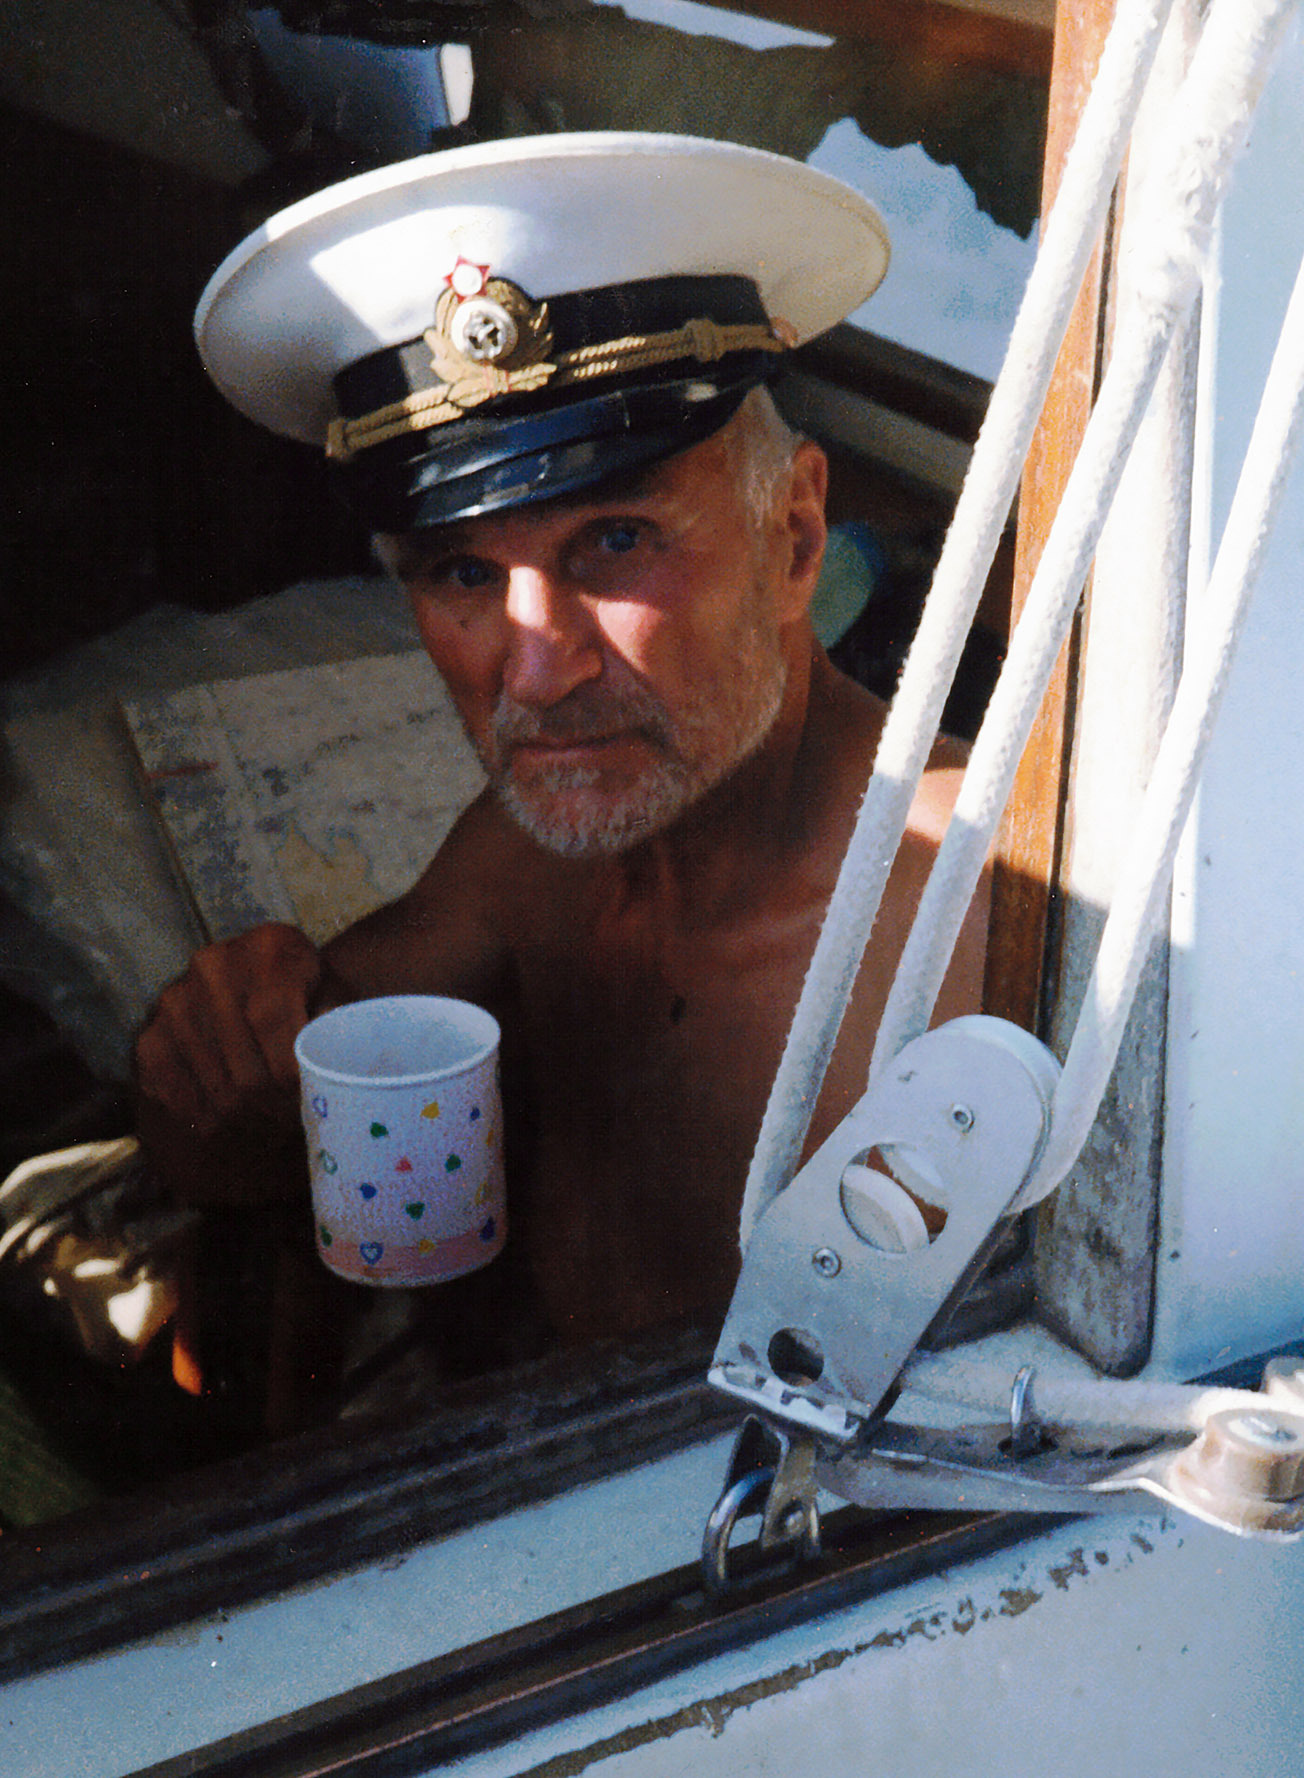
\includegraphics[width=3.2in,scale=1]{img/sailor_gpa_small_crop.jpg}}}
\AddToShipoutPicture*{\put(15,412){\textcolor{DarkBlue}{\textit{Bymba the Sailor Man.}}}}

\AddToShipoutPicture*{\put(15,22.5){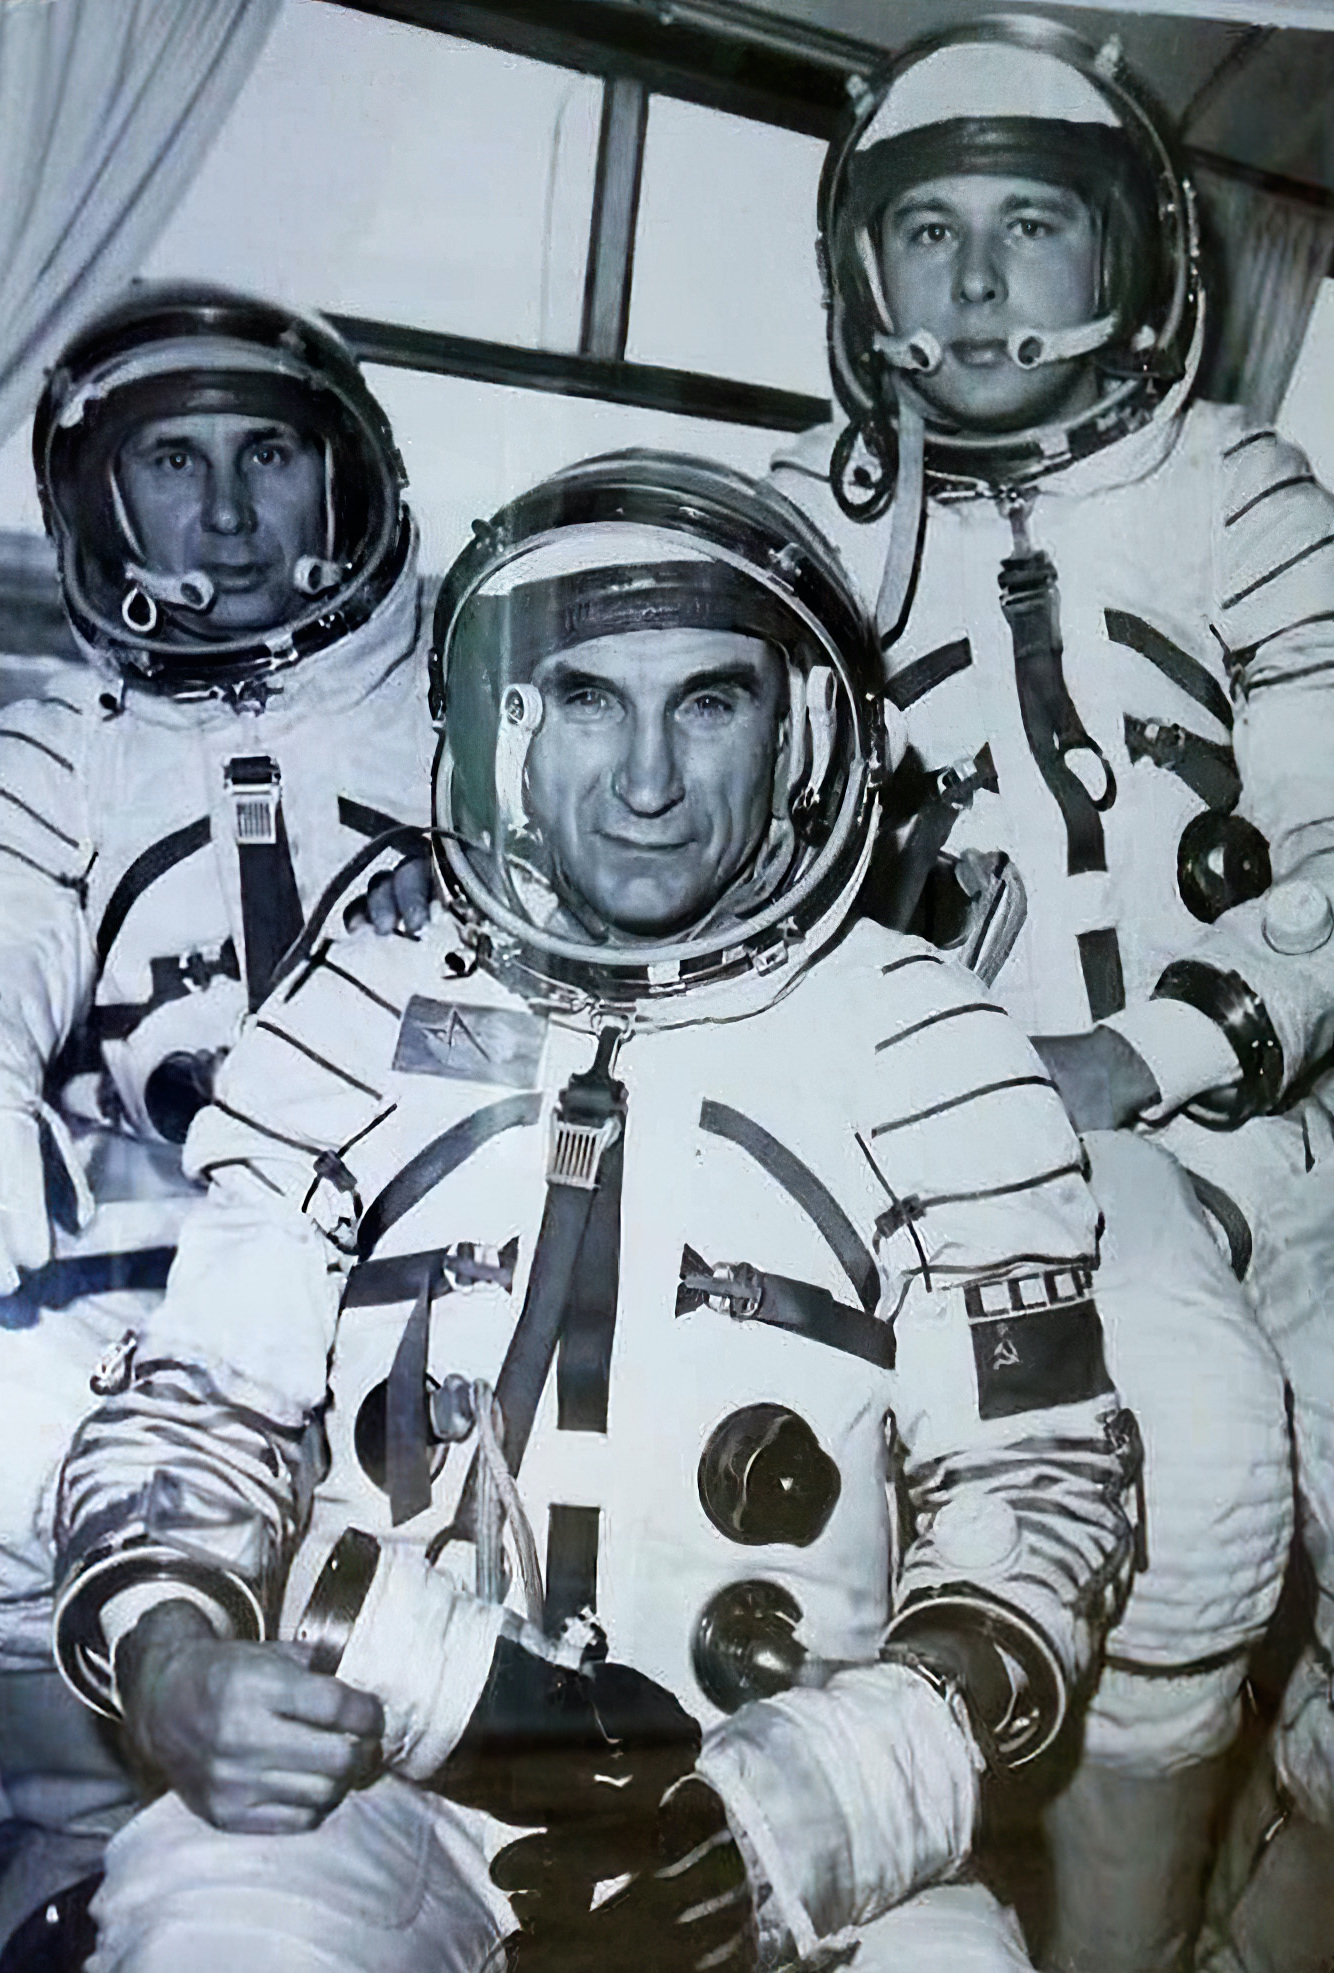
\includegraphics[width=3.2in,scale=1]{img/bymba-v-skafandre-2-big.jpg}}}
\AddToShipoutPicture*{\put(15,370){ \textcolor{DarkBlue}{\textit{With the crew.}}}}

\AddToShipoutPicture*{\put(215,51.5){
\includegraphics[width=1.5in, height=8.8in,scale=1]{img/white.png}}}

\lettrine{Y}{} esterday morning at 5:30 AM my grandfather died. 
\\
We were close. Closer, I dare say, than most. My own having father passed when I was very young, Grandpa Kostia – or Bymba, as I first called him – quickly assumed the mantle of my raising. Of any single individual he plausibly had the greatest influence on my childhood development, both through his direct mentorship as well as more indirectly, an example for my own growth. I spent many thousands of hours in his company, on walks through the woods and deserts, tending the plants of our dacha, swimming in backcountry lakes and overchlorinated pools, looking at the stars and the moon’s craters and the conjunctions of planets. He took me on cross-country trips, on overnight train rides to distant cities, through squares and museums and space centers. Calling upon half-borrowed connections, he clad me in scuba gear and chucked me into the pool at the Gagarin Training Center while hopeful cosmonauts practiced EVAs. In the motherland he was at home, and exerted himself in the service of my betterment.
\\\\
In even more distant lands and distant straits, he’d wait patiently for untold hours as I read through lengthy book series while lounging on grocery store patio furniture, or else stand around browsing utterly uninteresting electronic labels as I played video game demos. He designed many structured activities for us to do, scavenging old wood and canvas from dumpsters to build sailboats and hang gliders, hiding the disarticulated “skeletons” of “baby dinosaurs” for me to find in the miles of land surrounding our home, undertaking ill-conceived supplemental feeding campaigns for local insect populations, and hurling objects of myriad shapes and sizes back and forth across long distances separated by open fields. His more explicit lessons were sometimes strange – when beset by attackers, the eyes, groin, and throat make the most vulnerable targets – but those were easily filed away in the uncomfortable hope of never having to be used. We played thousands of seated games, of chess and checkers, dominoes and go, and favorite of all – the fool, which I left him more often than not. All together, we threw perhaps a million darts and basketballs, pinkies and rocks. Neither of us was ever very good. 
\\\\
Until his mid-seventies I thought him in excellent health. One summer in Phoenix, AZ, I took him on a quick midday hike up a local mountain along an exceptionally steep and scrambly “trail” that, in retrospect, I may have invented of whole cloth. As we neared the top, I noticed him swaying slightly, and breathing not through his nose but through his open mouth! Where was the man who’d so effortlessly fling me through the air, who’d happily brave with me and my unfortunate, un-consenting baby brother (in rickety push stroller) the 50C heat as we fetched groceries, who’d toss boomerangs in unshaded fields, sustain first degree burns on scorching playground equipment, and search for quarters on the streets that we might buy cold, refreshing carbonated beverages from discount vending machines? The vicissitudes of age were uncompromising indeed.

\tikzoverlay[text width=7in] at (-1.8in,8.25in) {
  \LARGE{The Seven Lives of \textcolor{DarkRed}{Konstantin Vetr}}
};

Before easy telecommunications arrived, we were unable to interact much during times apart. But Bymba nevertheless made do, sending me many dozens of letters inquiring after and commenting on my own affairs, describing his comings and goings throughout Russia, and always including some sort of hand-drawn puzzle for me to solve, often requiring the application of both verbal and mathematical reasoning.
\\\\
But by my mid-teens cell phones had grown commonplace, so we were able to maintain a regular telephone habit after my departure from hearth and home. Almost every morning on my walk into school or work, I’d give him and grandma a call. He’d rarely pick up, but she usually would, if on the second or third attempt, and hand the phone over after we finished speaking ourselves. For want of deeper conversation, I eventually happened upon a most devious strategy: a relentless bullying campaign replete with provocation, shame, and harassment. Over the last decade I imported and forced him to read many dozens of books – mostly translations of Western pop-sci, history, philosophy, and fiction I'd grown up reading – and then pirated \& photo-copied, enlarged, and printed out dozens more after claims of poor vision began surfacing. During those morning chats and after not inconsiderable nagging, I’d extract from him a book report on the initially 10-20 but eventually 1-2 pages he'd read the day before, and we’d discuss its finer points in detail. The fiction was rarely to his liking (Sagan’s \textit{Contact} being the rare exception, though Robinson's \textit{Mars} trilogy and Weir’s \textit{Martian} were also tolerable), but he certainly enjoyed the non-fiction, breathlessly recounting “new” insights from cosmology, genetics, astrophysics, paleontology, and other disciplines. At times, we’d deviate from this pattern, with me substituting reading homework with 3-D puzzle homework, or even cutting him a break by assigning whatever Russian-dubbed TV shows I'd recently taken interest in, but by and large we were able to get through several dozen works from almost just as many authors and topics.
\\

\AddToShipoutPicture*{\put(370,425){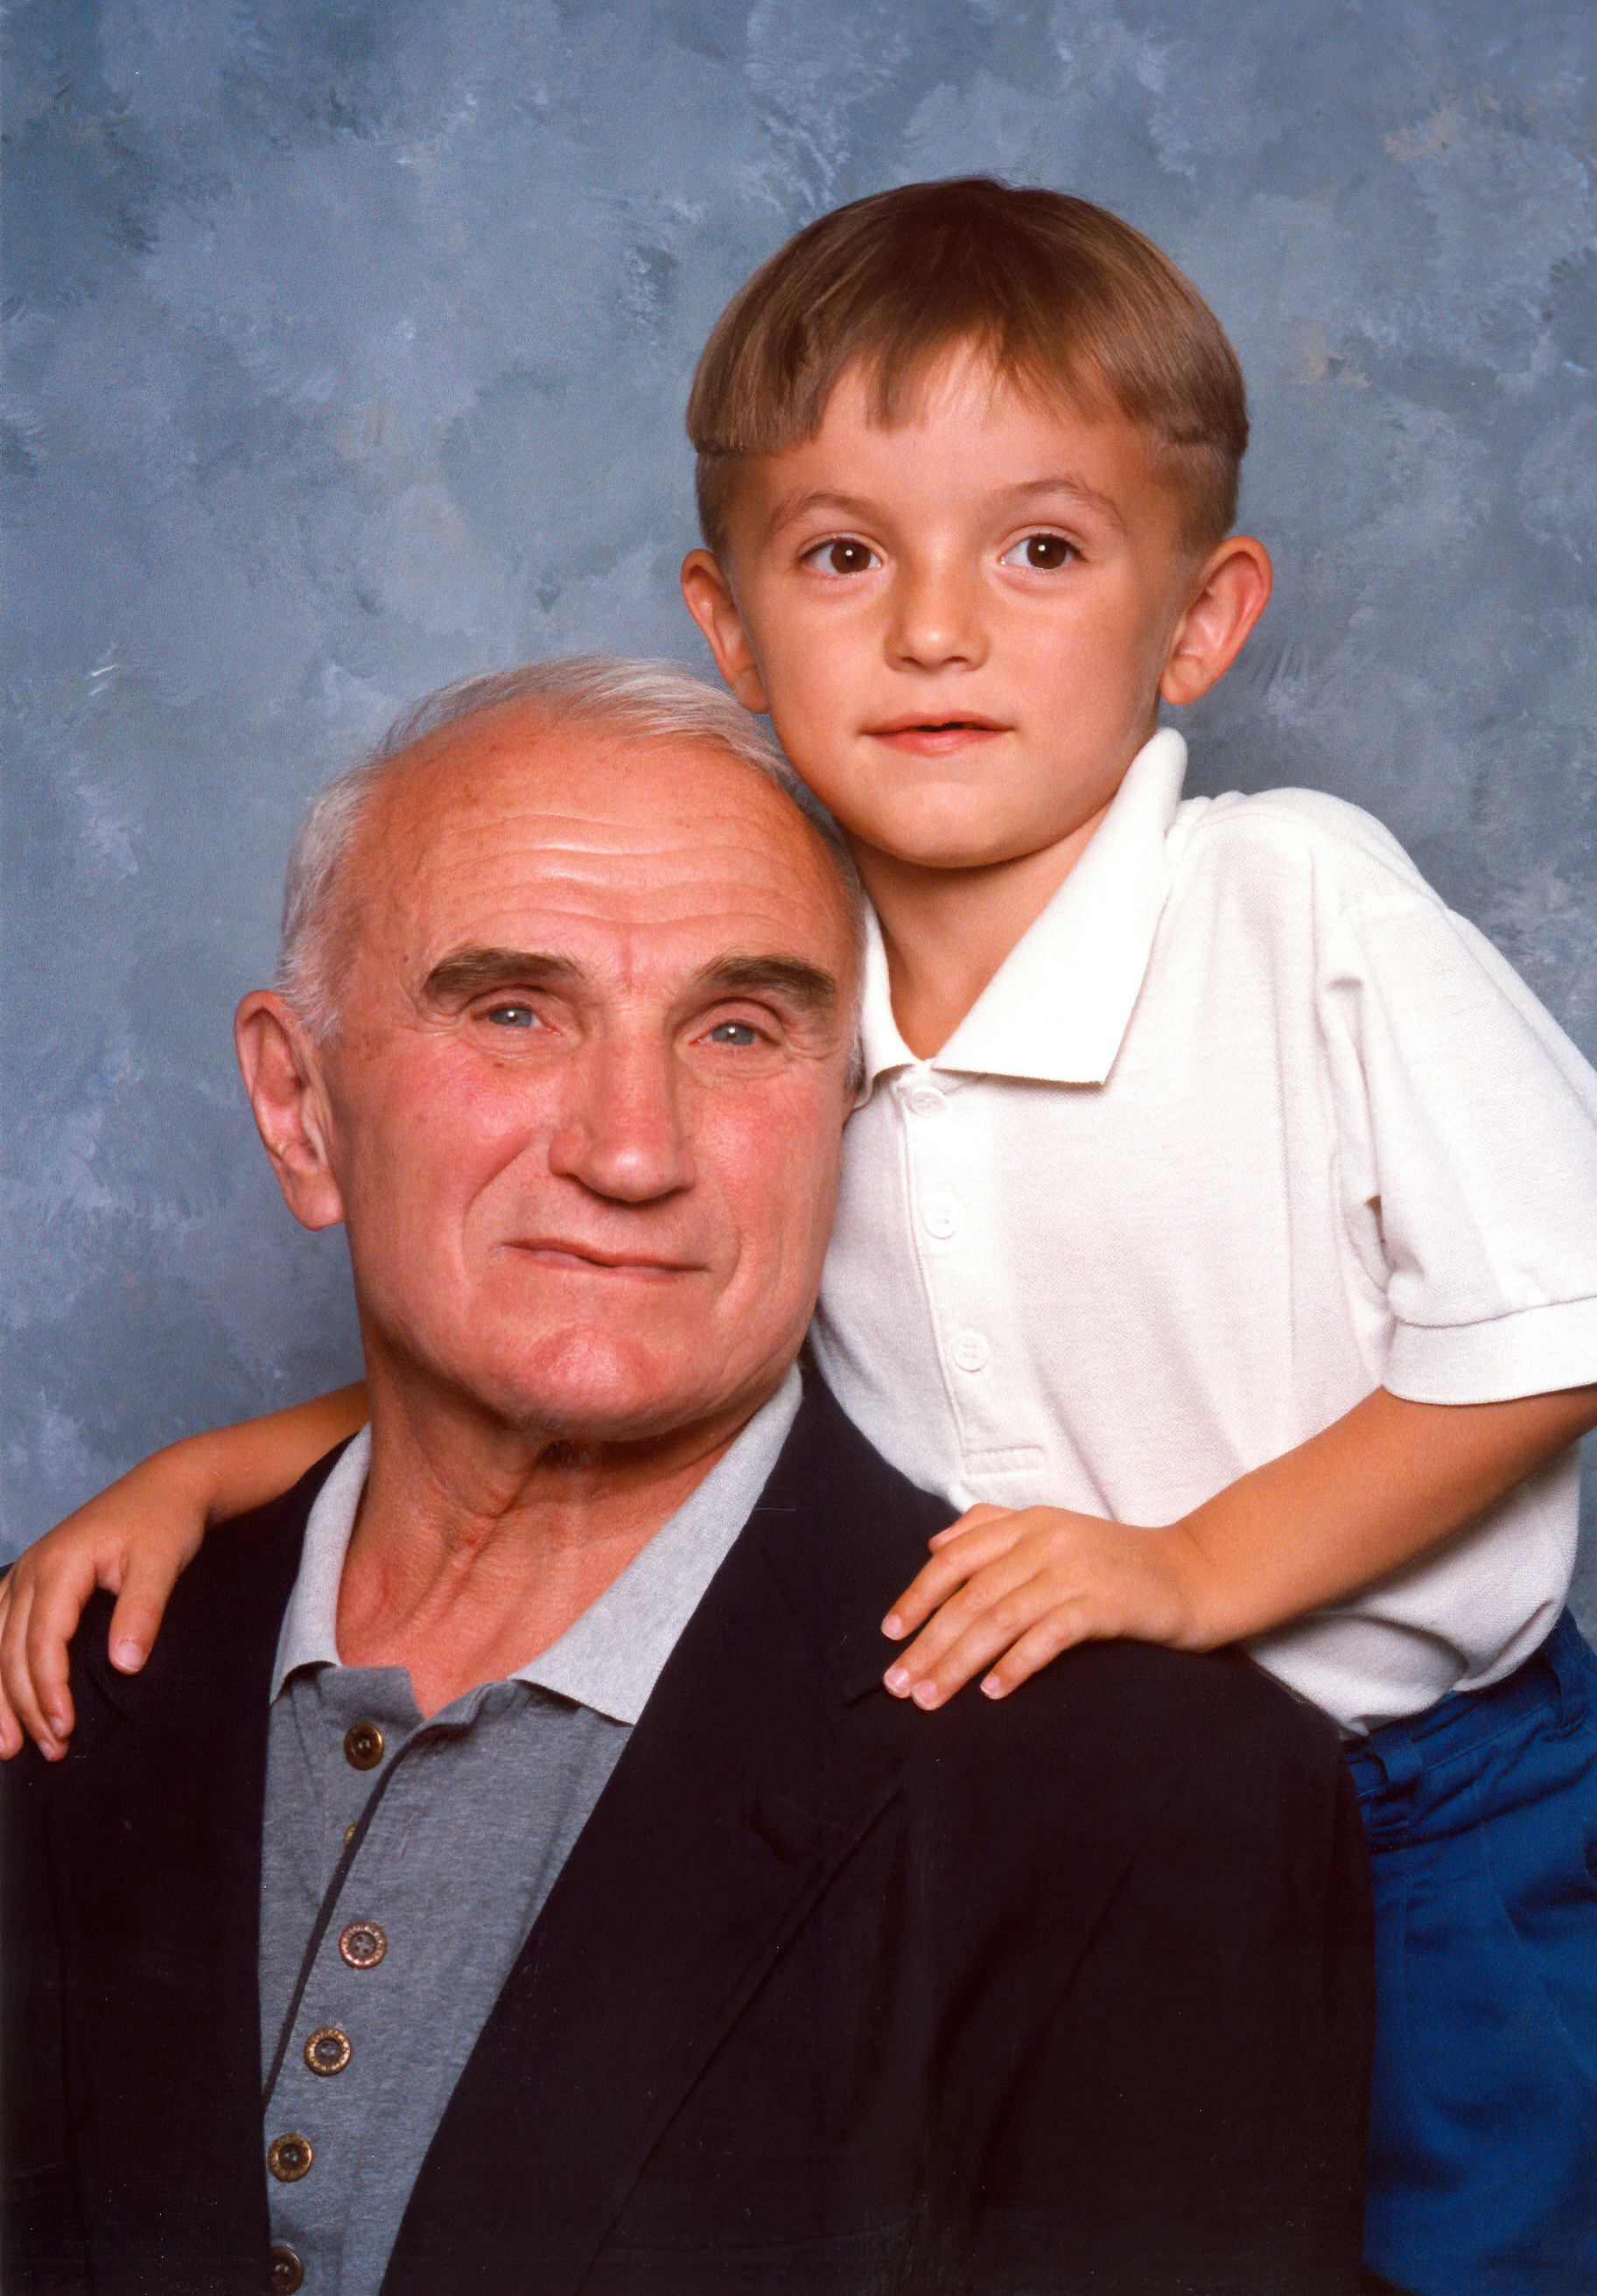
\includegraphics[width=3.175in,scale=1]{img/Me_Grandpa_2-sharpen.jpg}}}
\AddToShipoutPicture*{\put(398.4,77.5){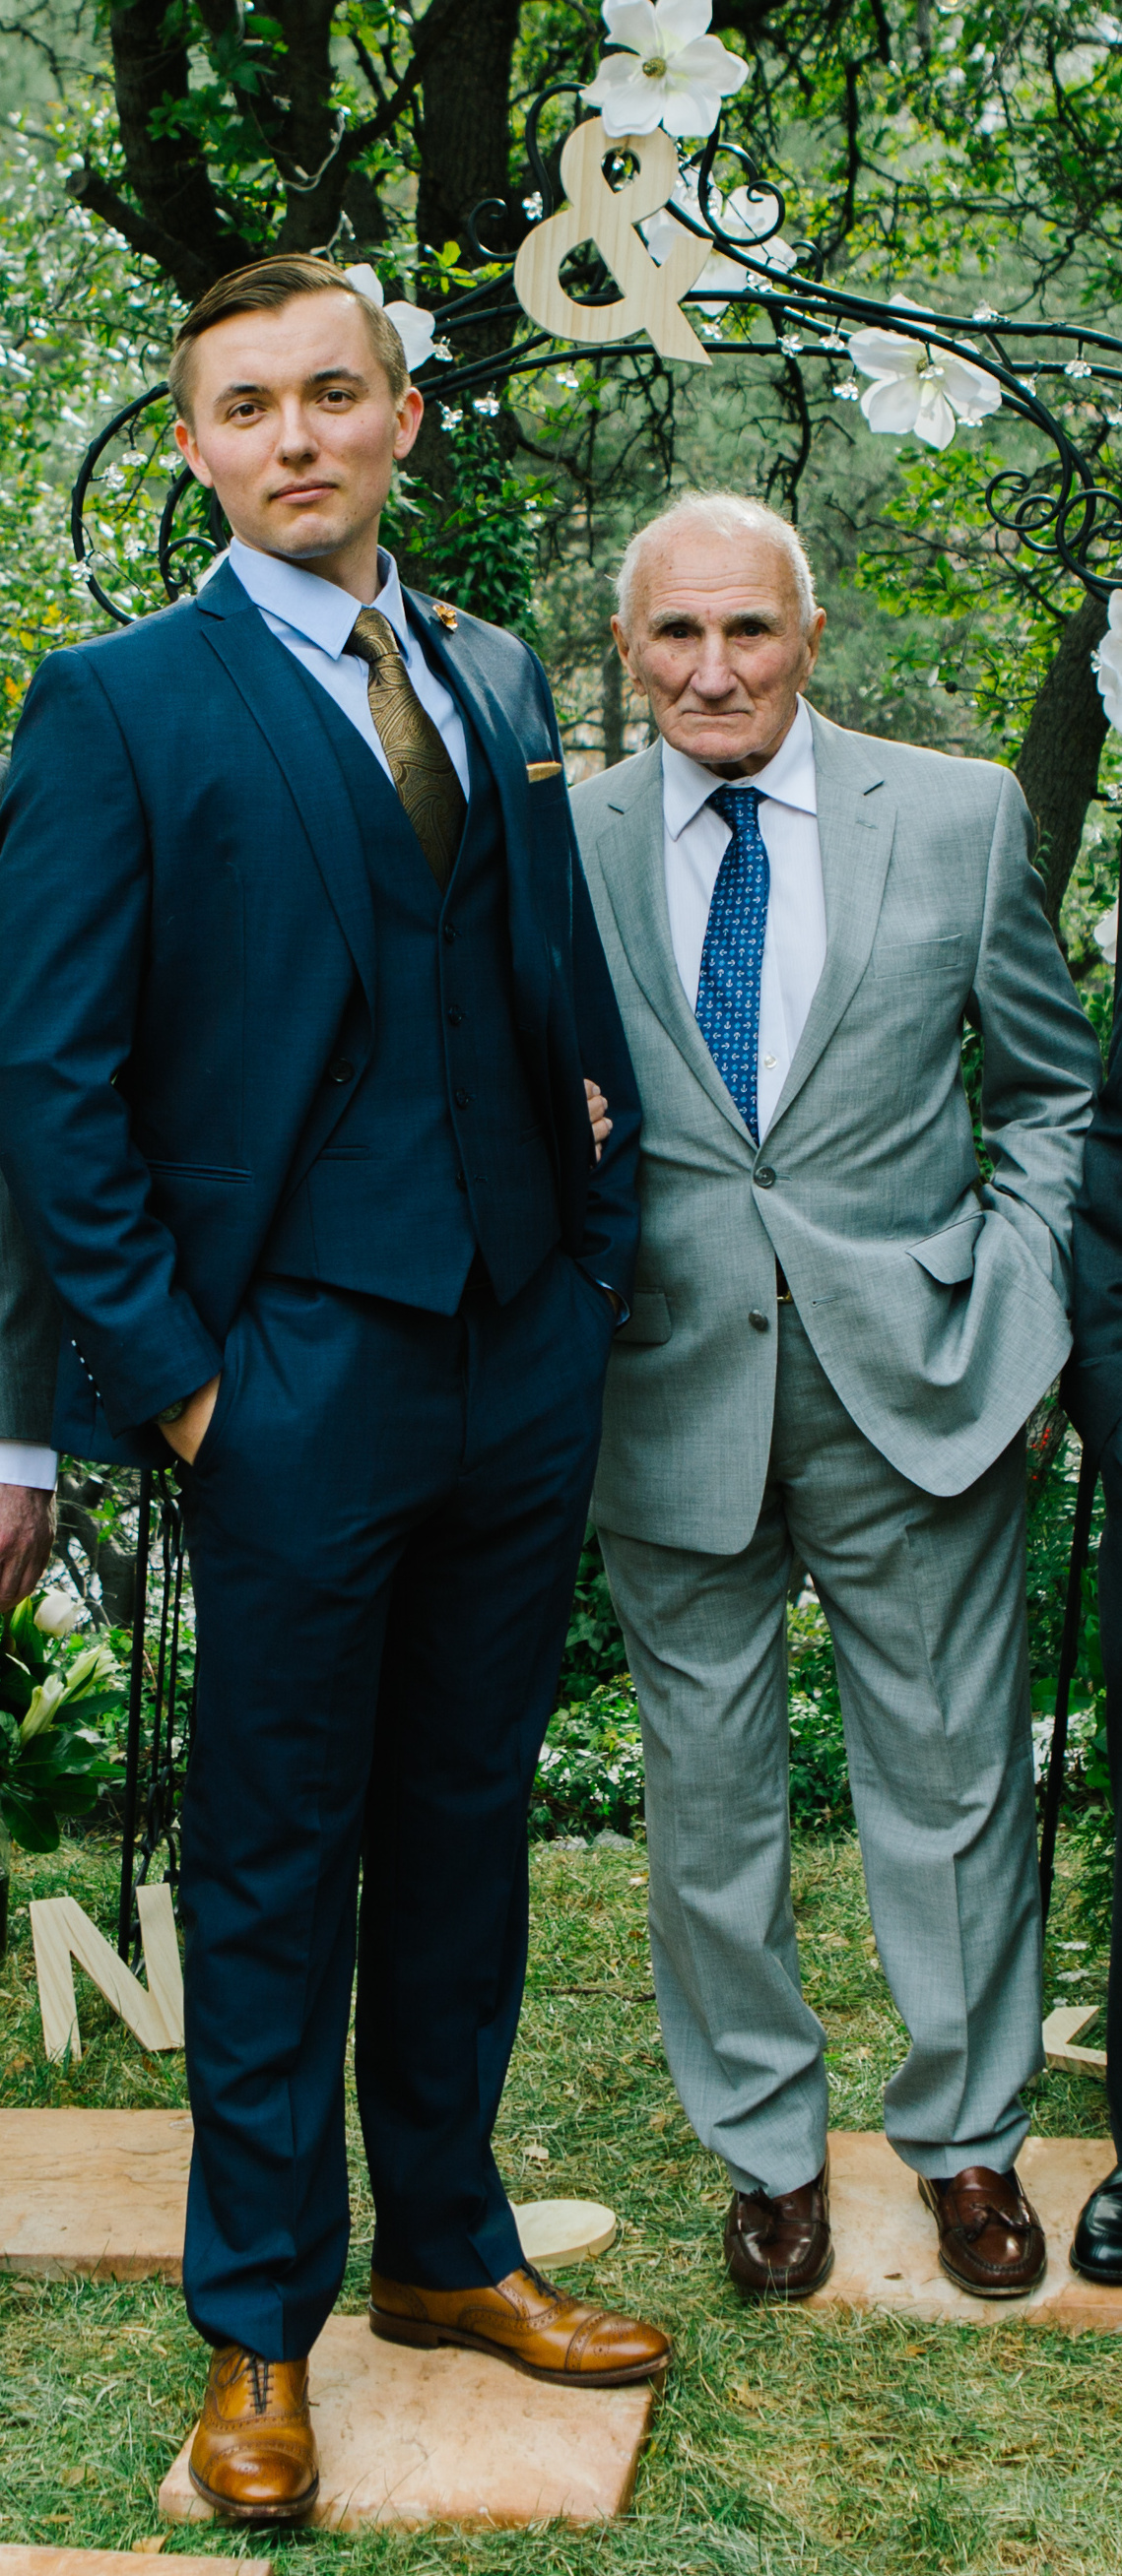
\includegraphics[width=2.05in,scale=1]{img/serious_wedding.jpg}}}
\AddToShipoutPicture*{\put(398.4,67.5){\textcolor{DarkBlue}{\textit{Two trouble-makers.}}}}
\AddToShipoutPicture*{\put(290,51.5){
\includegraphics[width=1.5in, height=8.8in,scale=1]{img/white.png}}}
I was unfortunately unable to reach him in his final moments – the phone call arrived just as I was packing to leave for a morning flight out, and his death was sudden enough that my request for updates on his condition, that I might drive or fly out sooner, went unfulfilled. But outside some sort of peak-end bias, I’m not sure it’s quite right to privilege certain person-moments over others. If anything, later moments seem of lower priority for their inability to psychologically influence whatever succeeds them. Bymba was a proud man, and likely would not have wanted to be seen in the condition that characterized his passing. That said… I’d have wanted nothing more than to hold his hand, reading papers, writing code, and taking meetings from his bedside. Instead, our last interactions were some weeks prior, at such time as he could still shuffle about the house and yard. He gifted me a watch that he’d received from his friend Georgy Beregovoy many decades ago, a Raketa World Time, and we went through all the cities listed on the bezel and recounted to each other our respective experiences in each. We played several games of chess, cards, and dominos, almost evenly matched. We ate together and enjoyed one another’s company. I’m sorry I couldn’t be with you in the end, Bymba, but I hope our last moments together were enough.
\\\\
(if anything, we’re now even, you having missed my own birth by months while off on some sailing adventure. For just as with your exit, I came into this world prematurely)
\\\\
Surprisingly, Bymba also existed prior to my birth. Over those sixty-some years, his accomplishments were many, enough to fill several lifetimes. He was a sailor, sportsman, \& storyteller, a cosmonaut \& steadfast companion, an engineer \& trickster. He designed rocket boosters and atmospheric reentry capsules, spent thousands of hours training for missions alongside or under his friends Kamanin, Gagarin, and Korolev, and sailed across many seas and oceans, both as part of a larger crew and alone. He was a \href{https://en.wikipedia.org/wiki/Unified_Sports_Classification_System_of_the_USSR_and_Russia#Athletes}{Master of Sport} in yachting and skydiving, setting many records across 2,000+ jumps. In boxing and cross-country skiing, he merely competed in the Second-Class, but could perform many impressive feats of athleticism, such as 45 consecutive non-kipping pull-ups. Even unto his eventual confinement in bed and subsequent death, he continued to do his daily exercises, though they eventually dwindled from the hoisting of makeshift atlas stones to the pressing of lightweight dumbbells. Always a bit of a peacock, he enjoyed having his feathers preened by my advertisement via \href{https://www.reddit.com/r/IAmA/comments/etu2s/i_was_born_in_shchigry_ru_in_1932_i_worked_as_a/}{interviews} and \href{https://www.reddit.com/r/OldSchoolCool/comments/8473rx/what_56_years_of_marriage_does_to_a_couple/}{photos} on websites such as Reddit. And just as with every woman aged 18-80 to cross his path, he often flirted with other vocations, spending years driving tanks and diesel-powered submarines, playing the piano and guitar, and illegally building various personal transportation vehicles ranging from hot air balloons to helicopters. Between these, Nazi occupation, and exposure to radiation not far from the Chernobyl exclusion zone, it’s truly a wonder he did not die sooner, though I suppose serving as the protagonist of a Jules Verne novel did offer some protection.
\\\\
He loved to play pranks on his family and friends, and was a consummate cheat in games of chance and skill, though always in good fun, and always fessing up moments after his ill-earned victories. We’d get him back, in turn: a favorite childhood pastime of mine was watching him return to our apartment building laden heavily with groceries. After ringing him in, I’d rush to our floor’s lobby and quickly summon both elevators. In exchange for sending them to the top floor and resummoning them to our own a dozen times, I’d be rewarded by grandpa’s strained face emerging from the stairwell. Any lack of consideration for other building residents I rest entirely on his shoulders. And while not many still live with distinct memories of his deeds and misdeeds – the children of his colleagues and friends long dead from old age – several of them were compiled into an autobiographical memoir he wrote decades ago, featuring, as I’ve gathered, only the usual amounts of exaggeration and embellishment.
\\

\AddToShipoutPicture*{\hspace{0cm}\put(0,0){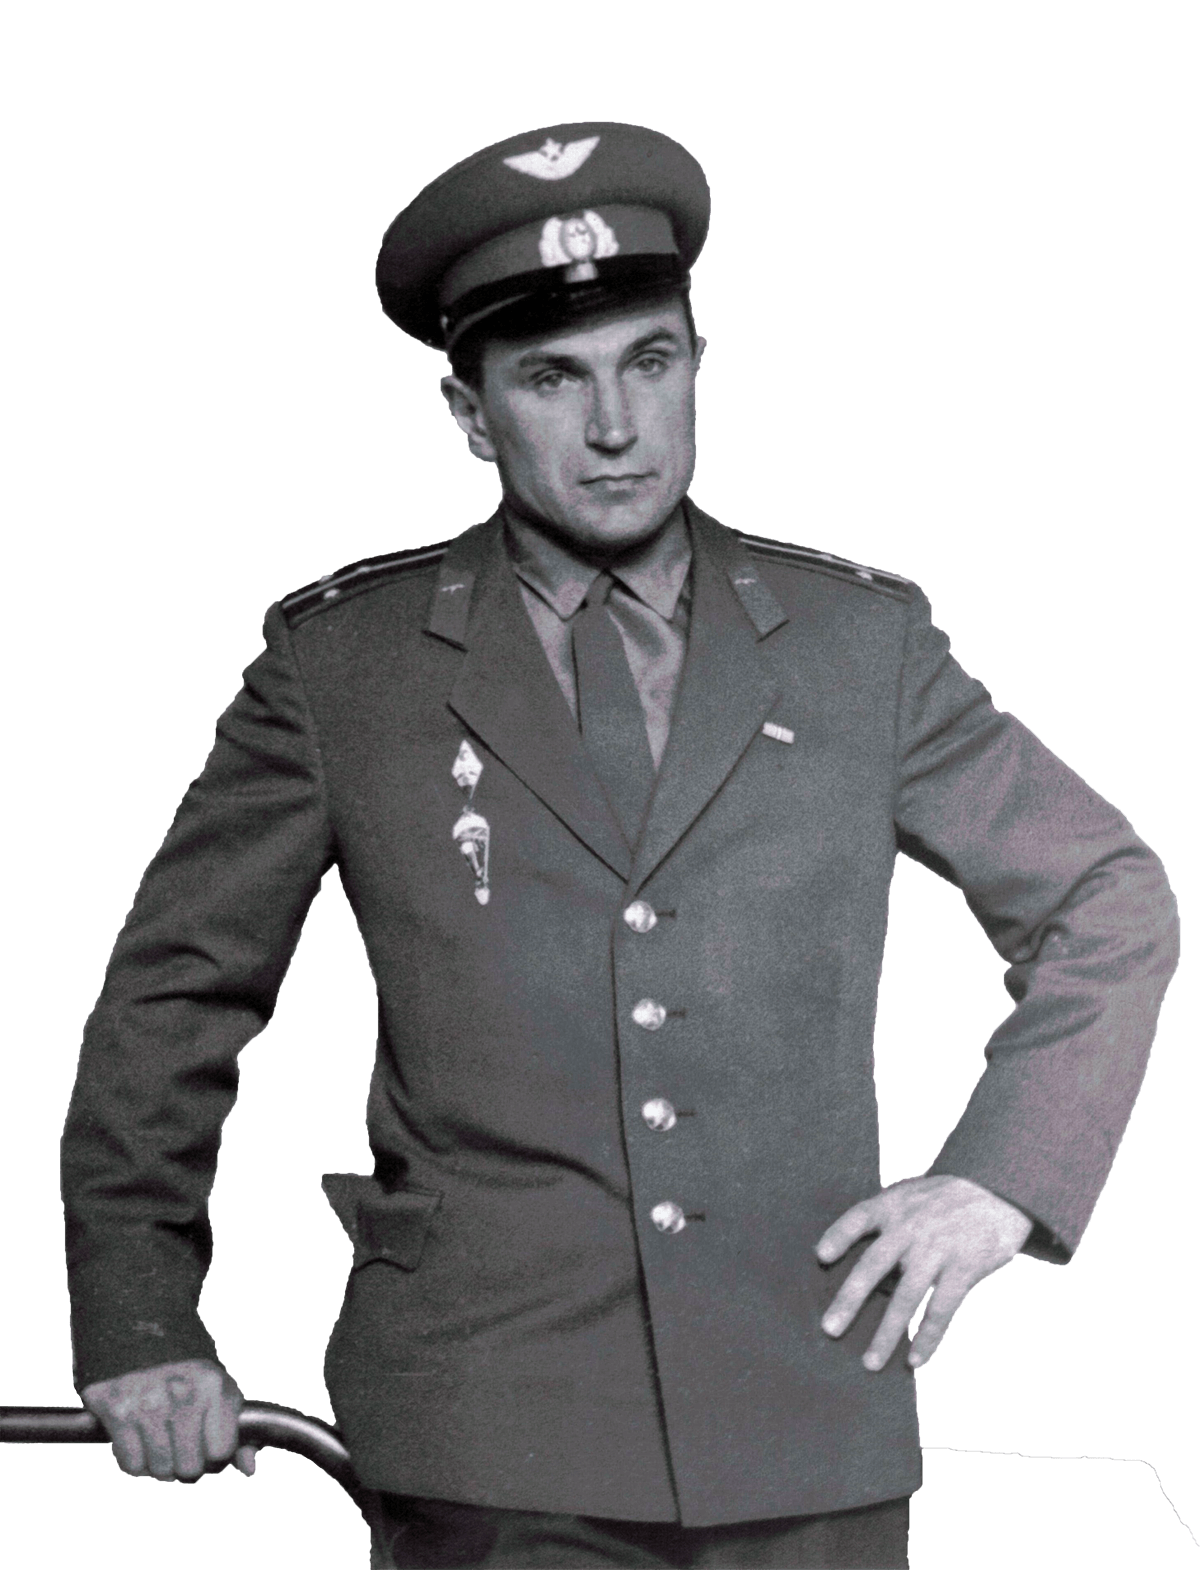
\includegraphics[width=3in,scale=1]{img/sassy_gpa_small.png}}}
\AddToShipoutPicture*{\hspace{0cm}\put(30,620){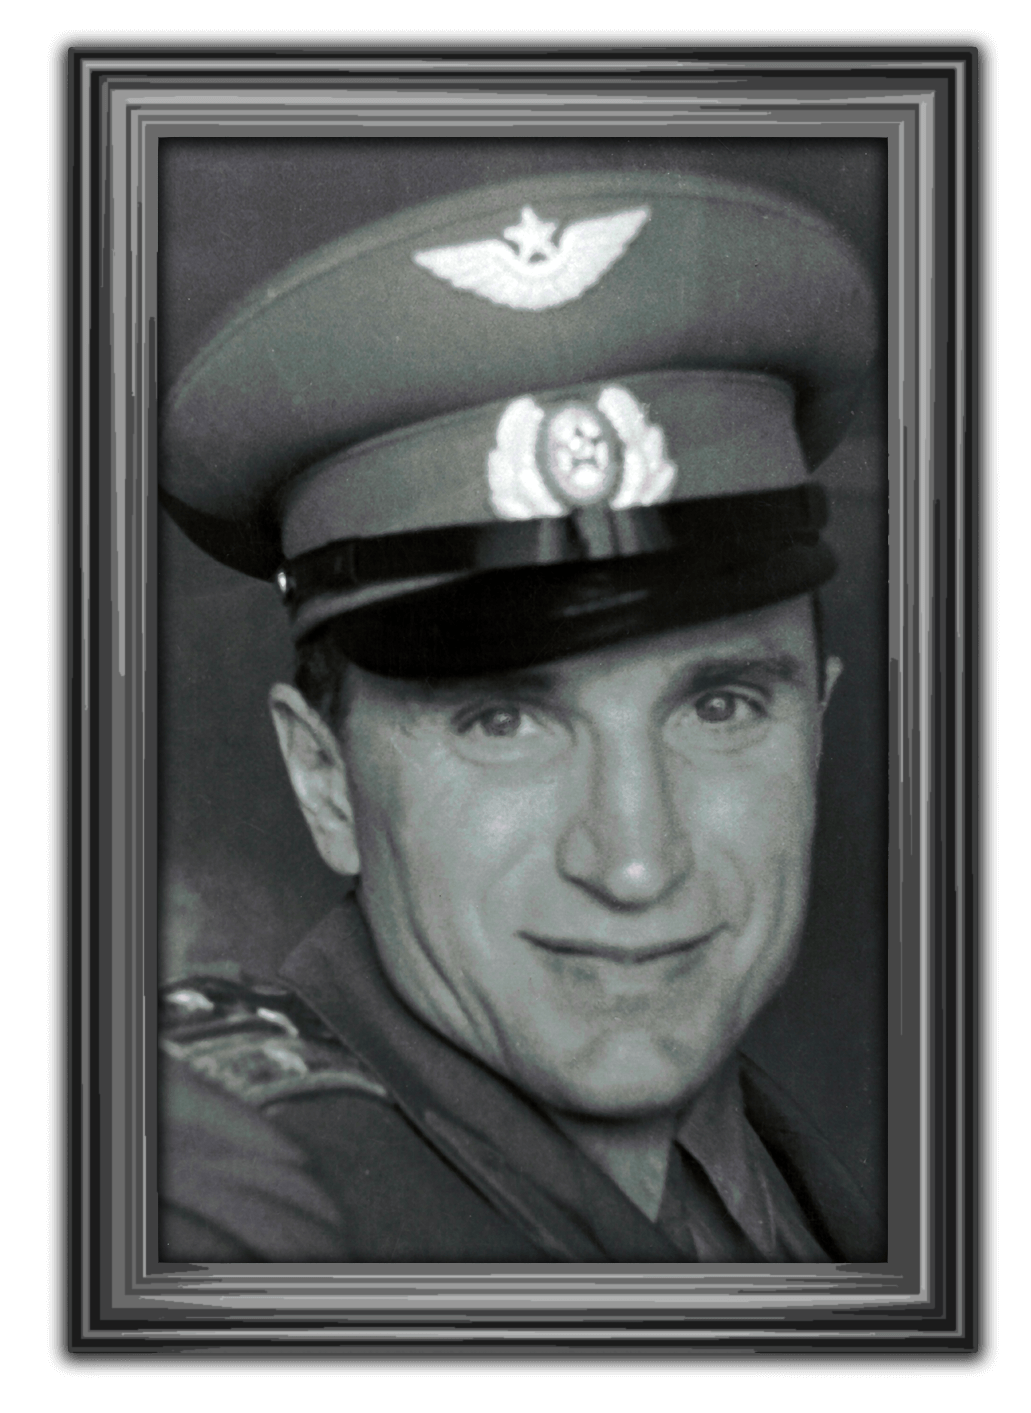
\includegraphics[width=1.5in,scale=1]{img/gpa_army_portrait_frame_small.png}}}
\AddToShipoutPicture*{\hspace{0cm}\put(55,435){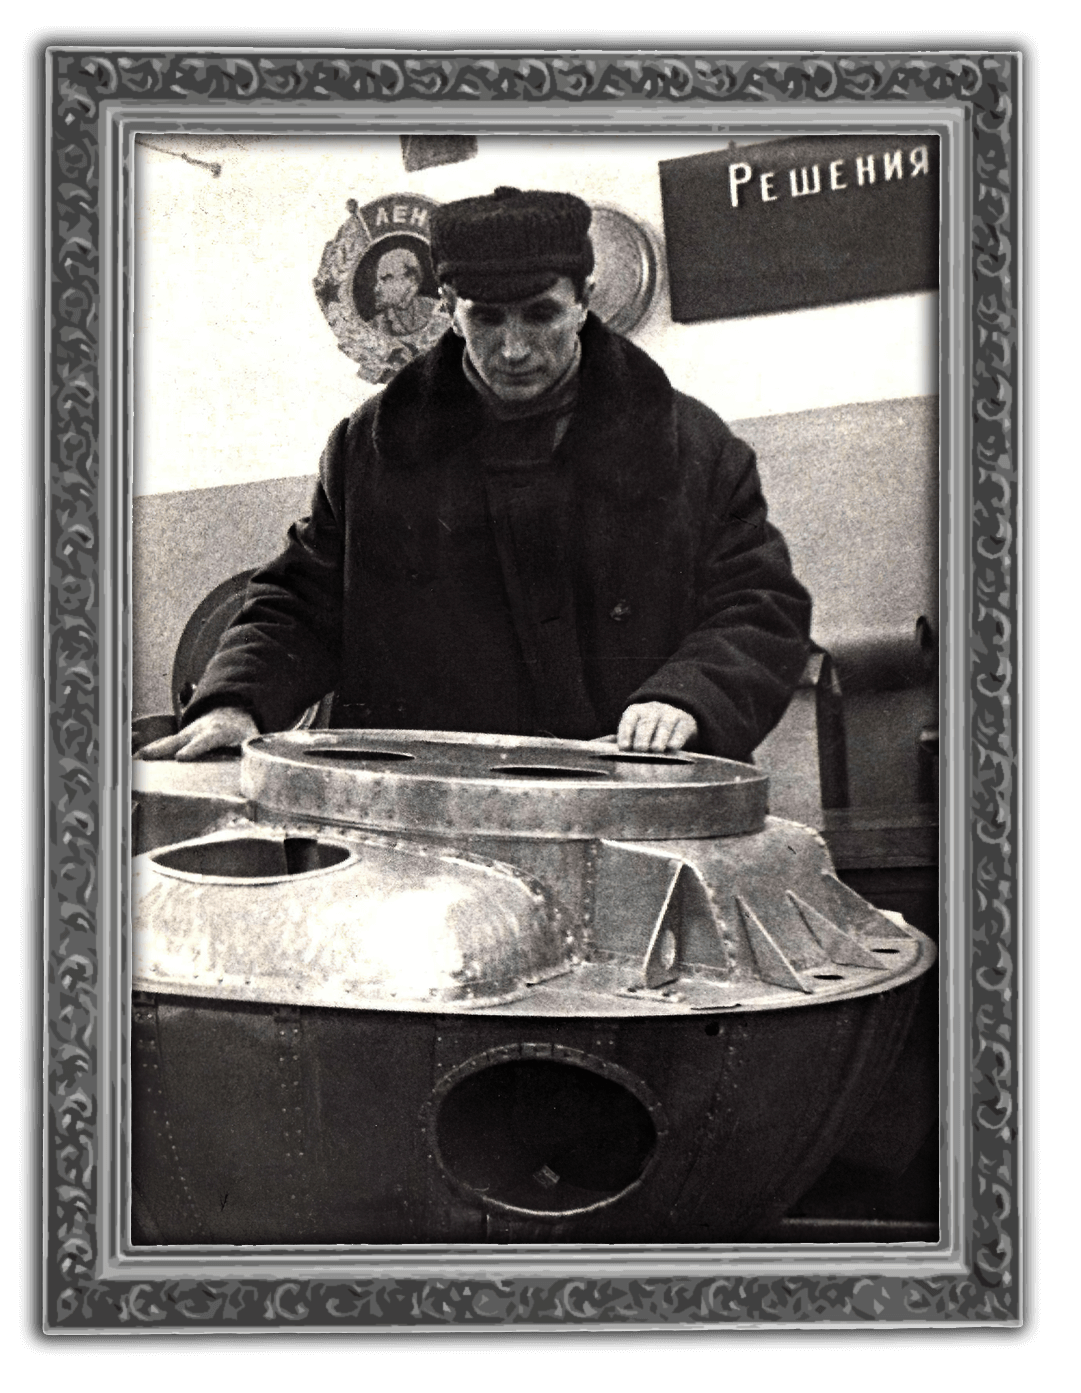
\includegraphics[width=2in,scale=1]{img/reentry_capsule_framed.png}}}
\AddToShipoutPicture*{\hspace{0cm}\put(40,280){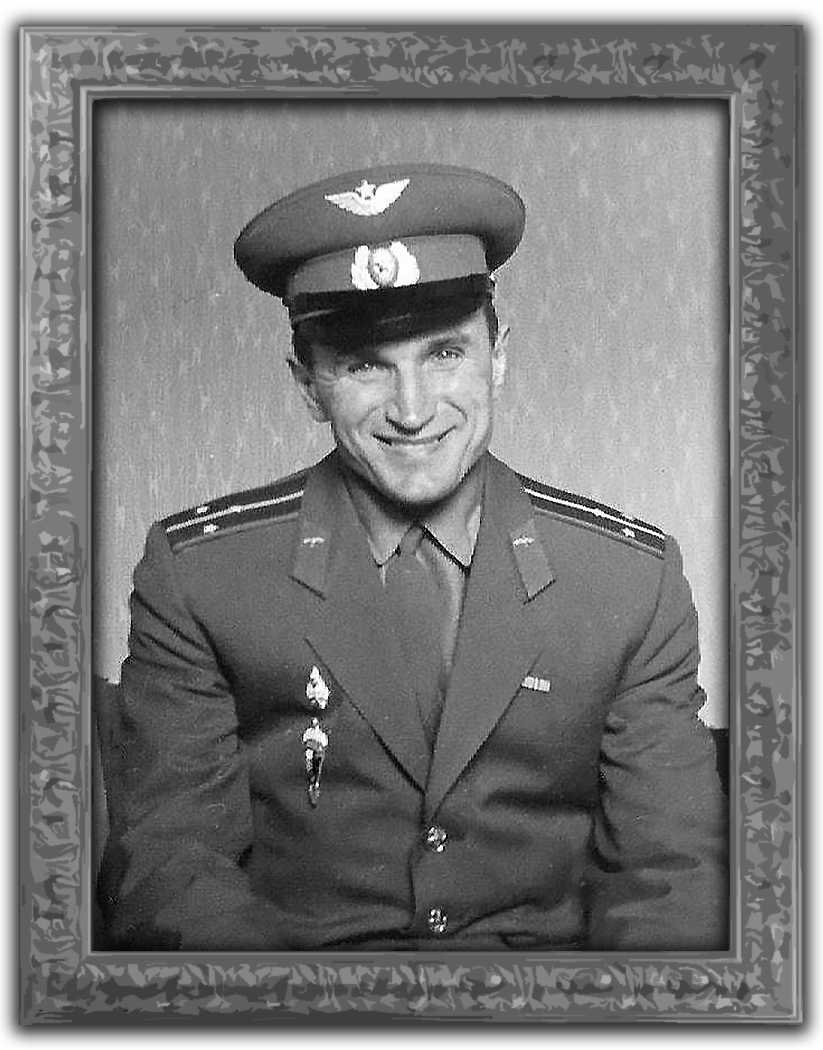
\includegraphics[width=1.65in,scale=1]{img/gpa_military_portrait_frame_shadow.png}}}
Of these and many other faults, Bymba, you also aspired quite strongly towards hypocrisy. Nothing but the strongest, blackest of coffees and teas for me, you’d proclaim, while happily mixing yourself a sugar-laden, coffee-flavored milkshake. Never has a drop of alcohol nor tobacco fume has entered my mouth! you’d announce while sipping from a glass of wine and smoking your yearly cigar. Soda is evil incarnate, quenching no thirst and rotting not only teeth but mind as well, you’d advise while purchasing our hundredth Big Gulp that year, to sit outside the gas station and play with me some bastardization of curling with scattered pebbles. Gambling, what a terrible sin; but do take these arcade tokens and booster packs, I’ve bought them for you. The spirit of adventure, how invigorating and thrilling! Yet you’d wait up until the wee hours for me to return from any overlong “day-hikes” or cross-country road trips, and how you fretted when I first began solo-backpacking in my mid-teens. I’m sorry for worrying you.
\\\\
At the end of every conversation, you would always promise the following: to always remember me, to always love me, and to always wait for me. It would appear that you have failed to keep this promise. I feel I cannot quite promise the same in return, for sheer physical impossibility, if nothing else. But while I don’t think there’s much left to wait for, remembrance and love of the man who raised me are two faculties as yet within my power. It’s not much, but it'll have to do.

\AddToShipoutPicture*{\hspace{0cm}\put(350,600){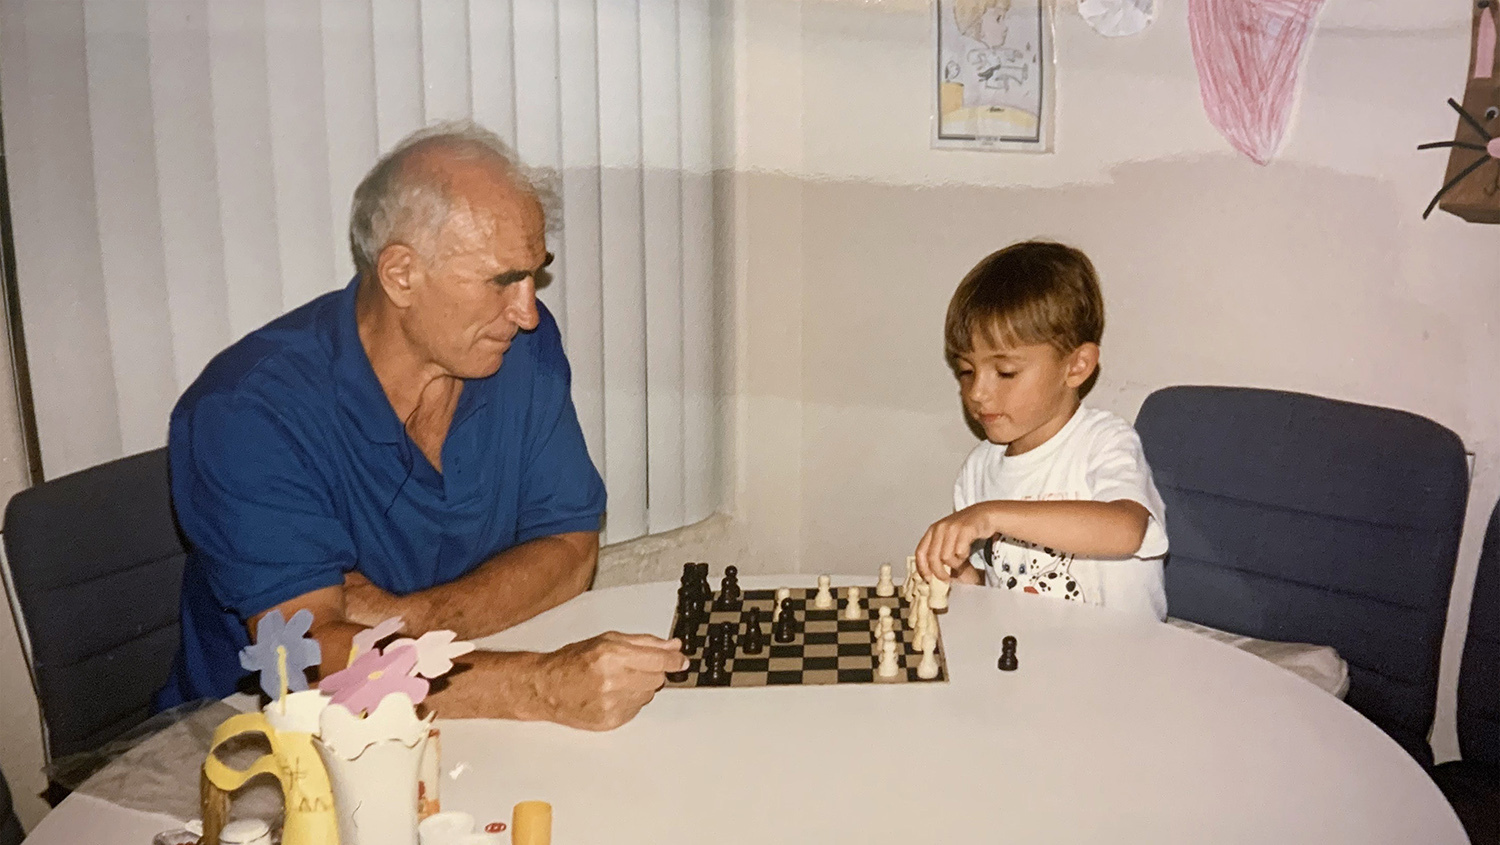
\includegraphics[width=3.5in,scale=1]{img/grandpa_me_chess_small.jpg}}}
\AddToShipoutPicture*{\hspace{0cm}\put(350,450){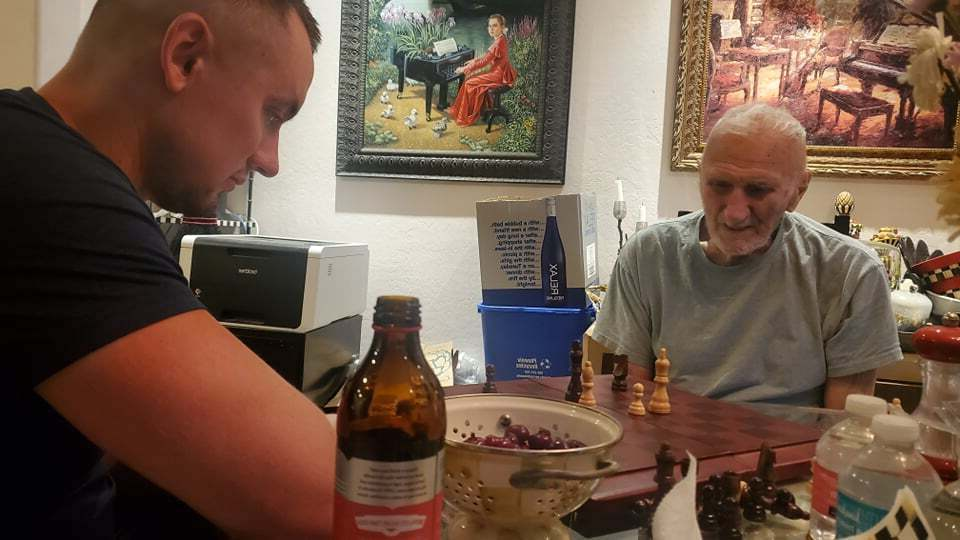
\includegraphics[width=3.5in,scale=1]{img/me_grandpa_chess.jpg}}}
\AddToShipoutPicture*{\put(290,490){
\includegraphics[width=1.5in, height=2.35in,scale=1]{img/white.png}}}
\AddToShipoutPicture*{\hspace{0cm}\put(350,438){\textcolor{DarkBlue}{\textit{First and last games.}}}}

\AddToShipoutPicture*{\hspace{0cm}\put(40,270){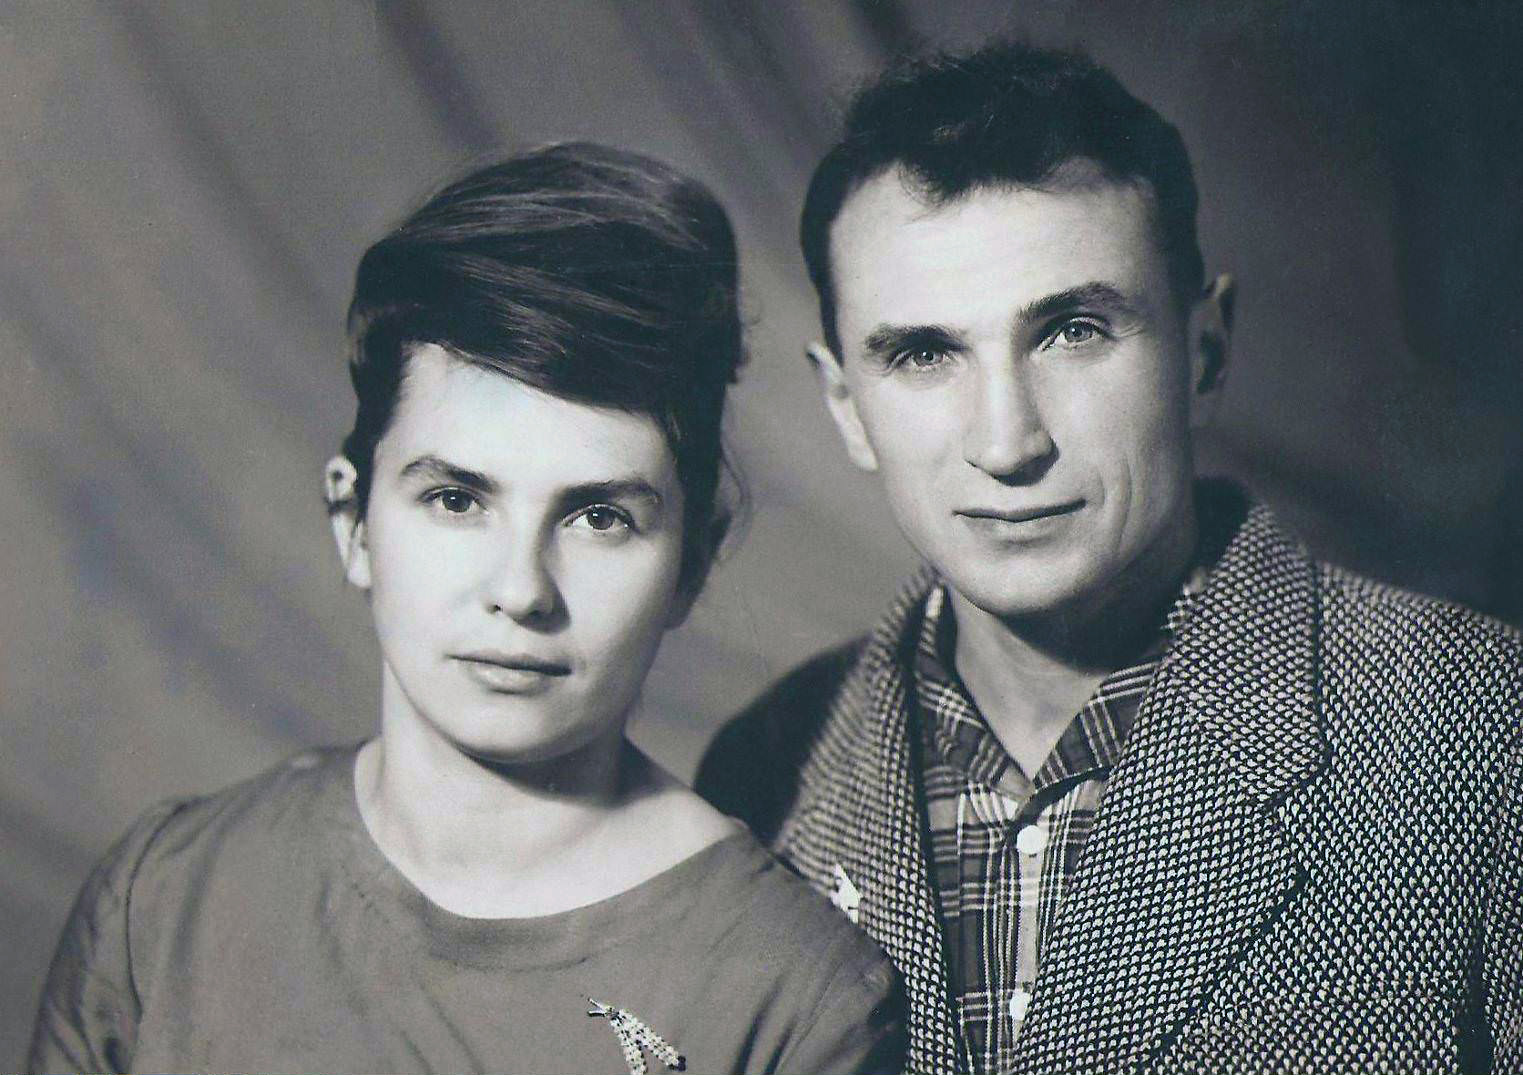
\includegraphics[width=4in,scale=1]{img/gma_gpa_old.jpg}}}
\AddToShipoutPicture*{\hspace{0cm}\put(40,30){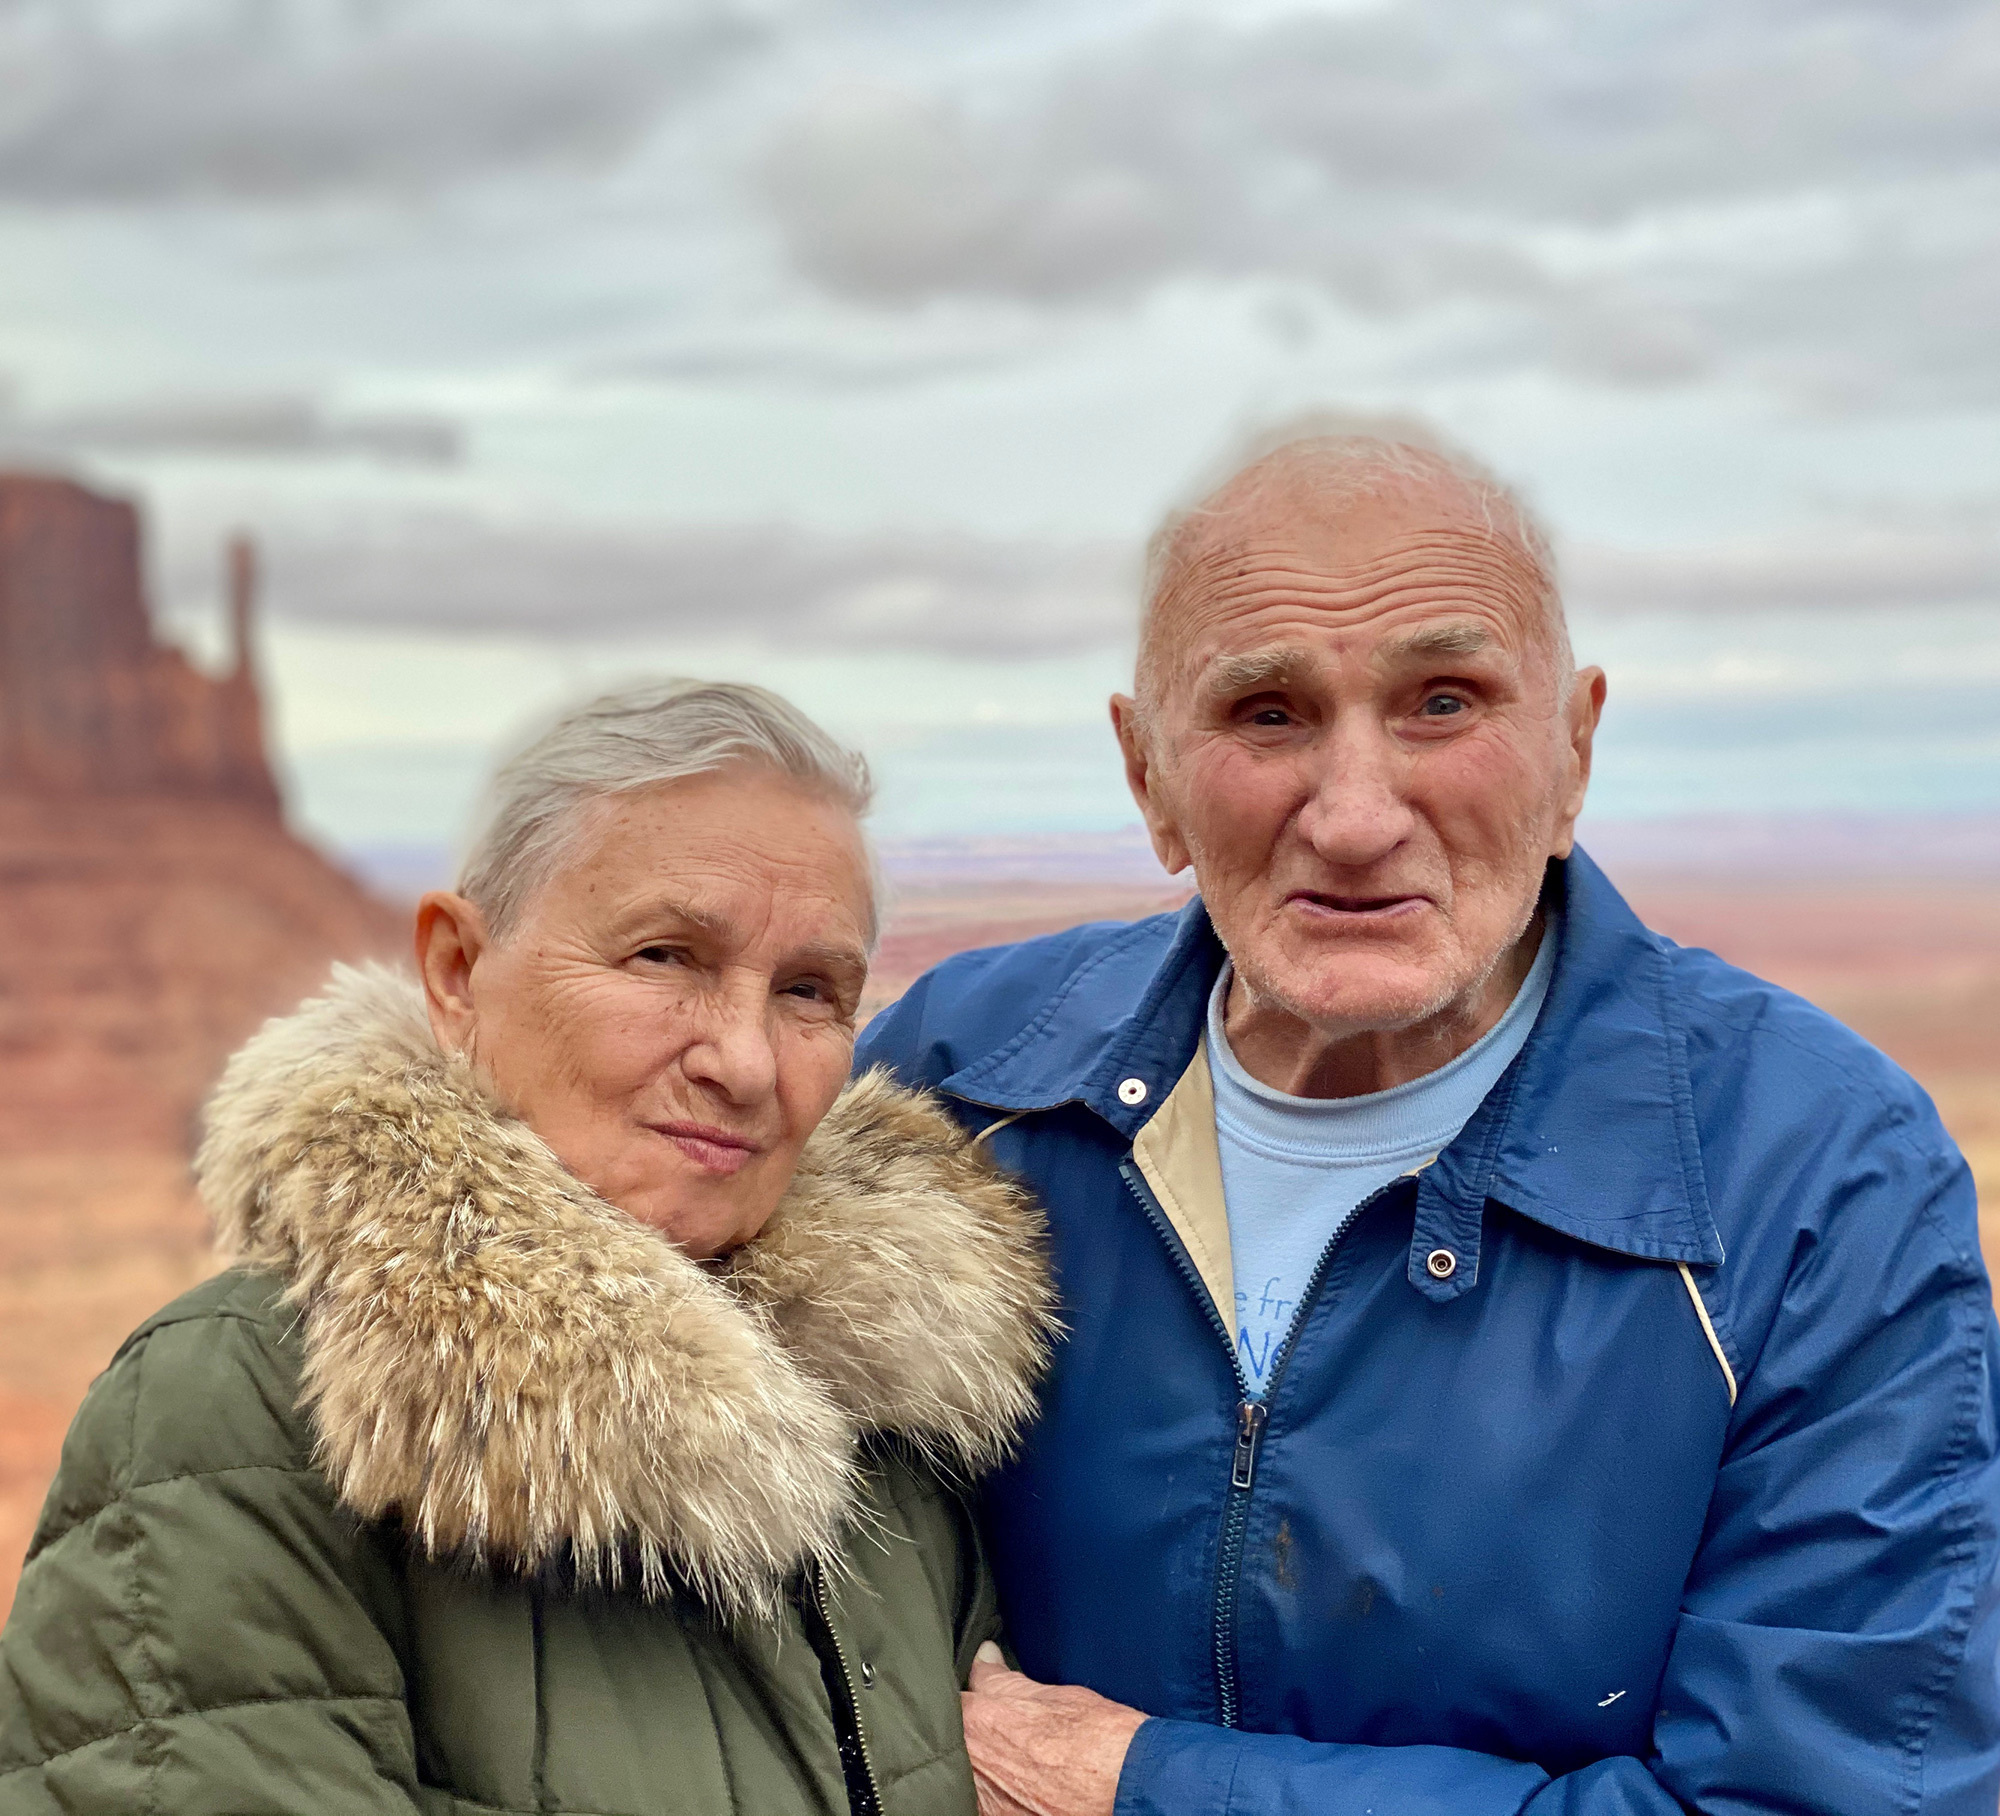
\includegraphics[width=3.5in,scale=1]{img/gparents_new.jpg}}}
\AddToShipoutPicture*{\hspace{0cm}\put(340,270){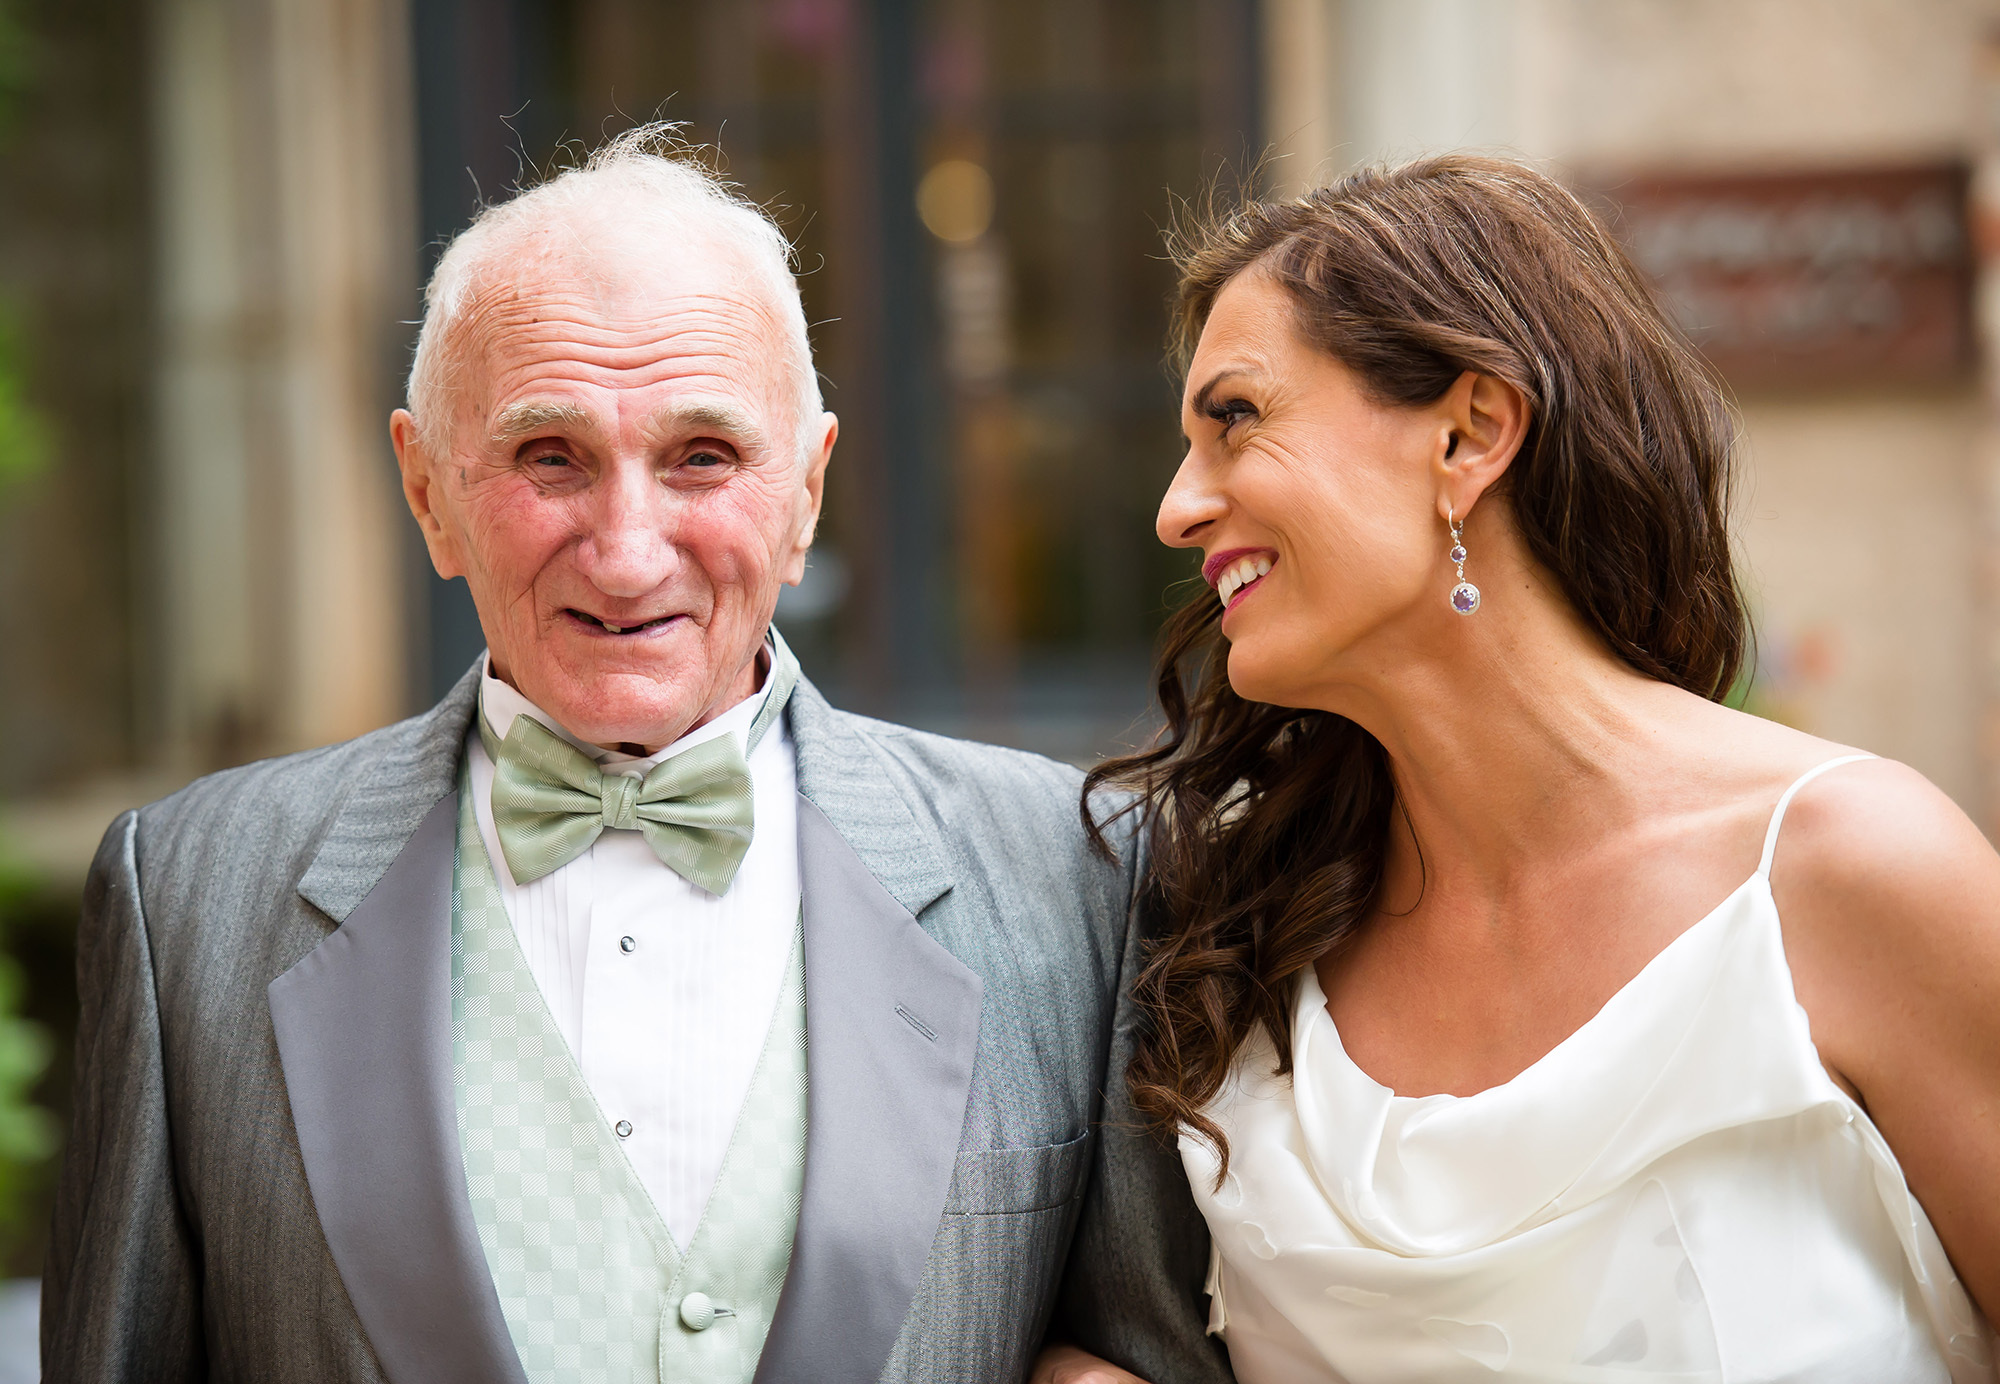
\includegraphics[width=3.15in,scale=1]{img/mom_gpa_small.jpg}}}
\AddToShipoutPicture*{\hspace{0cm}\put(305,73.5){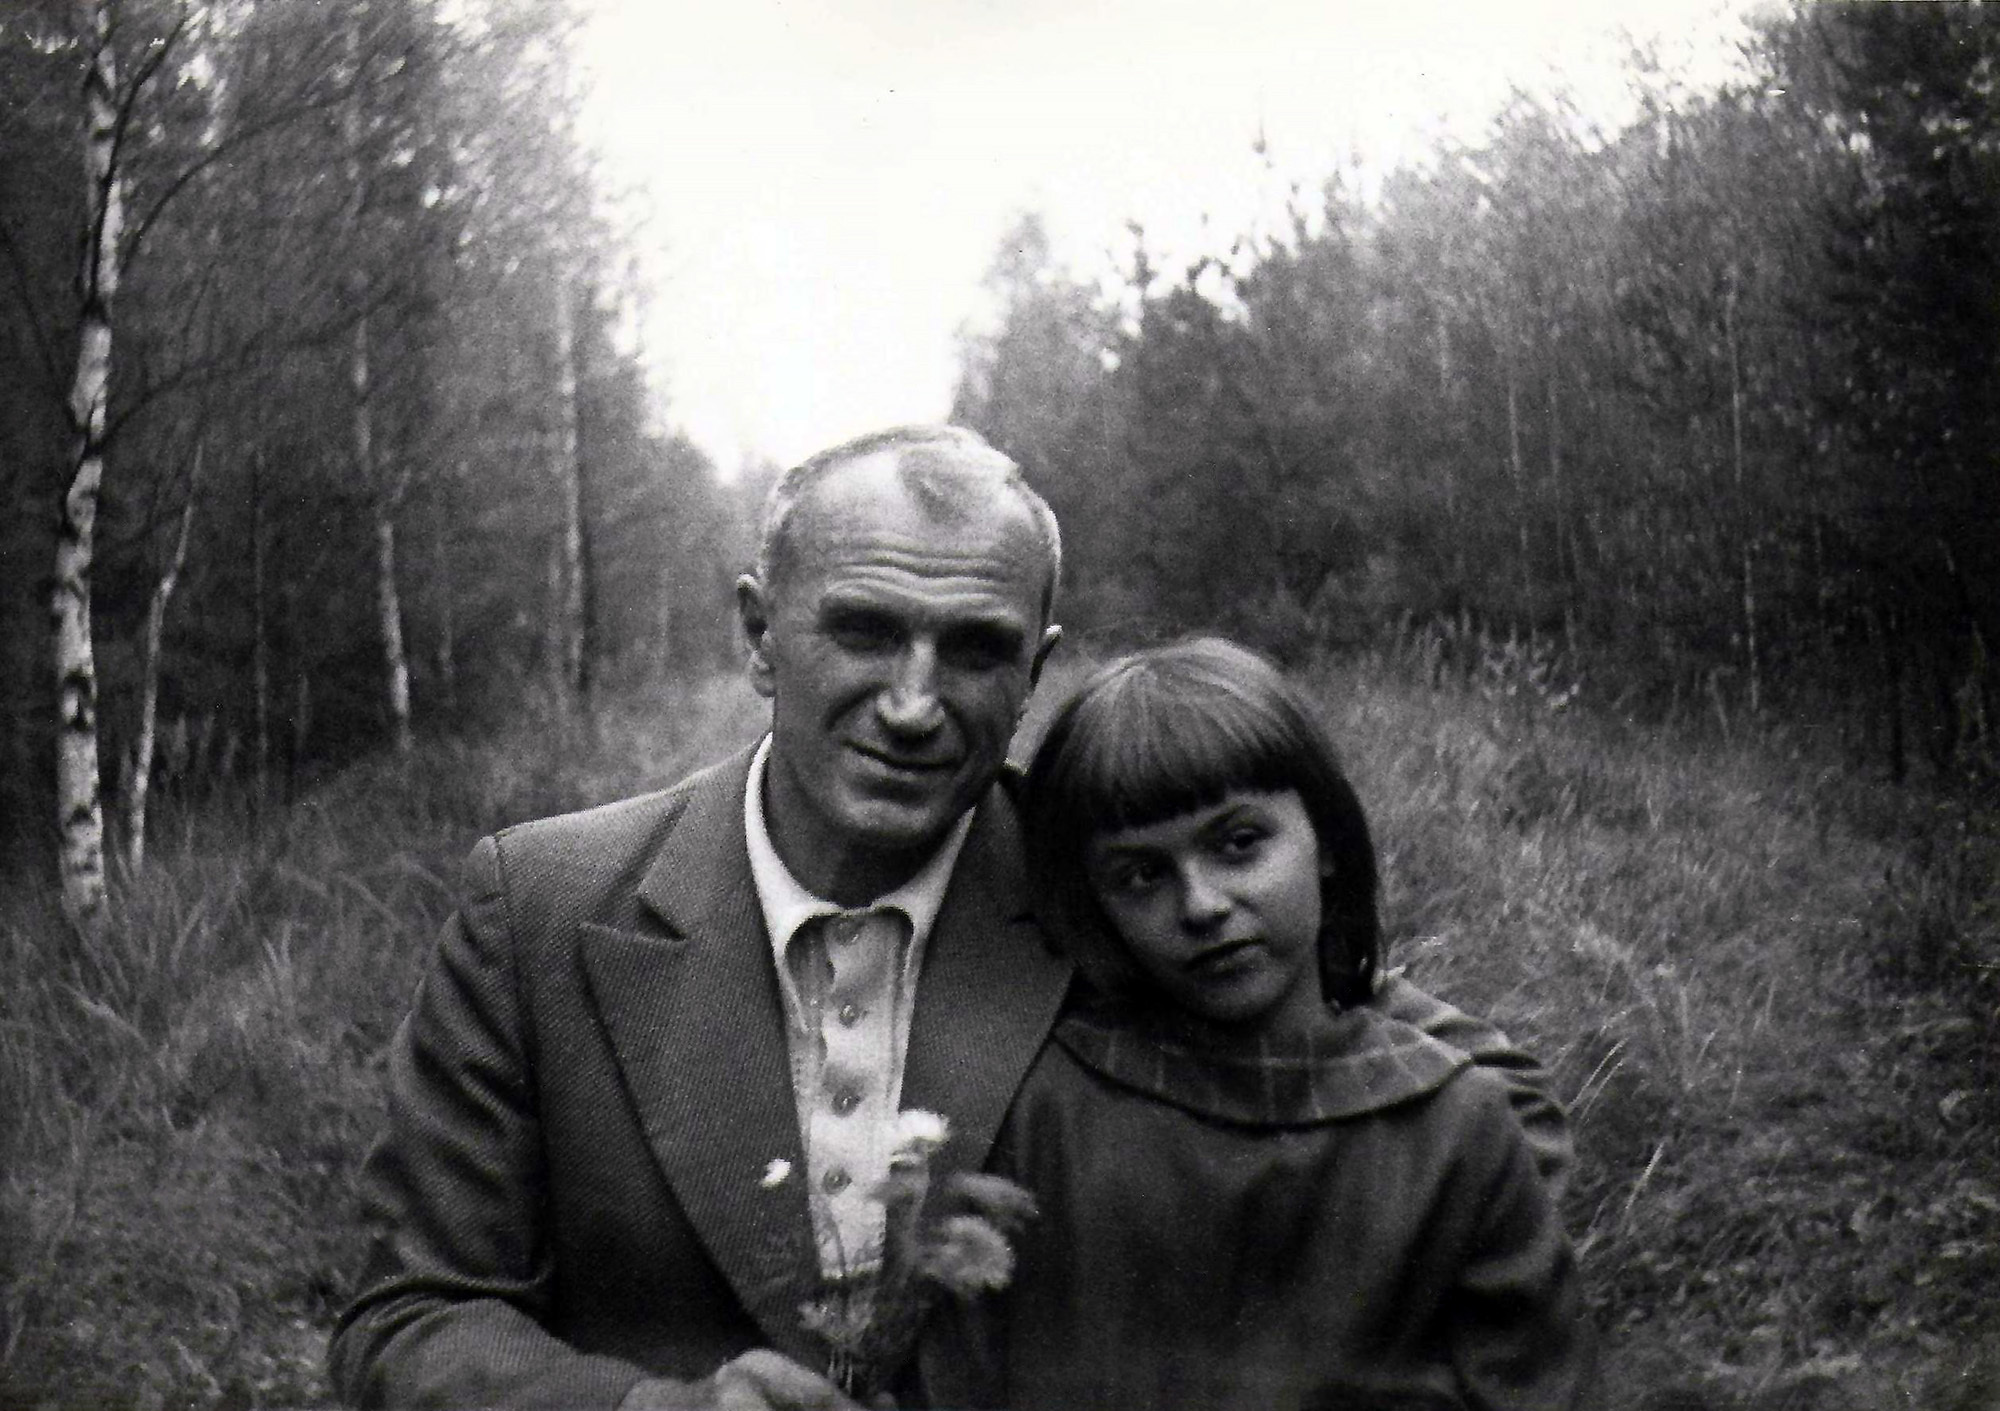
\includegraphics[width=3.65in,scale=1]{img/Mom_Grandpa_Old_small.jpg}}}
\AddToShipoutPicture*{\hspace{0cm}\put(305,63.5){\textcolor{DarkBlue}{\textit{A short study in symmetries across time and space.}}}}

%\bigquote{de nuestras plantas actúan como pantalla frente a los ruidos exteriores e interiores, sobre todo en lugares pequeños y cerrados.}

\end{article*}


\begin{article*}
\invisiblesection{Meditations}


\AddToShipoutPicture*{\put(15,435){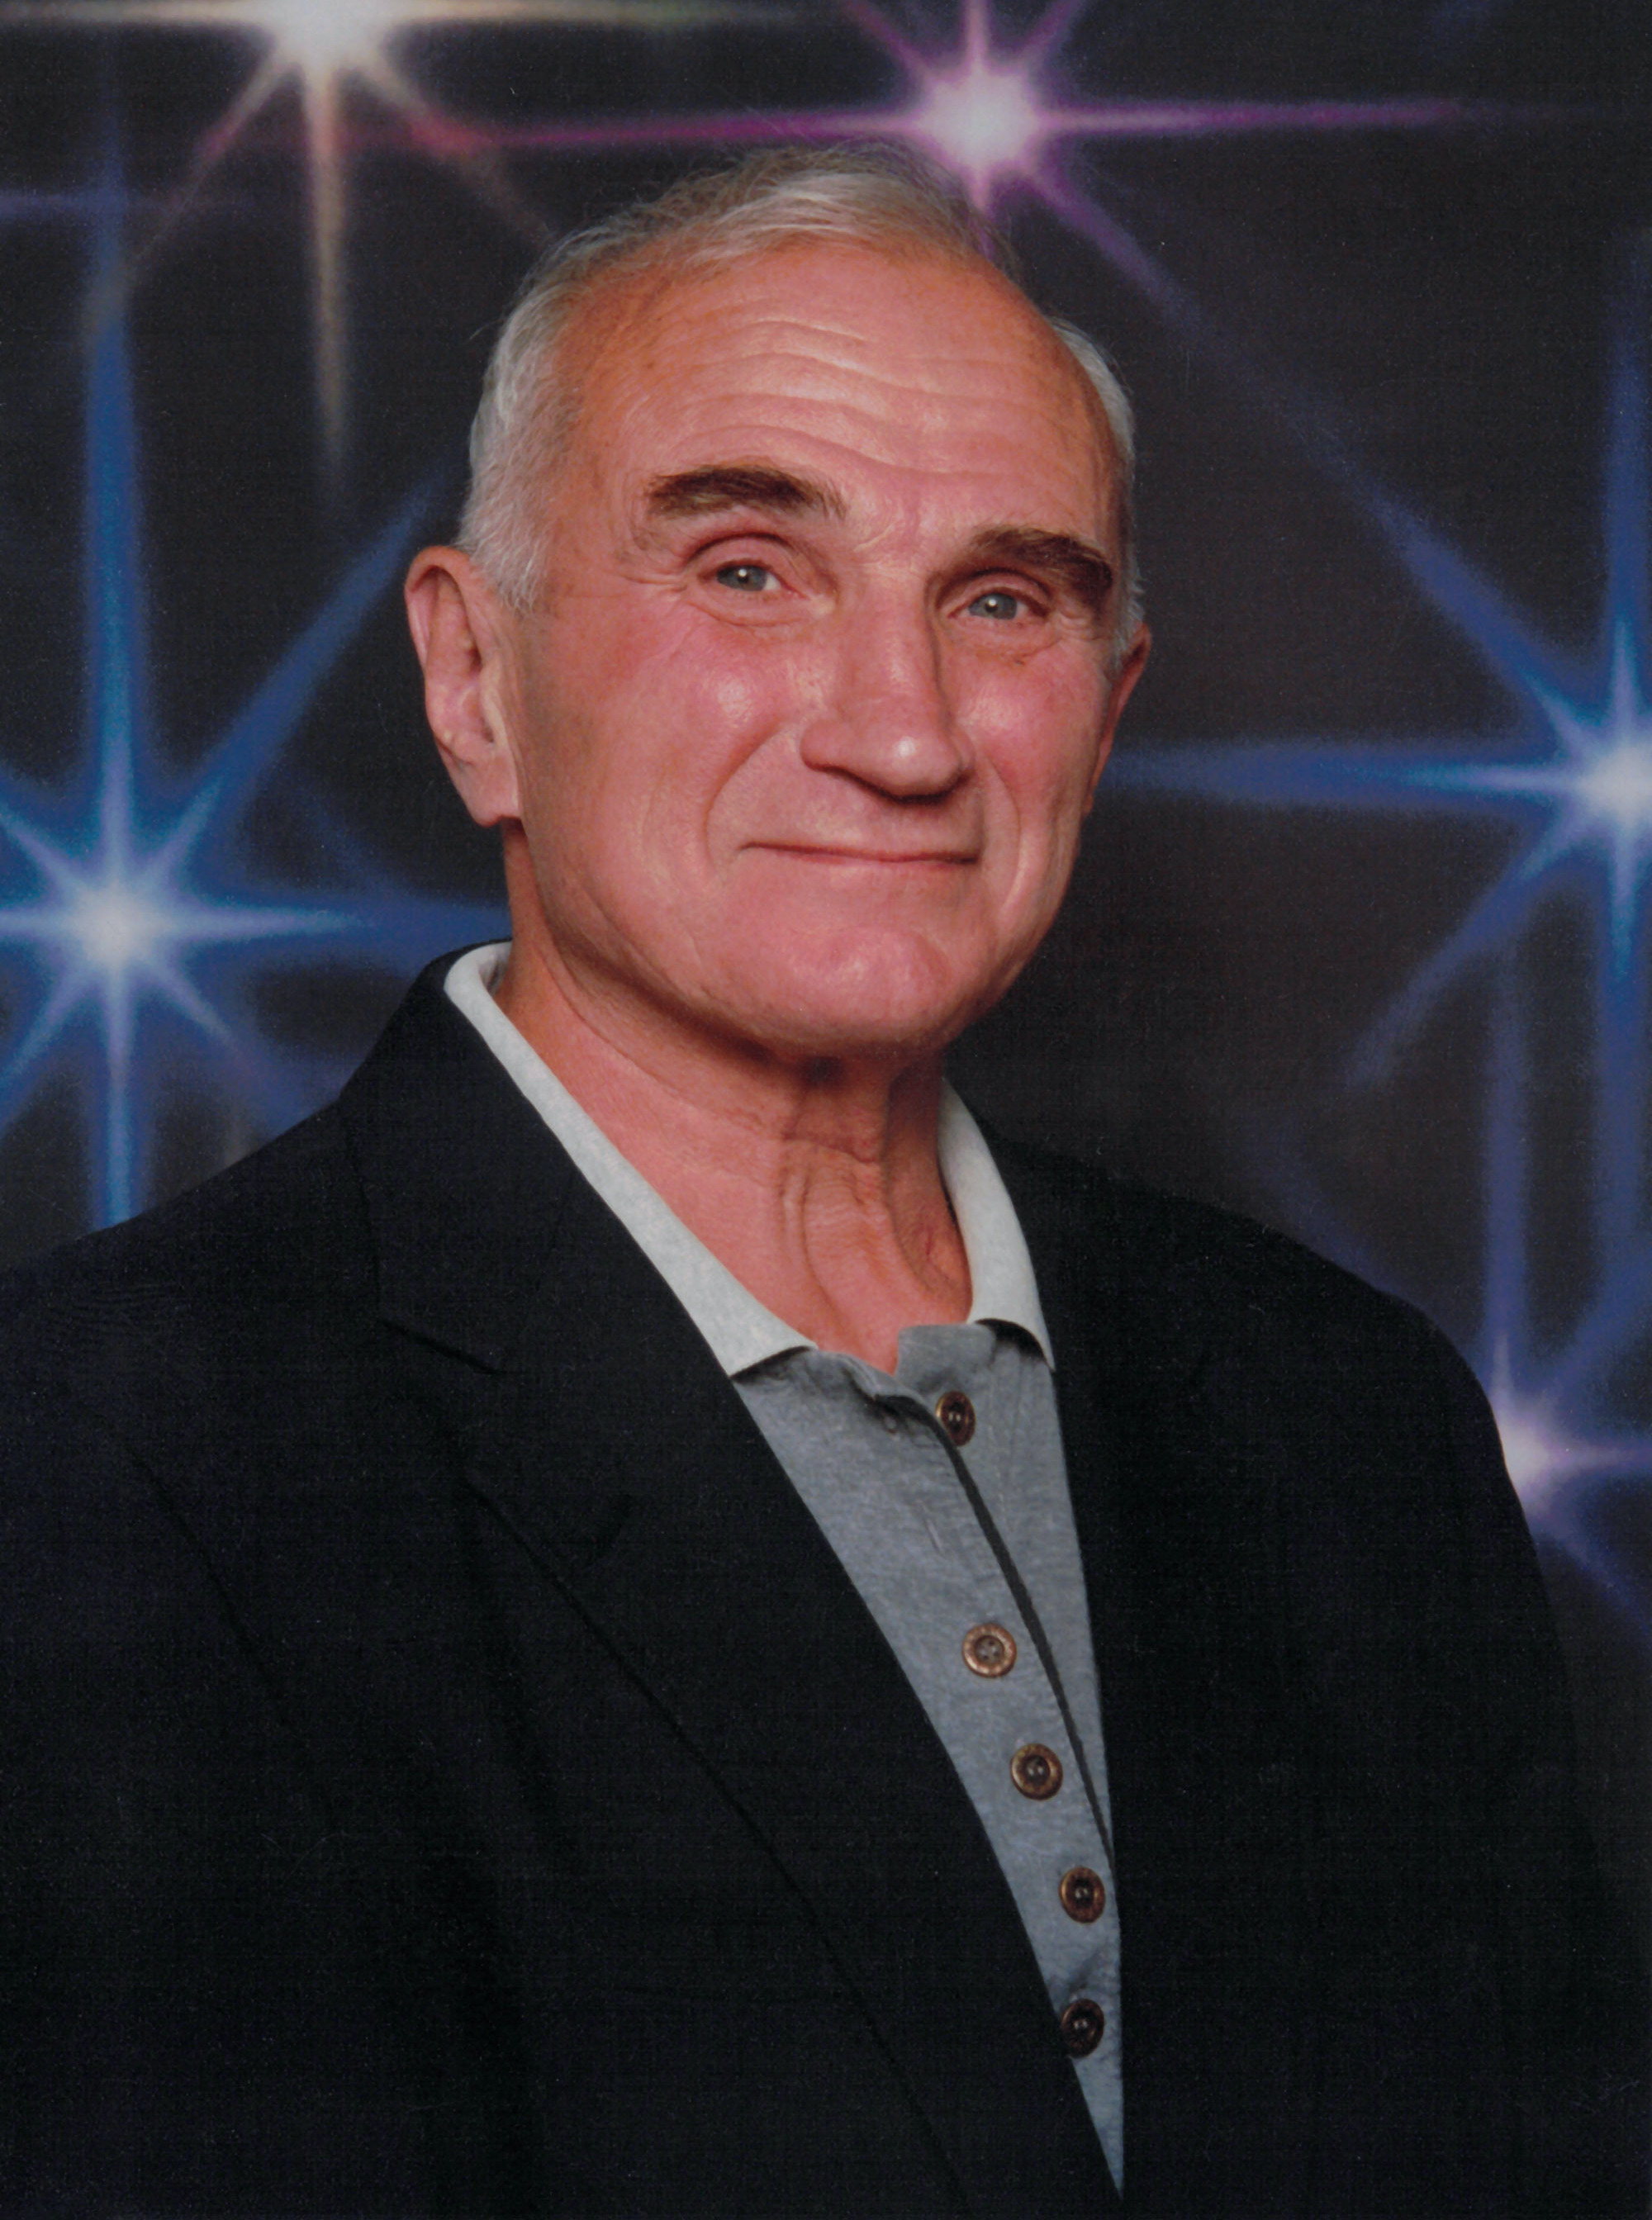
\includegraphics[width=3.2in,scale=1]{img/highschool_gpa_small.jpg}}}
\AddToShipoutPicture*{\put(15,425){\textcolor{DarkBlue}{\textit{Getting ready for high-school prom.}}}}
\AddToShipoutPicture*{\put(15,265){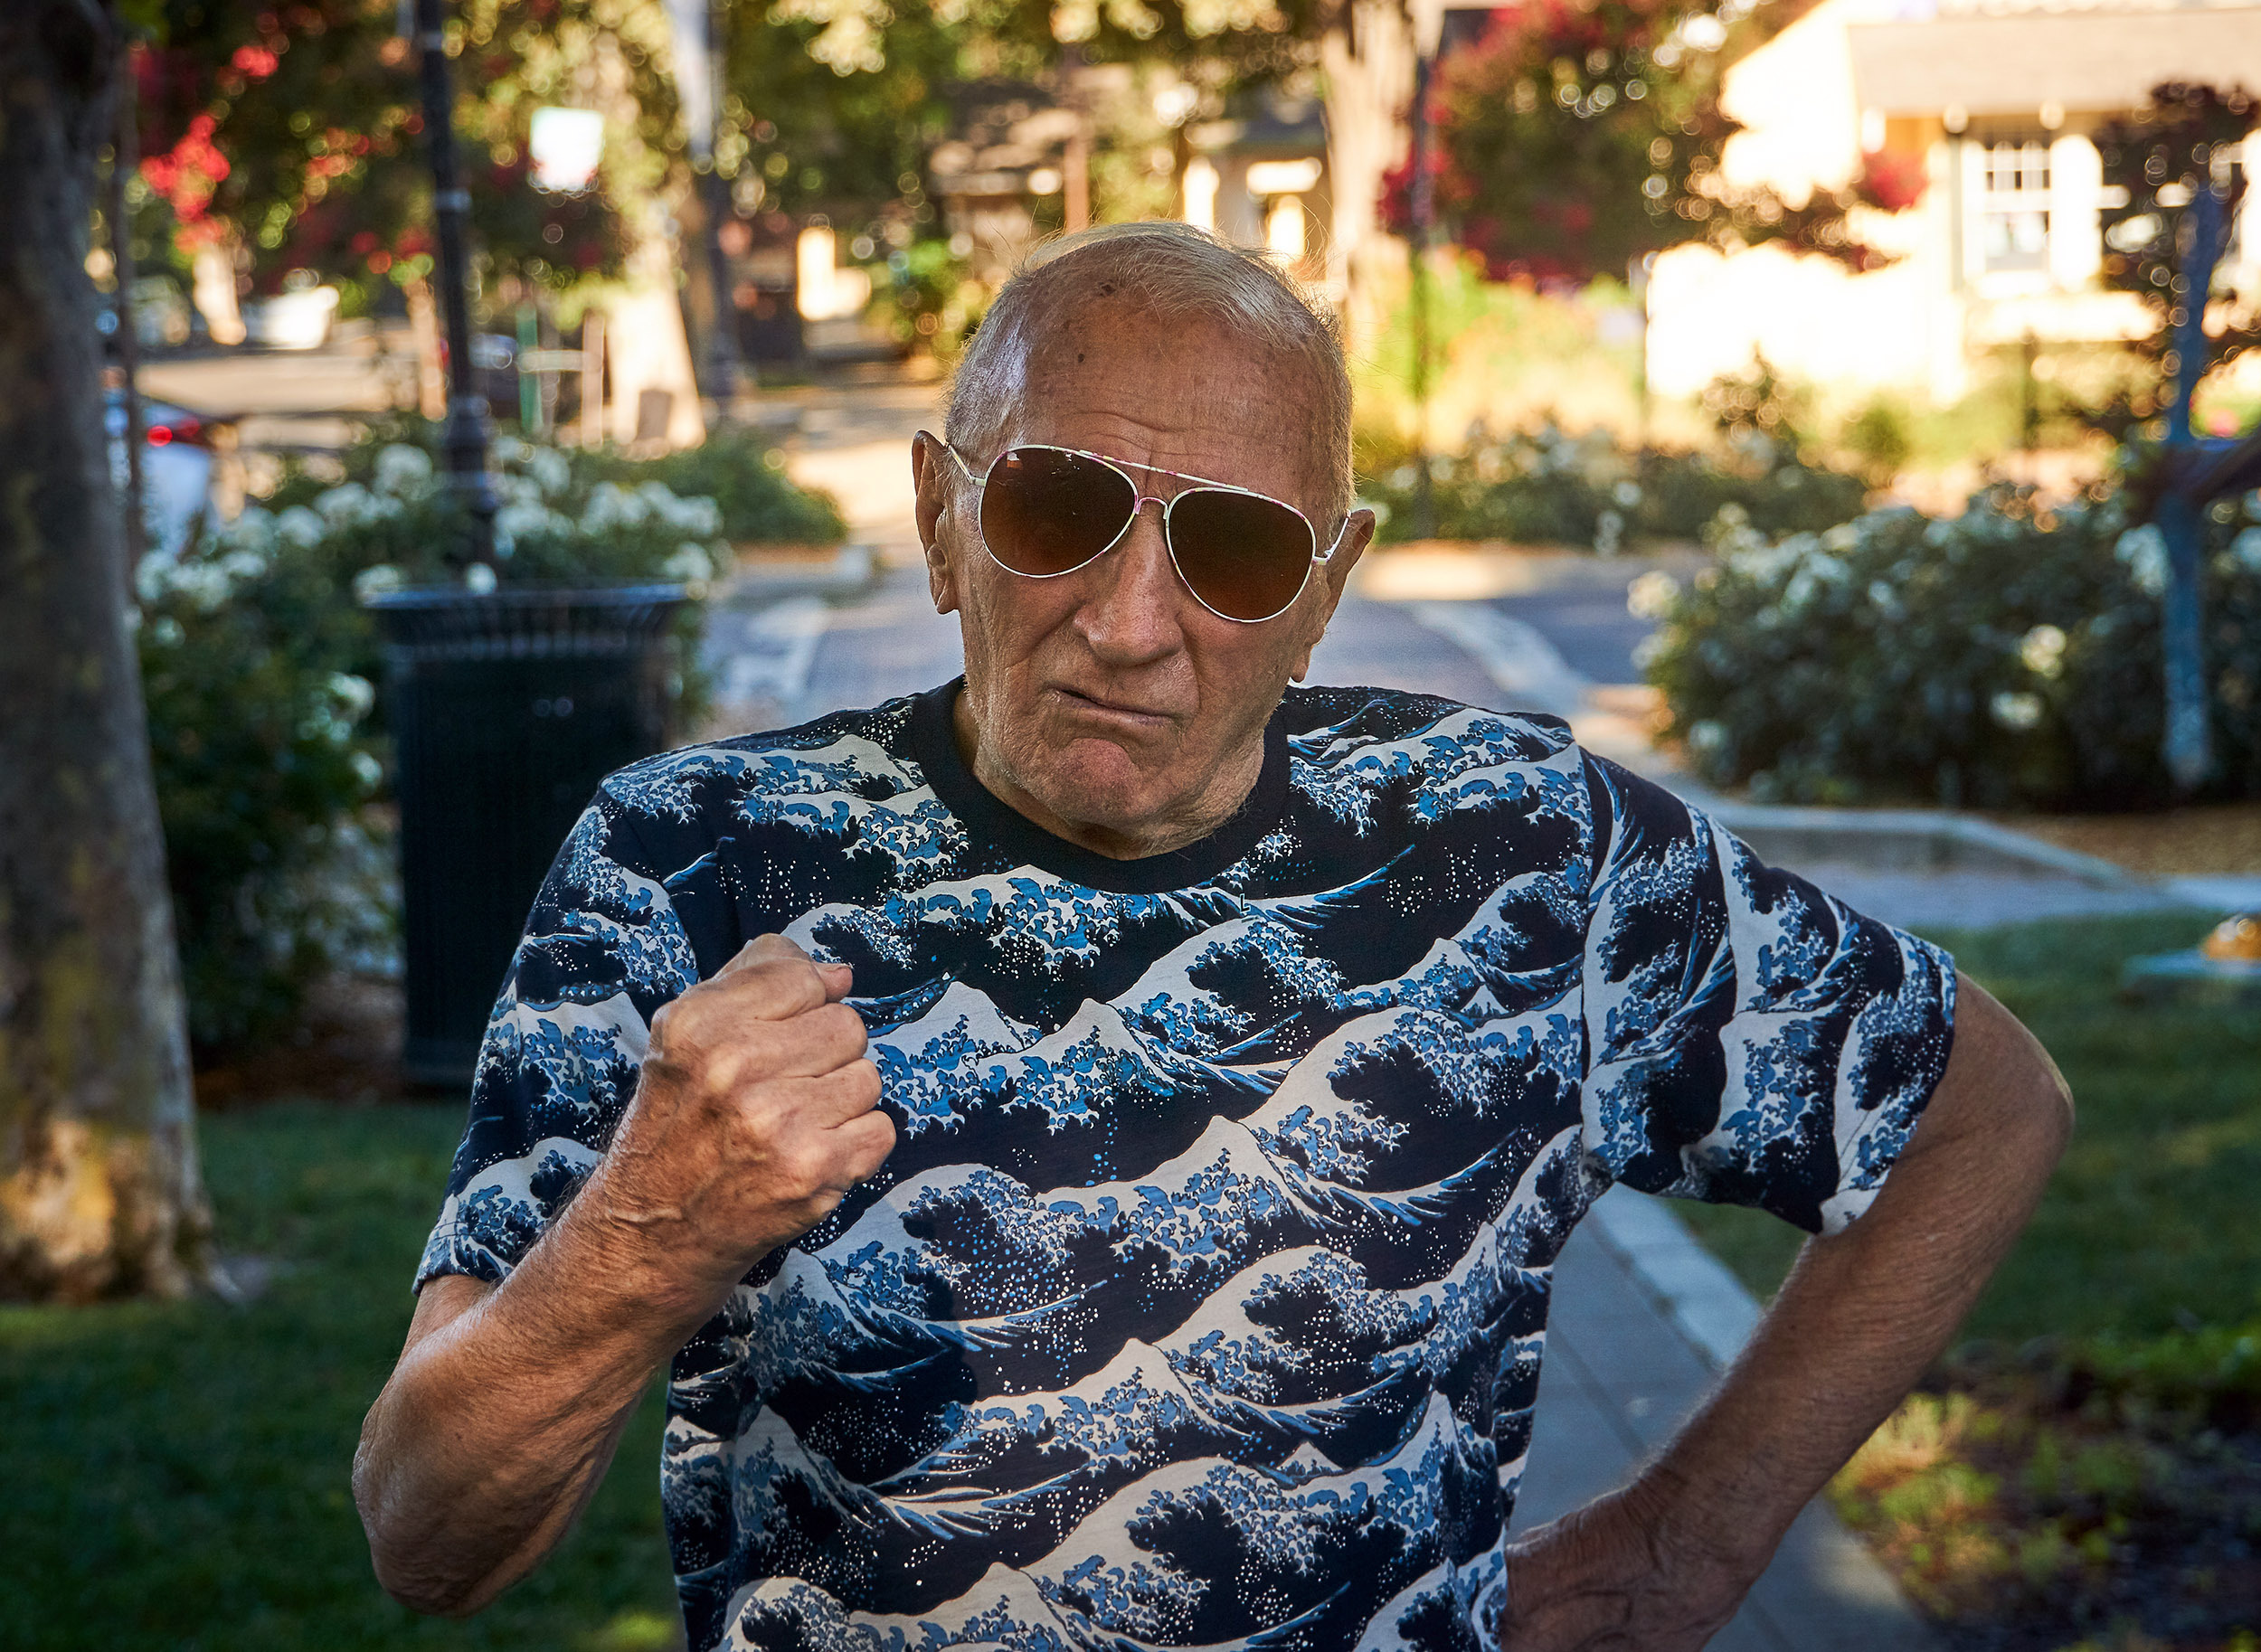
\includegraphics[width=2.775in,scale=1]{img/toughGrandpa.jpg}}}
\AddToShipoutPicture*{\put(15,255){\textcolor{DarkBlue}{\textit{Possible anger at this reflection?}}}}
\AddToShipoutPicture*{\put(15,30){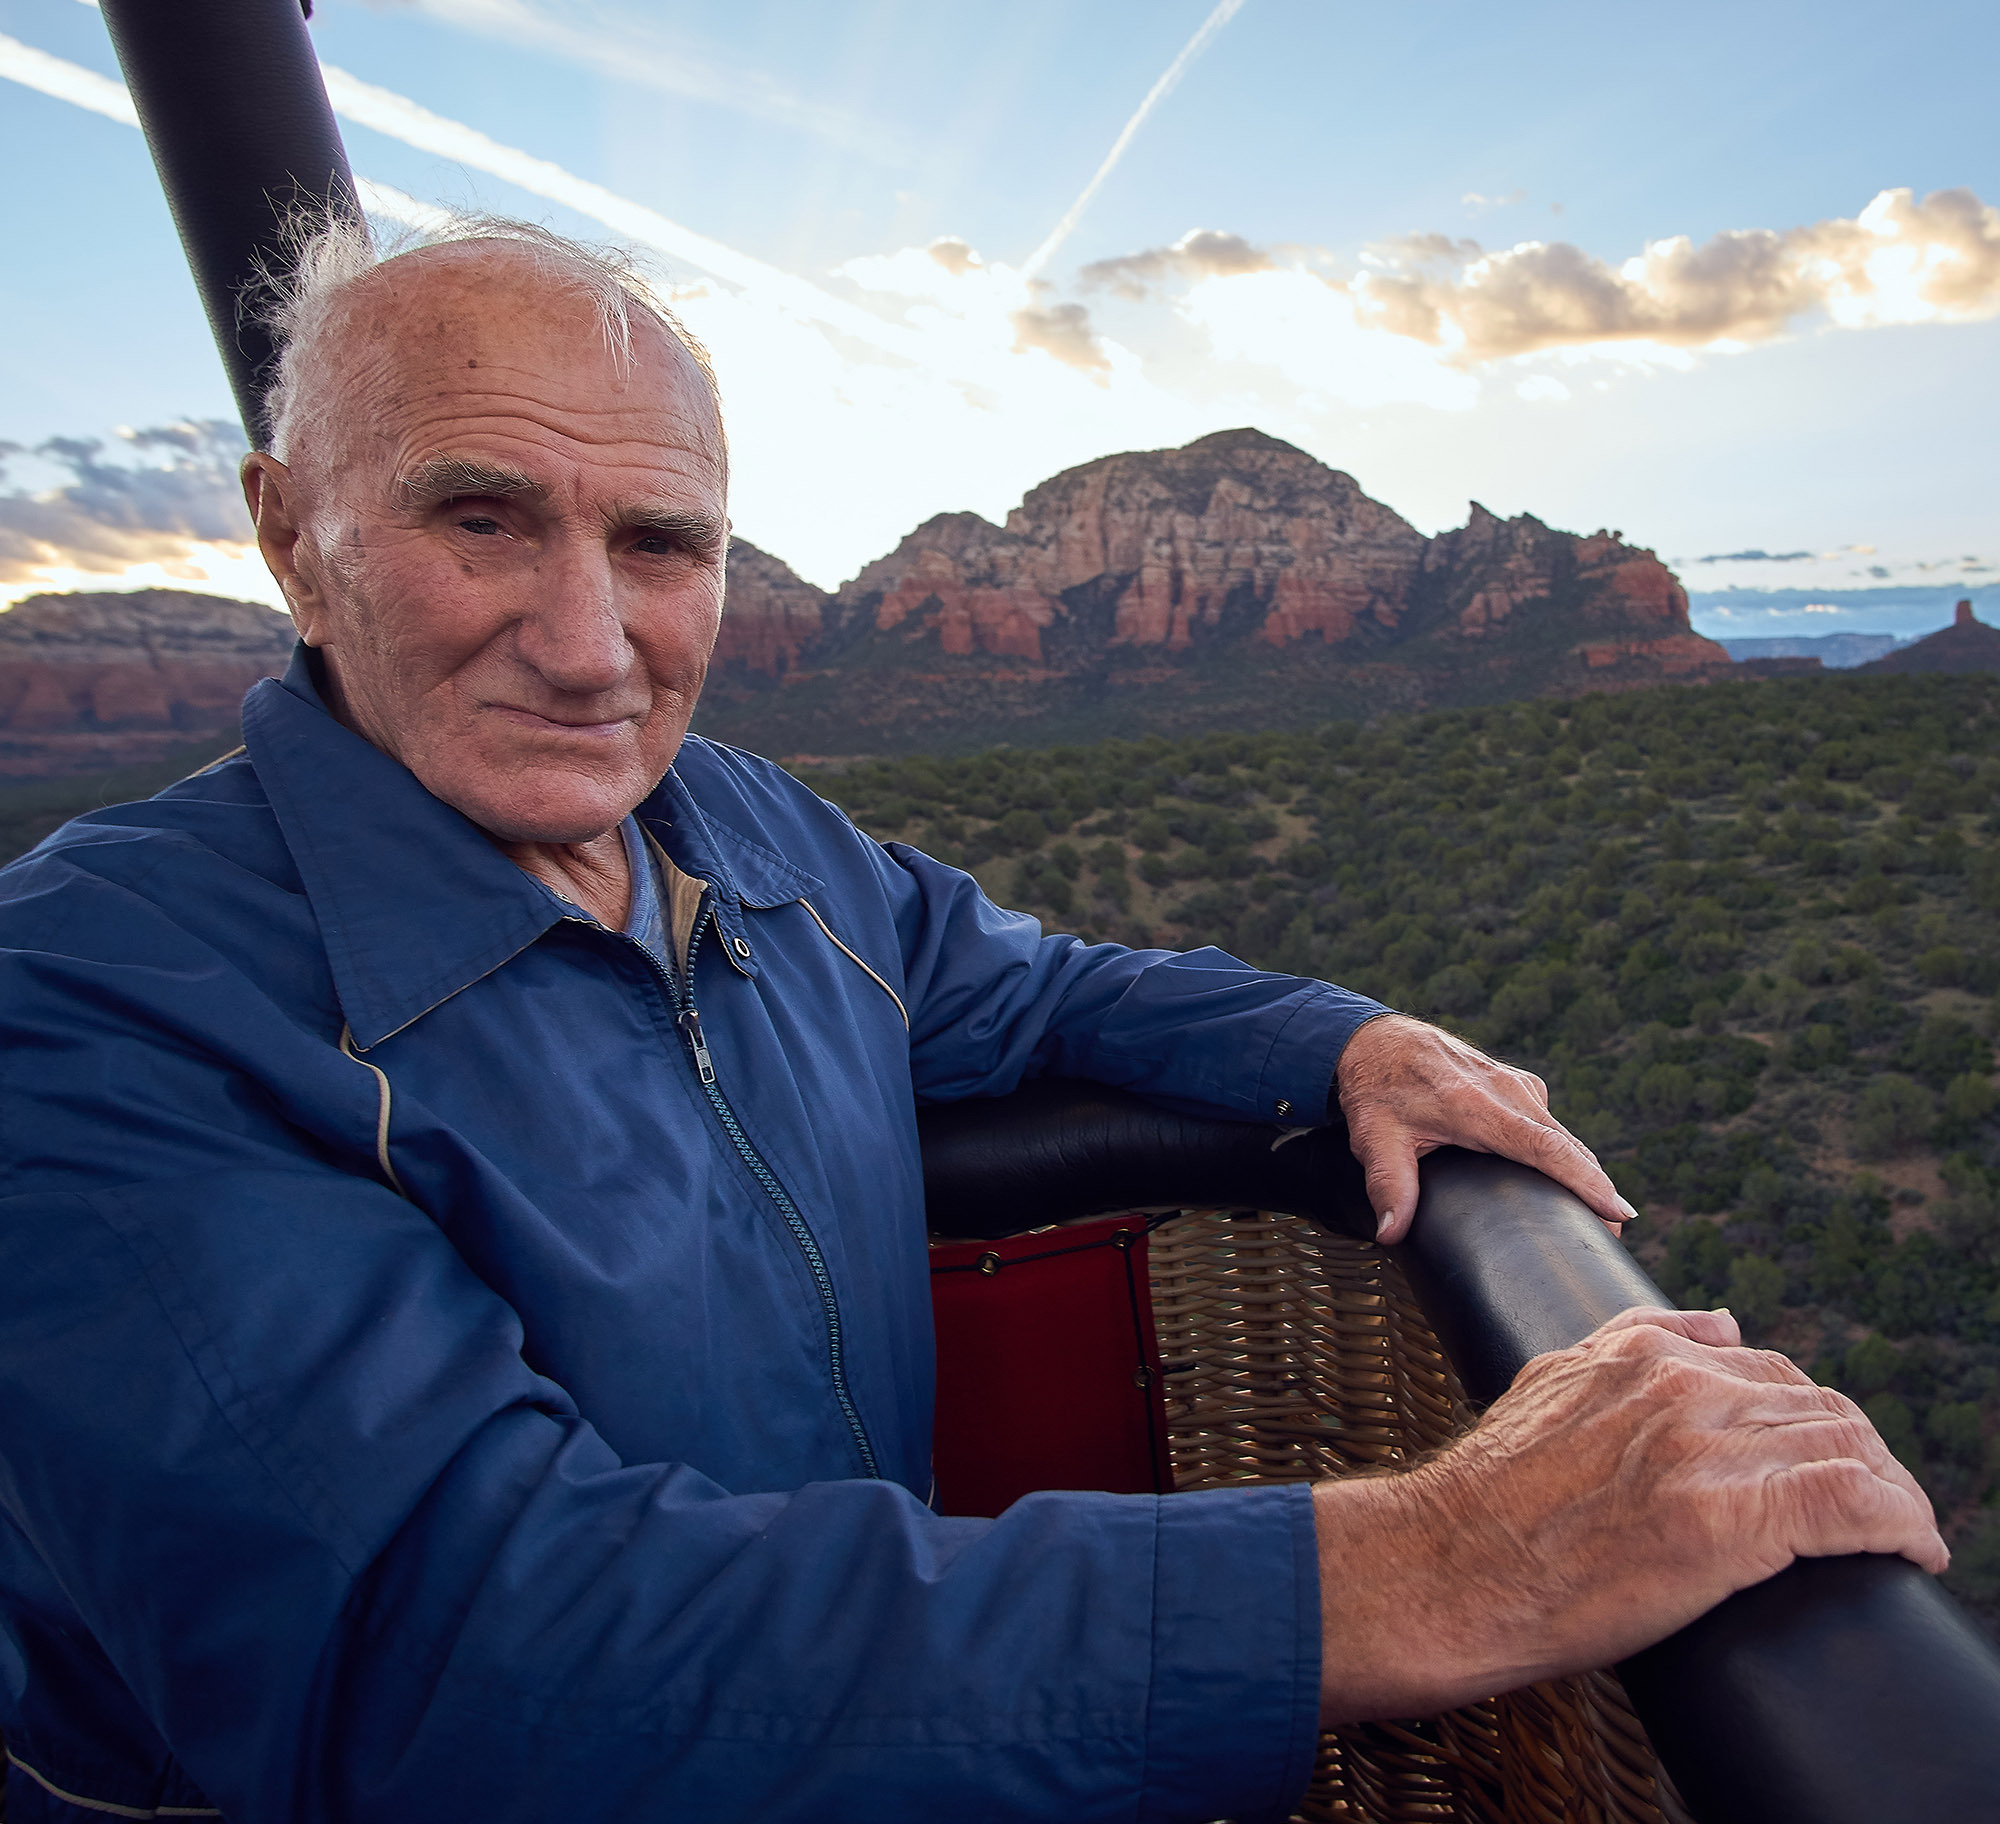
\includegraphics[width=3.2in,scale=1]{img/grandpaHotAirBalloon2.jpg}}}
\AddToShipoutPicture*{\put(15,20){\textcolor{DarkBlue}{\textit{Coupled with its natural partner, skepticism.}}}}
\AddToShipoutPicture*{\put(215,51.5){
\includegraphics[width=1.5in, height=8.8in,scale=1]{img/white.png}}}


\lettrine{Y}{} esterday morning at 5:30 AM my grandfather died, and a part of me died with him. 
\\\\
This is straightforwardly implied by the union of my thoughts on \href{https://nikvetr.wordpress.com/2016/02/23/what-is-love/}{love} and \href{https://nikvetr.wordpress.com/2016/10/26/who-am-i/}{personal identity}. But I also believe through their lens can be seen some small solace in matters of life and death. Certainly, my views in this matter are not especially well-developed or robust – amateur philosophizing rarely holds to the standards of proper scrutiny, and I myself have received remarkably little formal training in the fields of metaphysics, axiology, or anything else relevant. Perhaps the only outcome of these sophomoric ramblings is the erection of flimsy, convoluted phantasm.
\\\\
\tikzoverlay[text width=10in] at (0.75in,4.35in) {
  \LARGE{A Brief Meditation on \textcolor{DarkRed}{Death}}
};
With that disclaimer behind us, to quickly recap: my position is that the essential- and inner-most kernel of an individual’s being, of their personal identity, is contained in their preferences: their weighing of world-states according to those which they’d most work to instantiate, and those which they’d most work to prevent. Their conatus, in other words, or their utility functions, to dress the idea in somewhat nerdier cloth. Fleeting thoughts, feelings, dispositions, memories, knowledge, and appearances (or even their temporal continuity) come secondary, all serving as vehicles to exact their wills upon the world, with the most obvious vehicle being that meat puppet they pilot around and direct towards this end or that. When considering possible worlds distinguished only by changes in some aspect of \textit{me}, I balk most strongly at those featuring the modification of my core values and preferences – implant new memories, transplant my brain, or induce however many secondary changes to my sense of aesthetics or taste in frivolities, but make me love those I hate and hate those I love, and I shall be destroyed as surely as anything. 
\\\\
(interpersonal love and hate, as described in my own, private language, refer to a mirroring of preferences: any love worth a damn necessarily involves the drive to bring about worlds that your beloveds themselves prefer)
\\\\
In this view, a person’s identity primarily exists as a causal impetus to satisfy some particular pattern of preferences, and manifests externally insofar as the trajectory of the world deviates from whatever alternative trajectory may have been generated in their absence. This force can be distributed within the substrate that directly describes it (e.g. that squishy organ residing in one’s head), within copies of itself inside other substrates, or within structures even further afield that we, through our actions, create and cause to perpetuate themselves under their own power. So long as my will be done to equal effect, I am largely impartial to the exact mechanism according to which it is satisfied, at least if that will does not pertain to the exact form of that mechanism. So long as the world is different with my passing through it, the pattern of my will remains. And insofar as I bring into the world entities that counterfactually perpetuate my will, that exist to guide the future into states I prefer – insofar as my identity is primarily defined by the multitudinous set of my preferences – those entities may remain as extensions of myself, even as the primary vehicle by which will is realized (my body and mind) ceases to function. Those external structures are subsumed into myself as a distributed network of causal drives according to which I’m defined. Death becomes as nothing before the fulfillment of ambition, at least in principle.
\\\\
(I should note that in these mental convolutions I remain as staunchly physicalist – or at least some flavor substance monist – as ever. Accommodating uncertainty as best I’m able, I hold there is no spooky, irreducible ghost interfacing with the physical world, and any talk of wills or utility functions refers to an emergent property of molecular patterns that further supervene on what we see around us. I should also note that this perspective is quite distinct from that which posits that someone never dies so long as they’re kept alive in living memory. That would only apply here so long as their principal desires were to be remembered; otherwise, if those memories evoke no calls to action, a purely mnestic existence conjures only a pale shadow of the departed’s former selves. Neither would I ever consider Bymba to be the thousand winds that blow – he was only ever but the one)
\\\\
(it is also this metaphysic that helps me to reconcile my own fondness for preference utilitarianism with a respect for the wishes of the dead — though as elsewhere, plenty of unintuitive corner cases are quick to arise. But I still find it more intuitive than appeals to social contracts or retro-causal justifications for benefitting or harming the so-called \textit{non-existent})
\\\\
Difficulties arise when the will is largely self-affecting. If the majority of one’s preferences are directed towards the sustenance of one’s body or the valence of personal, hedonic experiences, then the death of that body will indeed see one’s identity greatly reduced. To the extent one’s preferences are self\textit{less}, however, they can continue to be satisfied long after flesh has sloughed off bones and bones have been ground to dust. Bymba held many ambitions throughout his life, and several of them – especially a personal trip to the planet Mars, which he’d played a major role in planning prior to the fizzling of the 20th century’s space race – went unfulfilled. And upon his death he never left behind any far-reaching quest to rid the world of battery-farm hens or malaria. But in his final decades, his thoughts and actions were quite singular in their purpose: to ensure that we, his friends and family, flourished in our own trips along the mortal coil. He charged us to live well, to not neglect to care for ourselves and others, to love those around us. And so long as we strive to carry out those desires, a major part of him may yet survive.
\\

\AddToShipoutPicture*{\put(365,500){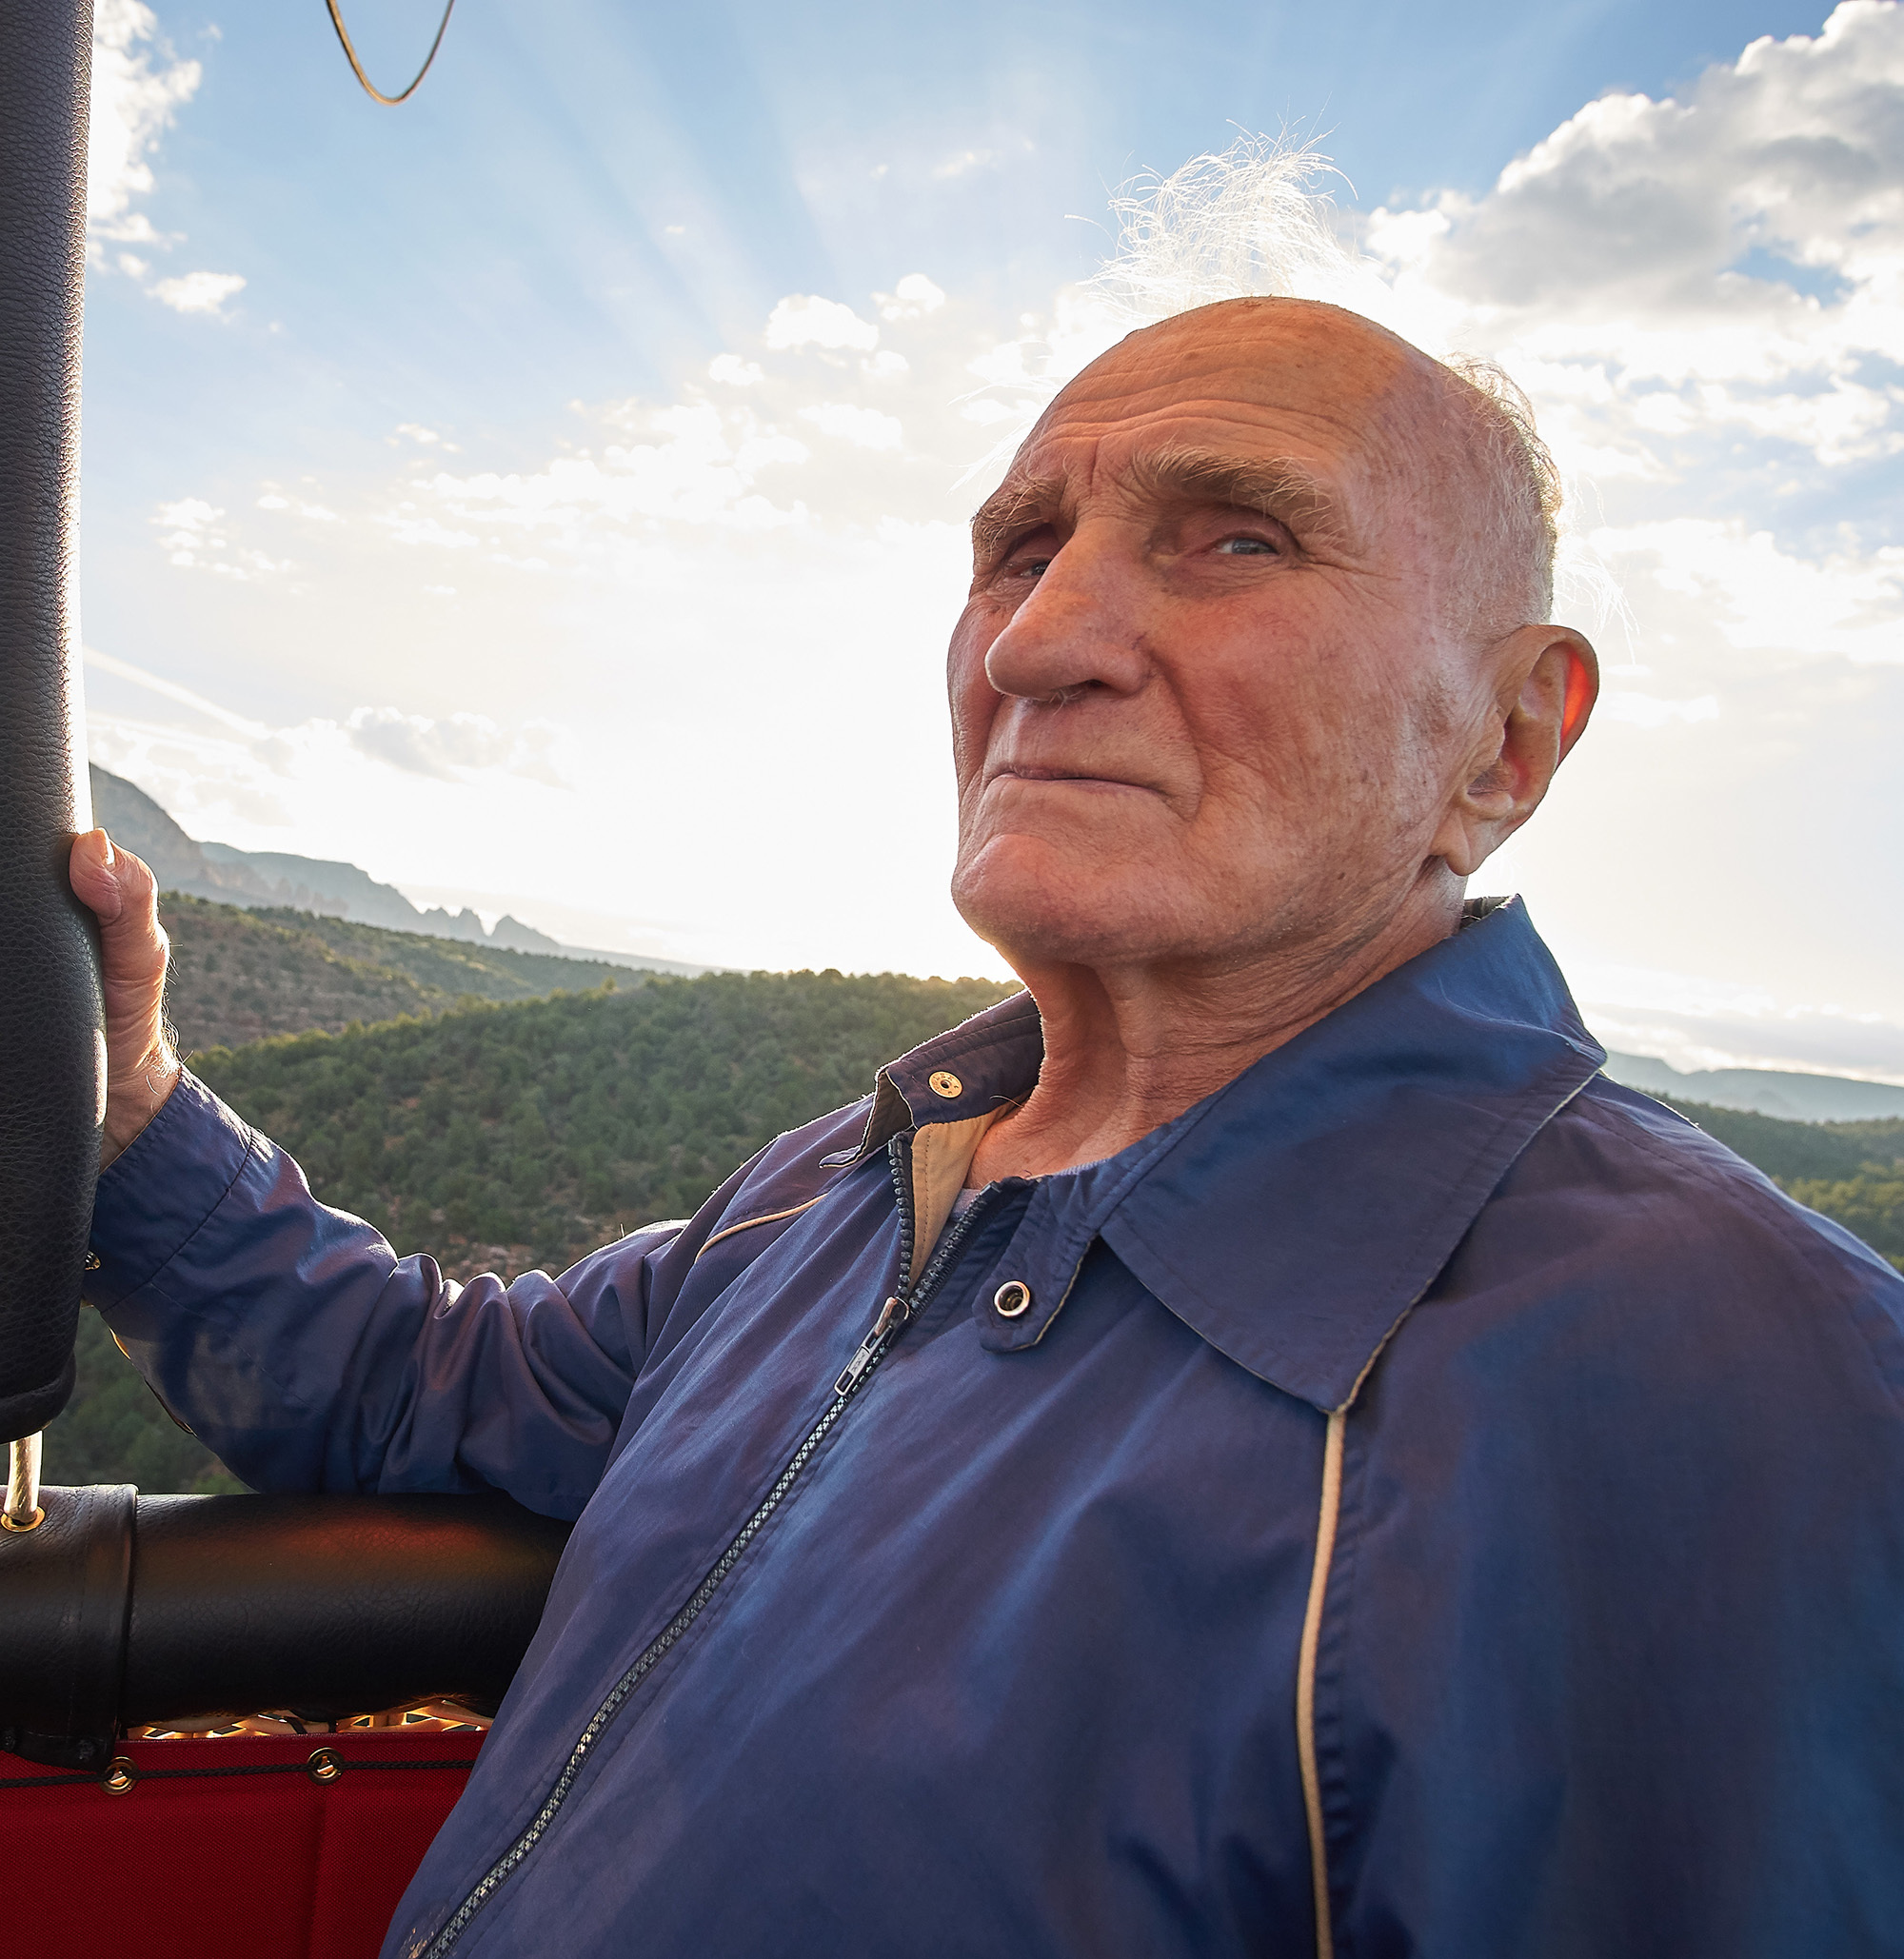
\includegraphics[width=3.25in,scale=1]{img/grandpaHotAirBalloon3.jpg}}}
\AddToShipoutPicture*{\put(490,490){\textcolor{DarkBlue}{\textit{Something is clearly amiss.}}}}
\AddToShipoutPicture*{\put(400,170){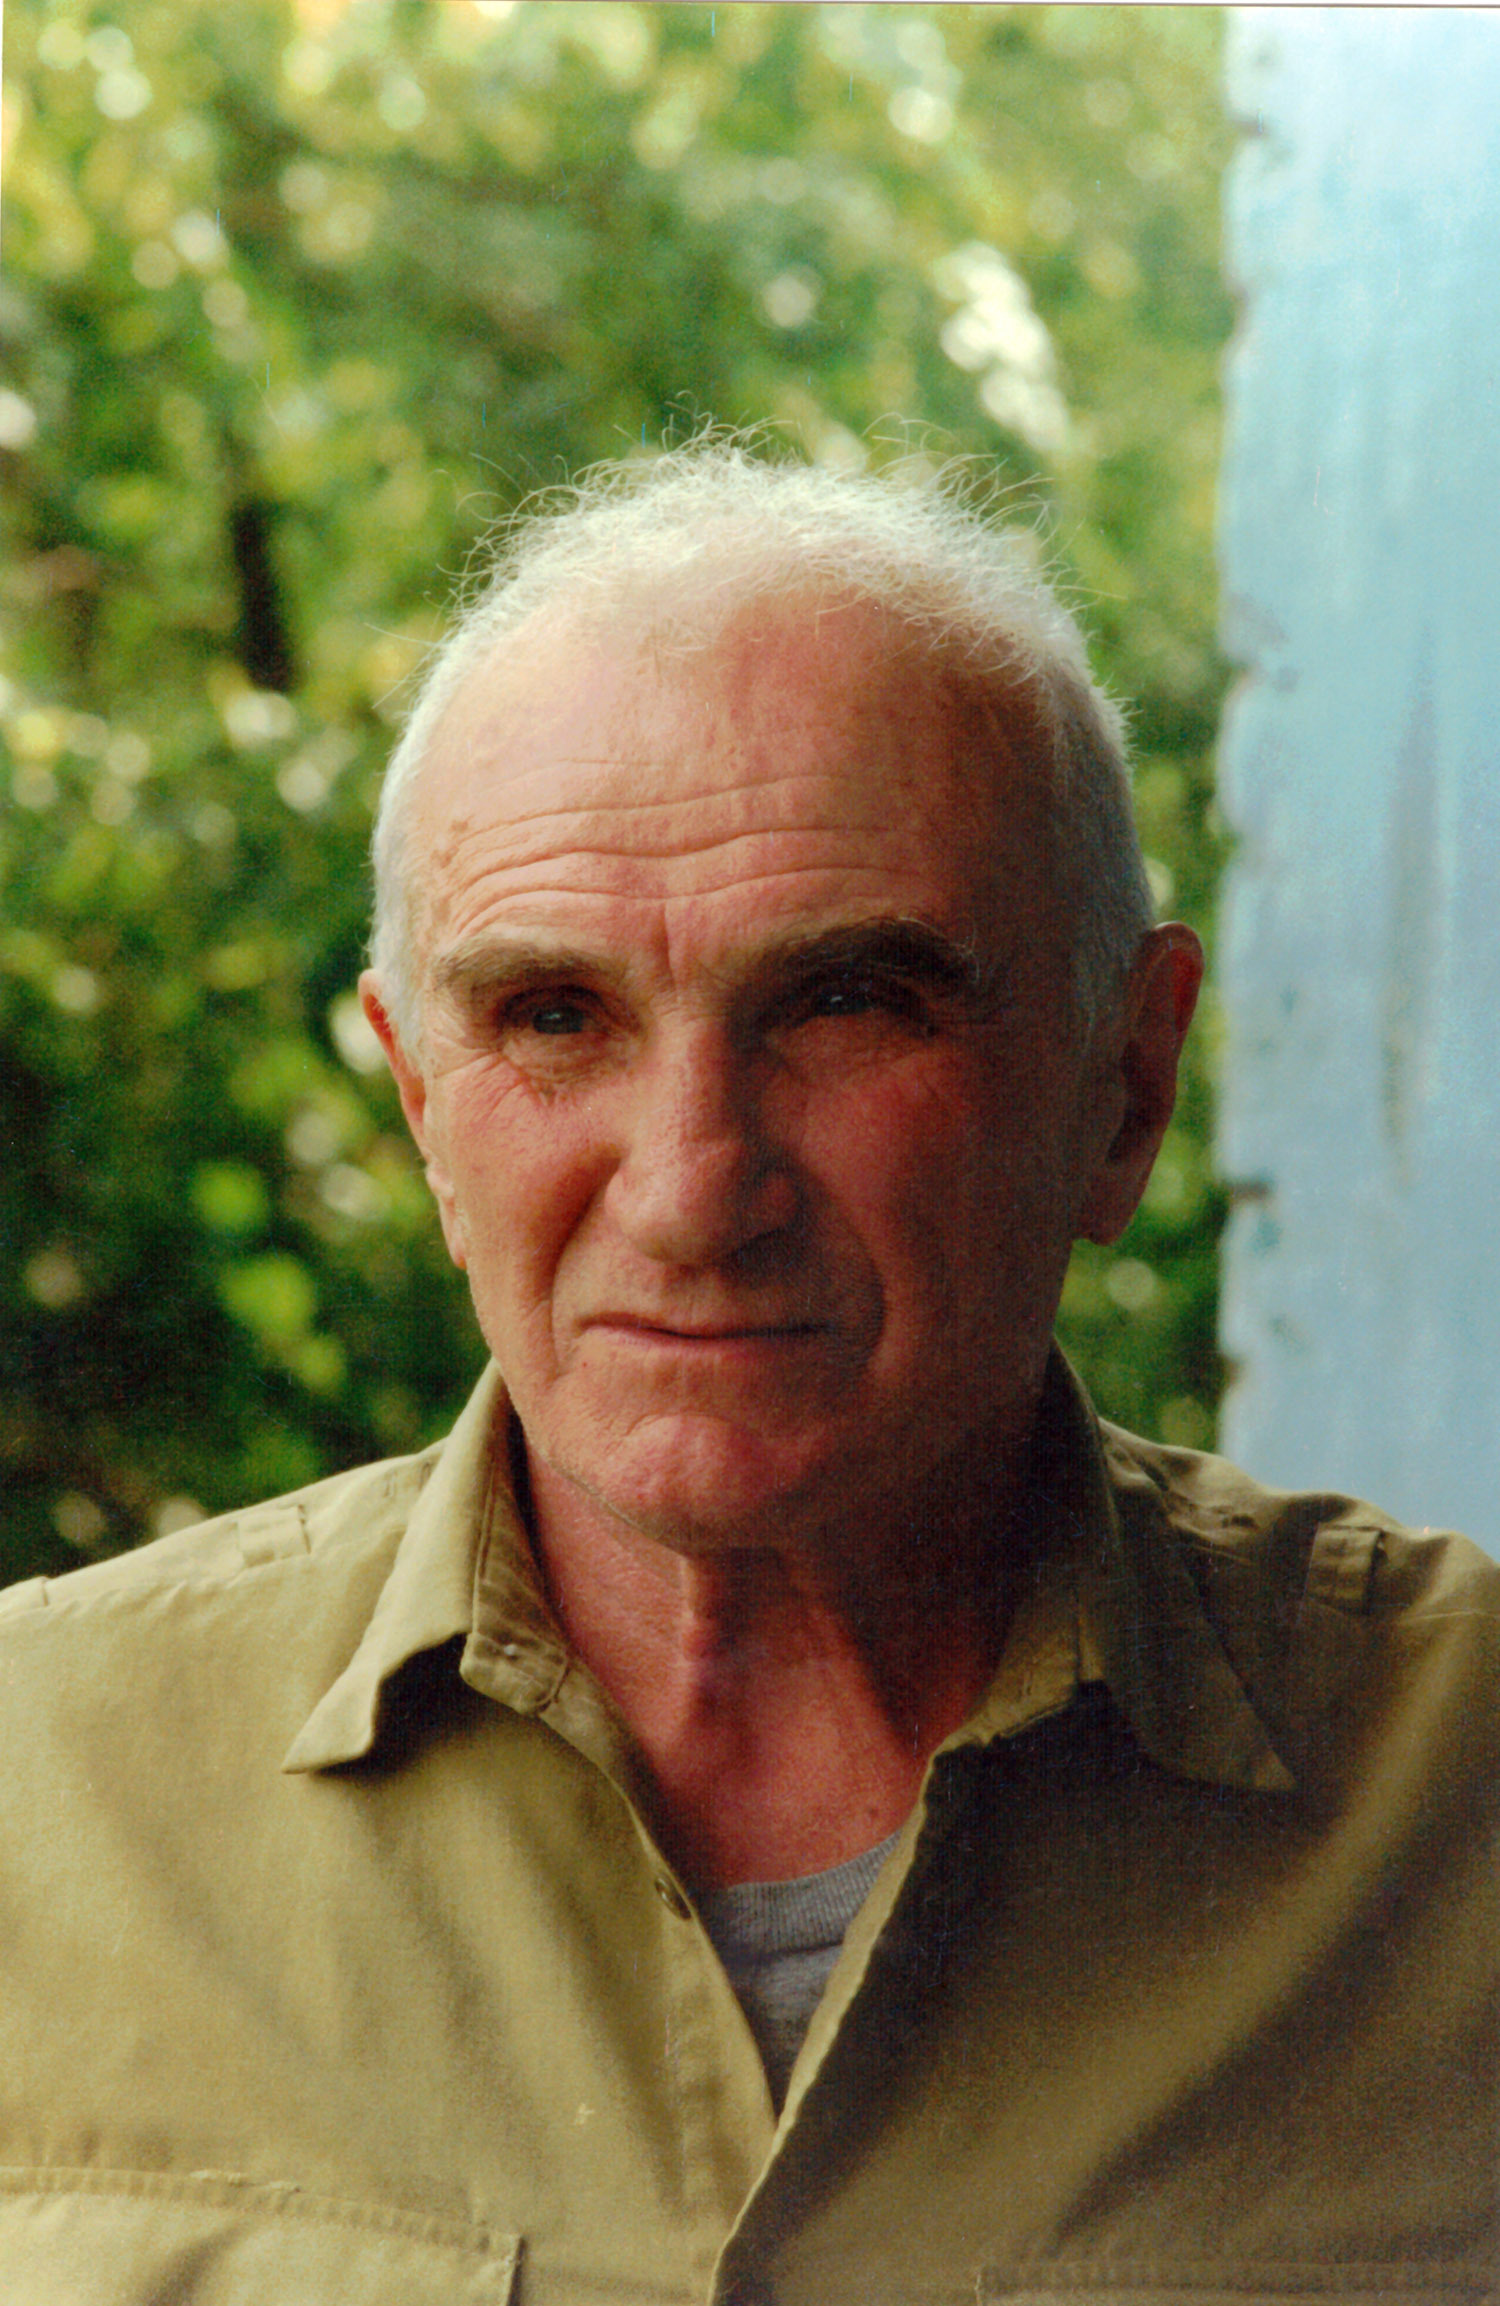
\includegraphics[width=2.75in,scale=1]{img/color_gpa_small.jpg}}}
\AddToShipoutPicture*{\put(445,160){\textcolor{DarkBlue}{\textit{And I think it's this flimsy metaphysic.}}}}
\AddToShipoutPicture*{\put(290,51.5){
\includegraphics[width=1.5in, height=8.8in,scale=1]{img/white.png}}}
%Колюшке на переезд
A small example of such posthumous causal propagation can be seen in an envelope discovered in Bymba’s bedside table while searching for identification to provide the coroner. On it were the words “For Kolia’s move!”, and inside was cash money, in total some \$200. I’d mentioned to him a few weeks prior that we were planning to relocate, and he must quickly have begun to bring his own resources to bear to the extent he was able (for reference, his 2021 pension received in exchange for decades of service to the USSR totalled around \$300 / month). He’d always try to send me money, never taking refusal as an option, much as he’d insist on schlepping a suitcase or two from our car to our rooms during visits, despite barely even managing to stumble around himself. Even as his health failed him, he strove to ease our own movements into the future.
\\\\
In all this one might protest: \textit{awfully} convenient that he might love and be loved in turn, in some reflective dance of mirrored preferences. You have but to do what you’d already meant to in order that a will’s persistence be ensured. But I’d respond that the counterfactual effect of Bymba’s influence may yet differ, with my own actions and preferences conditional on that influence playing out quite differently from those absent that influence. To the extent that I developed the preferences I did in response to an exertion of his will – for example, developing a fondness for the night sky that would certainly have never been had he not dragged me out of bed so often at 3AM – the pattern of his will may still be seen to influence into the future. There might also be a fungibility concern – if grandpa’s causal influence on my preferences shaped them in fully general ways, by instilling in me desire to, say, partake in physical activity, with no great inclination towards one activity or another, then his preferences are only satisfied by my actions in a generic, rather than in any specific sense. These preferences can be said to be quite weak, as their satisfaction is compatible with a great number of possible worlds. In contrast, grandpa certainly desired to be remembered – he’d not have written his memoirs, otherwise – and would doubtless by frustrated by the remembrance of some other, unrelated grandpa. And as causal relation is required here, it is also insufficient for the world to merely drift into states compatible with grandpa’s will, even if through his own actions or their indirect consequences. The exertion needs to result in replicable effect, in a bending of the distribution of possible futures (or perhaps their moments) – it is not enough for states compatible with his preferences to arise by chance, even if coincident with both intention and action.
\\

\AddToShipoutPicture*{\put(-5,0){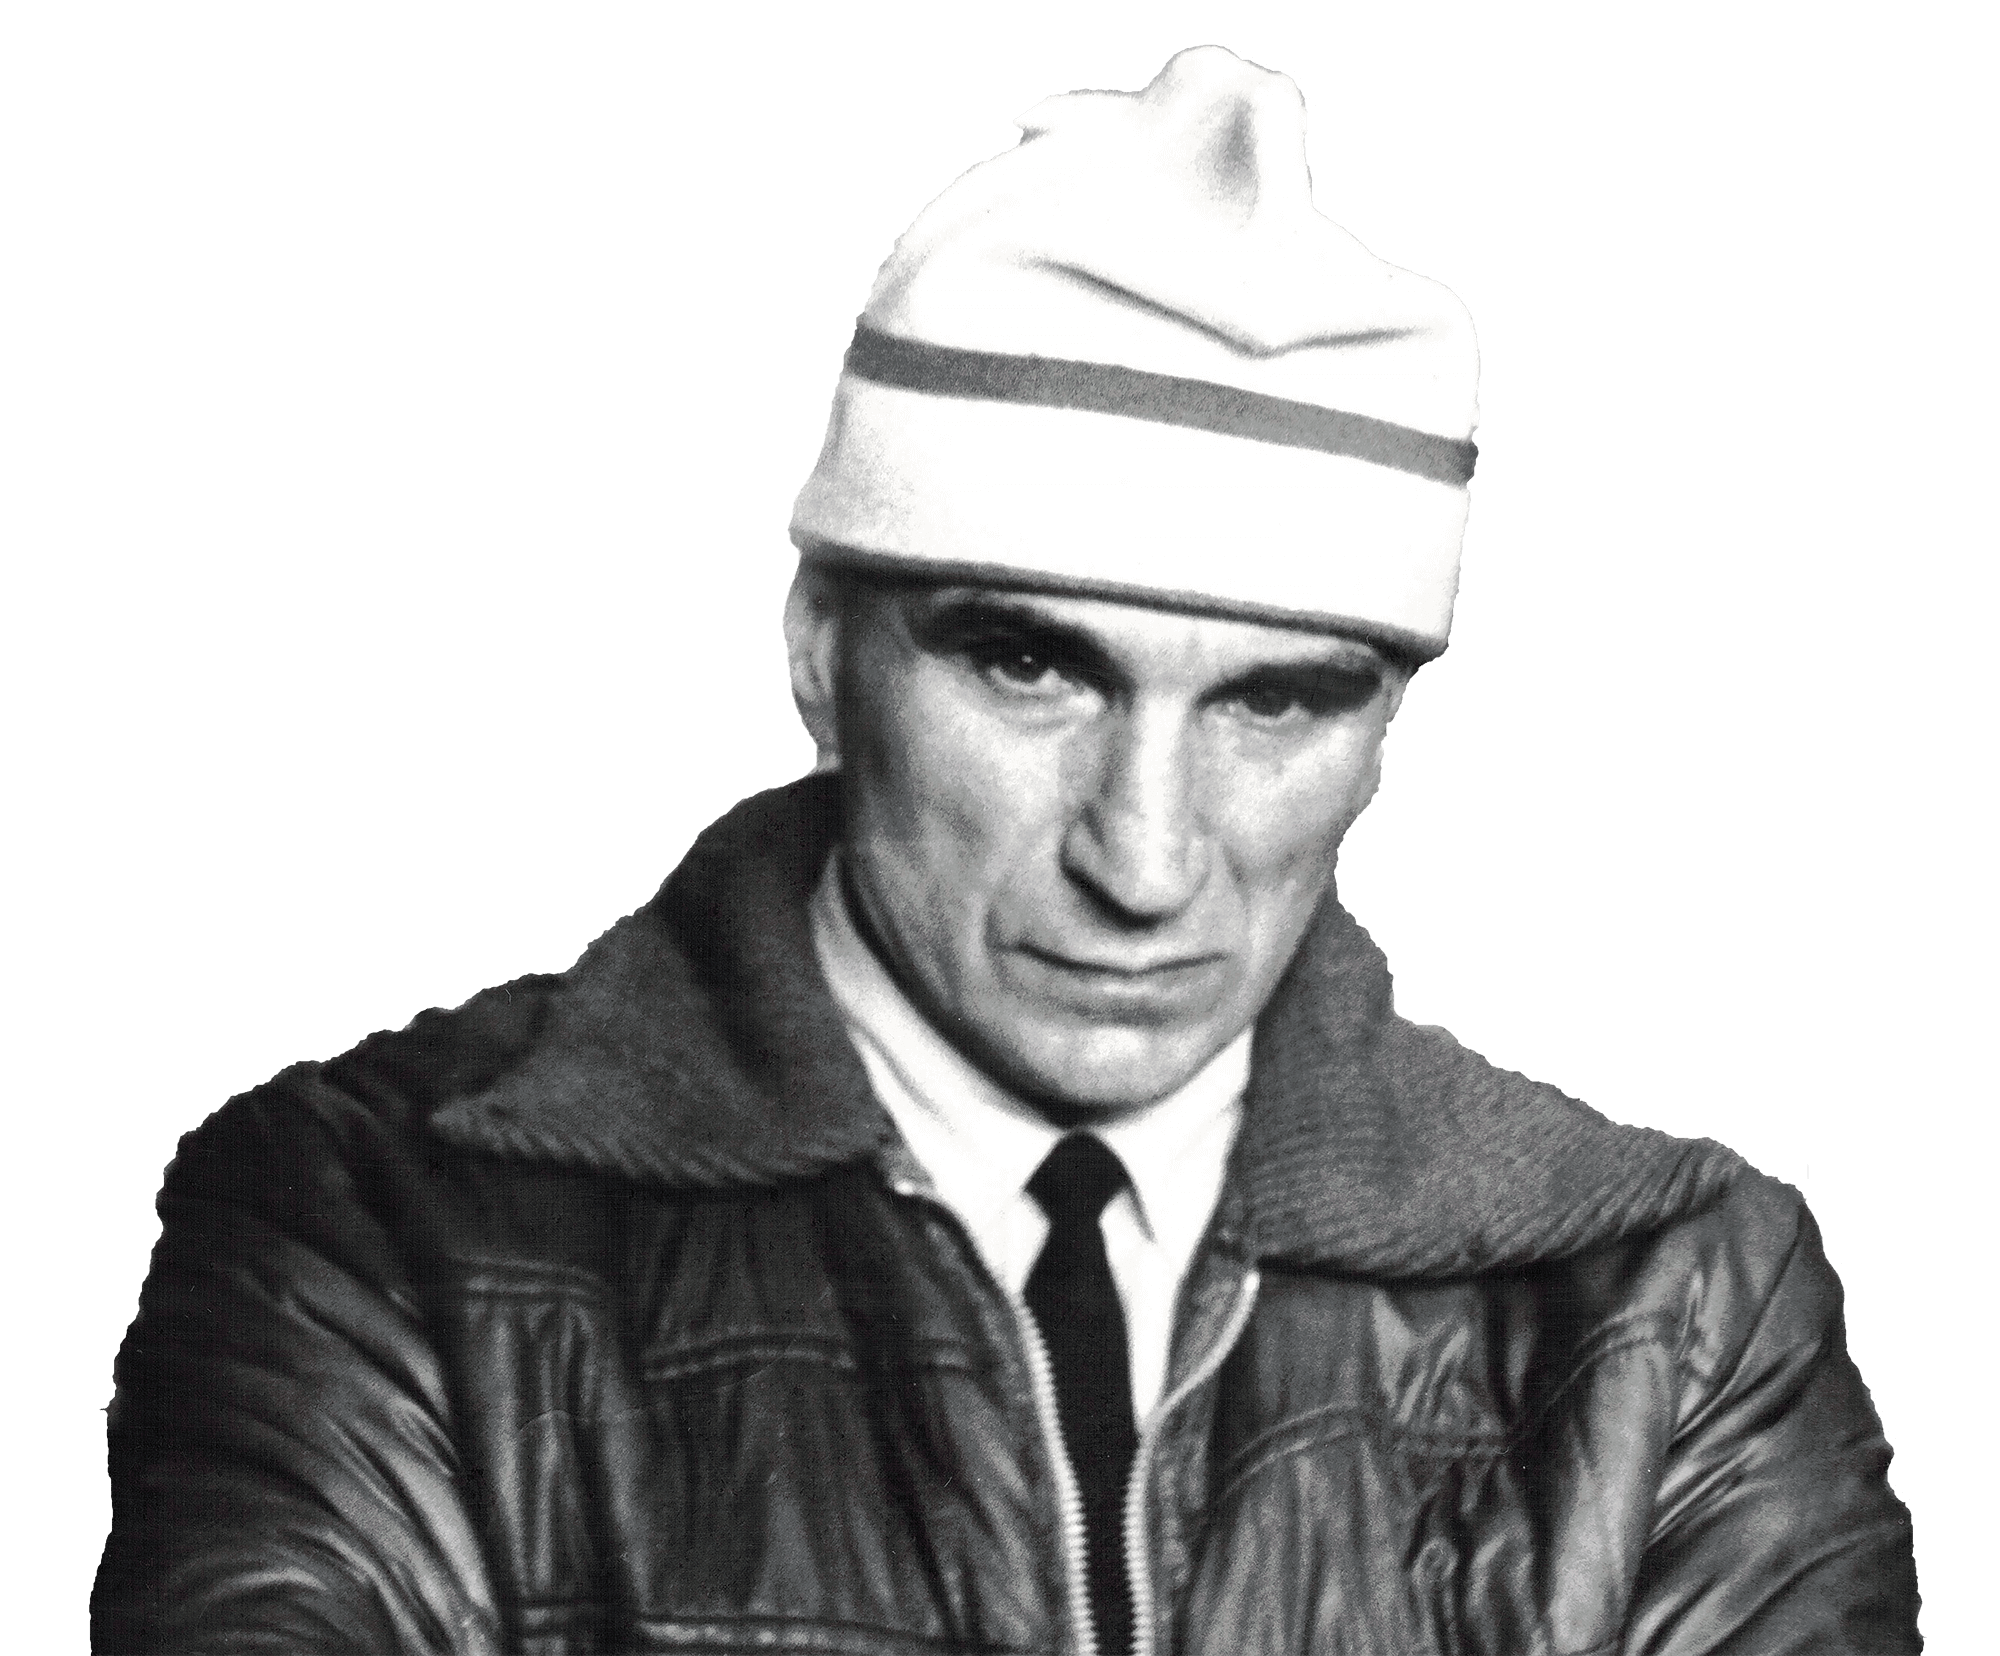
\includegraphics[width=3.35in,scale=1]{img/more_tough_gpa.png}}}
\AddToShipoutPicture*{\hspace{0cm}\put(20,220){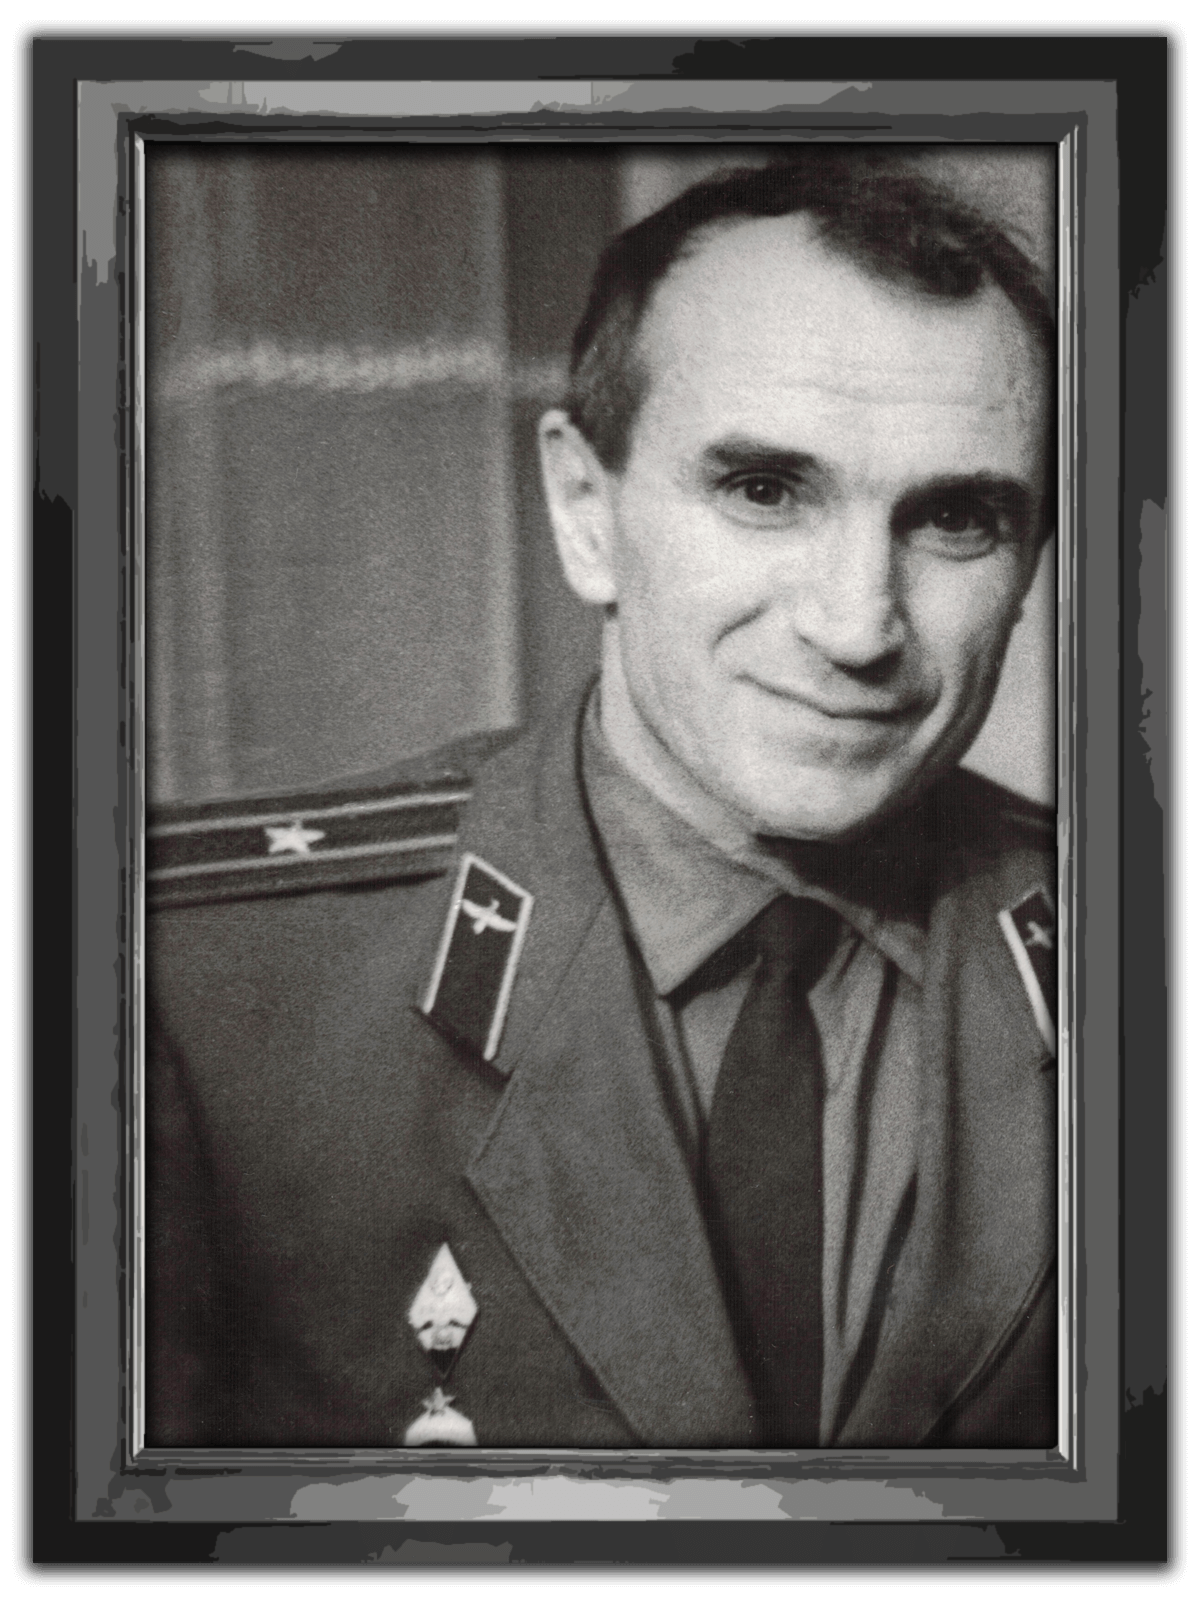
\includegraphics[width=2.2in,scale=1]{img/happy_army_small.png}}}
\AddToShipoutPicture*{\hspace{0cm}\put(30,440){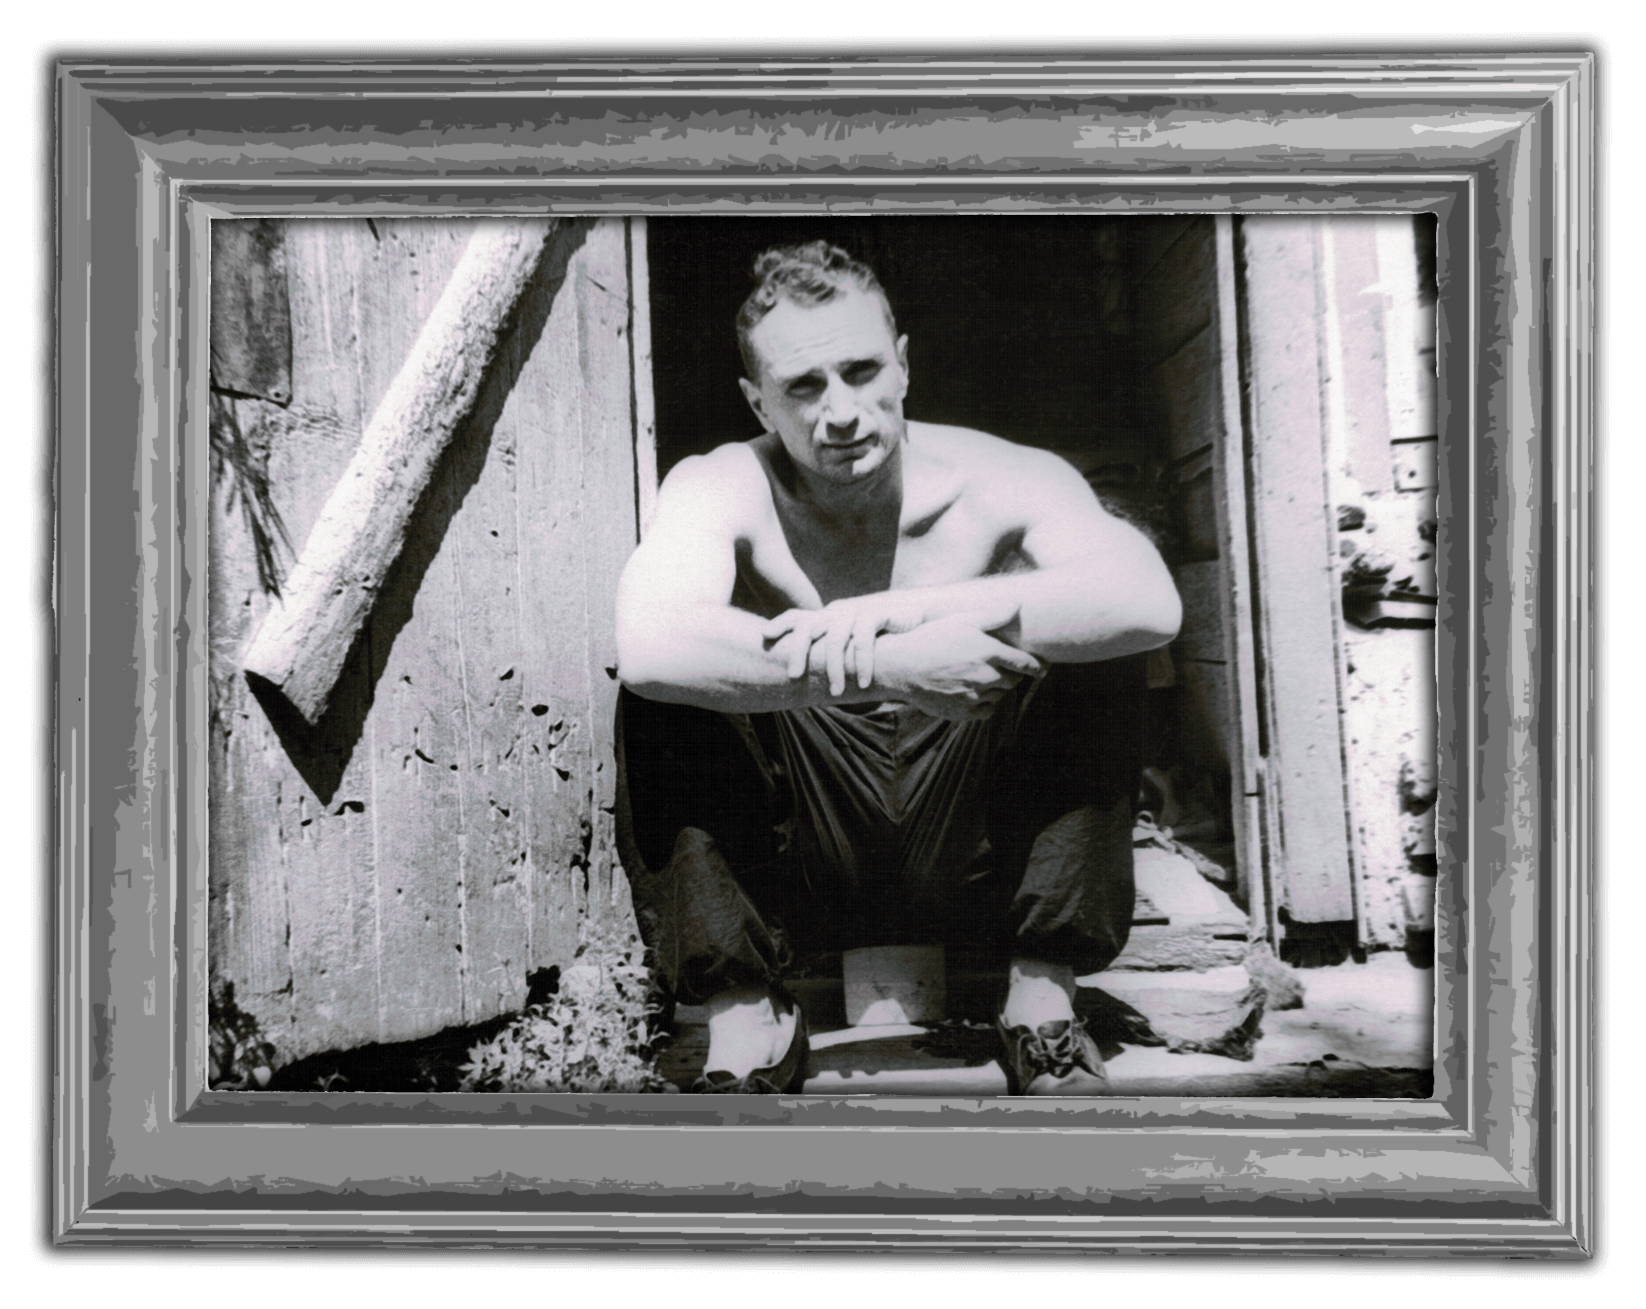
\includegraphics[width=2.5in,scale=1]{img/stoop_kid_frame.png}}}
\AddToShipoutPicture*{\hspace{0cm}\put(20,590){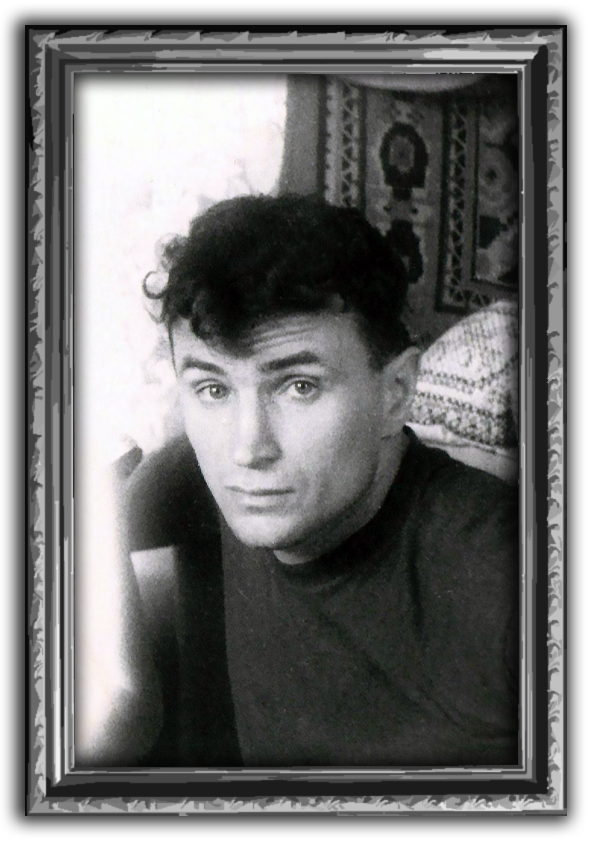
\includegraphics[width=1.8in,scale=1]{img/bedroom_eyes_frame.png}}}
But I digress. Taking as given the above, in order to ensure the future continues to be patterned in the image of Bymba’s will, it becomes necessary to more exactly clarify the nature of his preferences. Many of them could not help but be frustrated from the outset, and barring some paradigm shifting revolution in modern physics, will regrettably continue to be frustrated.  We could not and now cannot, for example, return him to the vigor and strength of his youth, though in some way its inverse – to not be trapped in a slow, ungainly body – has been satisfied. 
\\\\
Understanding what drives an individual – even one of quite intimate acquaintance – is no easy task. But we may hope to glean the exact structure of their preferences through the worlds they themselves strove to create or destroy. If they claim to prefer one world to another but in action are neutral between them, or else work in opposition to their claims, then their wills are not the same as those professed. This is, however, entangled with their power over the world – we would not say it is the revealed preference of the poor to starve when they do, nor ascribe great passion to the rich who’ve but to flex their fingers and satisfy every whim. Thus, it is also necessary to calibrate revealed preferences according to the degree of power wielded. But as mentioned, and as revealed through both his thoughts and deeds, many of Bymba’s preferences extended outside himself: he’d exhort me to stargaze at ungodly hours, to love and protect our wives and his daughters and fellow moral patients [paraphrasing], to read books and watch only the finest of Russian cinema produced between the years 1950 and 1990, to immanentize post-scarcity luxury space-communist utopia, to strike hard and fast and without mercy (yes) when the need to defend myself or others arises, to learn to tack a sailboat and recall the names of local plants and mushrooms, to kindly refrain from injuring myself while partaking in exercise, to engage in productive otium, to play the guitar and sing sea shanties in a loud baritone, to give all of myself not just to others but to myself as well, to alight from questionably tall structures into questionably deep bodies of water, and to walk upon the planet Mars. That last one, we’d meant to do together, with 2012 being our target date – sadly interrupted by a minor apocalypse. But a halved form of that day may yet come to pass, and several of the others should not be so difficult to bring about, either.
\\\\
I tried explaining some of these thoughts to Bymba once – his preferred form of immortality was rather more literal, and not in the Woody Allen sense. He instead aspired to become a sapient ball of light that would travel the universe in the company of sexy Martian babes. Not exactly what I’d had in mind. But I was prevented from sharing the perspective and so was never able to explain it to him fully, though its rough immaturity may have left much to be desired. Even so, it’s unclear if he might have sympathized with it, or else felt even stronger revulsion at the lack of purely psychological continuity. Luckily, this hot take on (not quite informational) immortality may not require informed, consenting participants. Even if he did not identify as strongly with his preferences, it’s still his preferences that formed the target of my love. And while the whole edifice is rather shaky, I have found its contemplation to provide some shelter from otherwise debilitating storms of grief. Sure, to the extent that my grandpa’s preferences can ever be satisfied according to such a distributed network of cause-and-effect, ample inefficiencies and reductions arise. But so long as the world occupies states more counterfactually aligned with grandpa’s will, the essence of his identity remains. So while I’m not able to reshape flesh and mind and return him to the living, I can help to protect that essence as best I can. 
\\

\AddToShipoutPicture*{\put(400,0){\includegraphics[width=3in,scale=1]{img/3boys_1army.png}}}
\AddToShipoutPicture*{\put(365,500){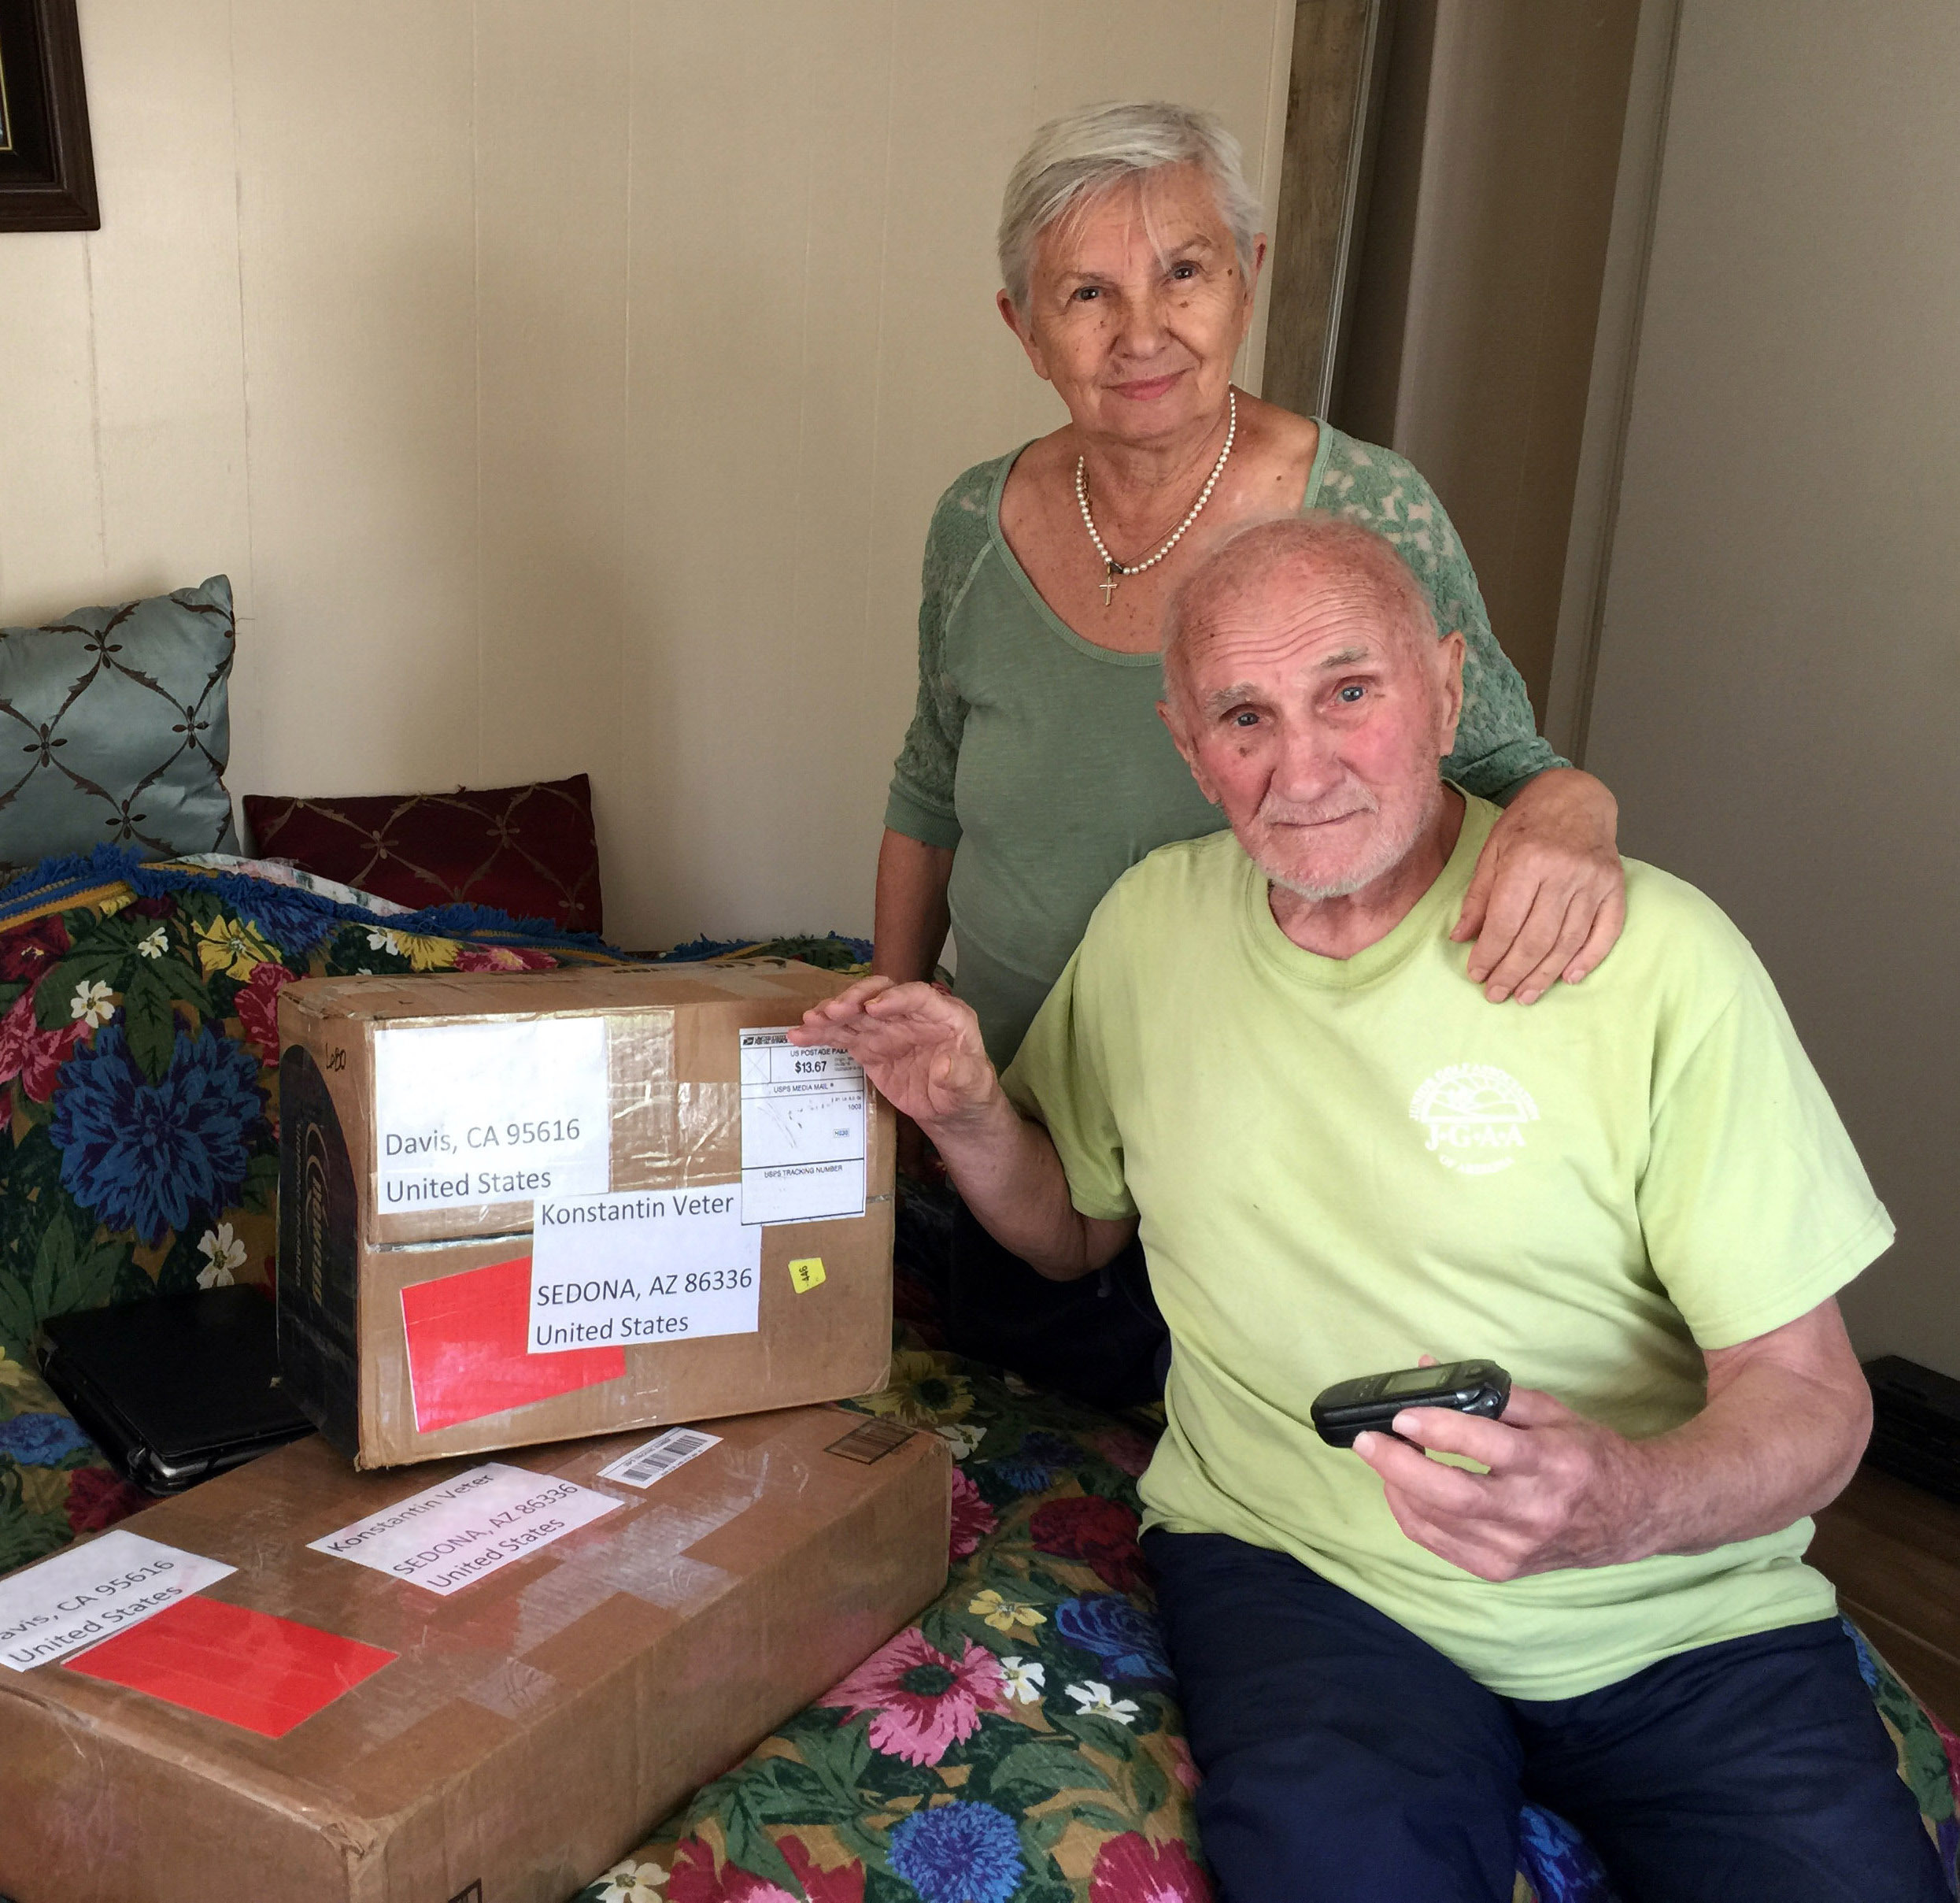
\includegraphics[width=3.25in,scale=1]{img/gpa_books.jpg}}}
\AddToShipoutPicture*{\put(453,490){\textcolor{DarkBlue}{\textit{Daunted by the latest book delivery.}}}}
\AddToShipoutPicture*{\put(400,180){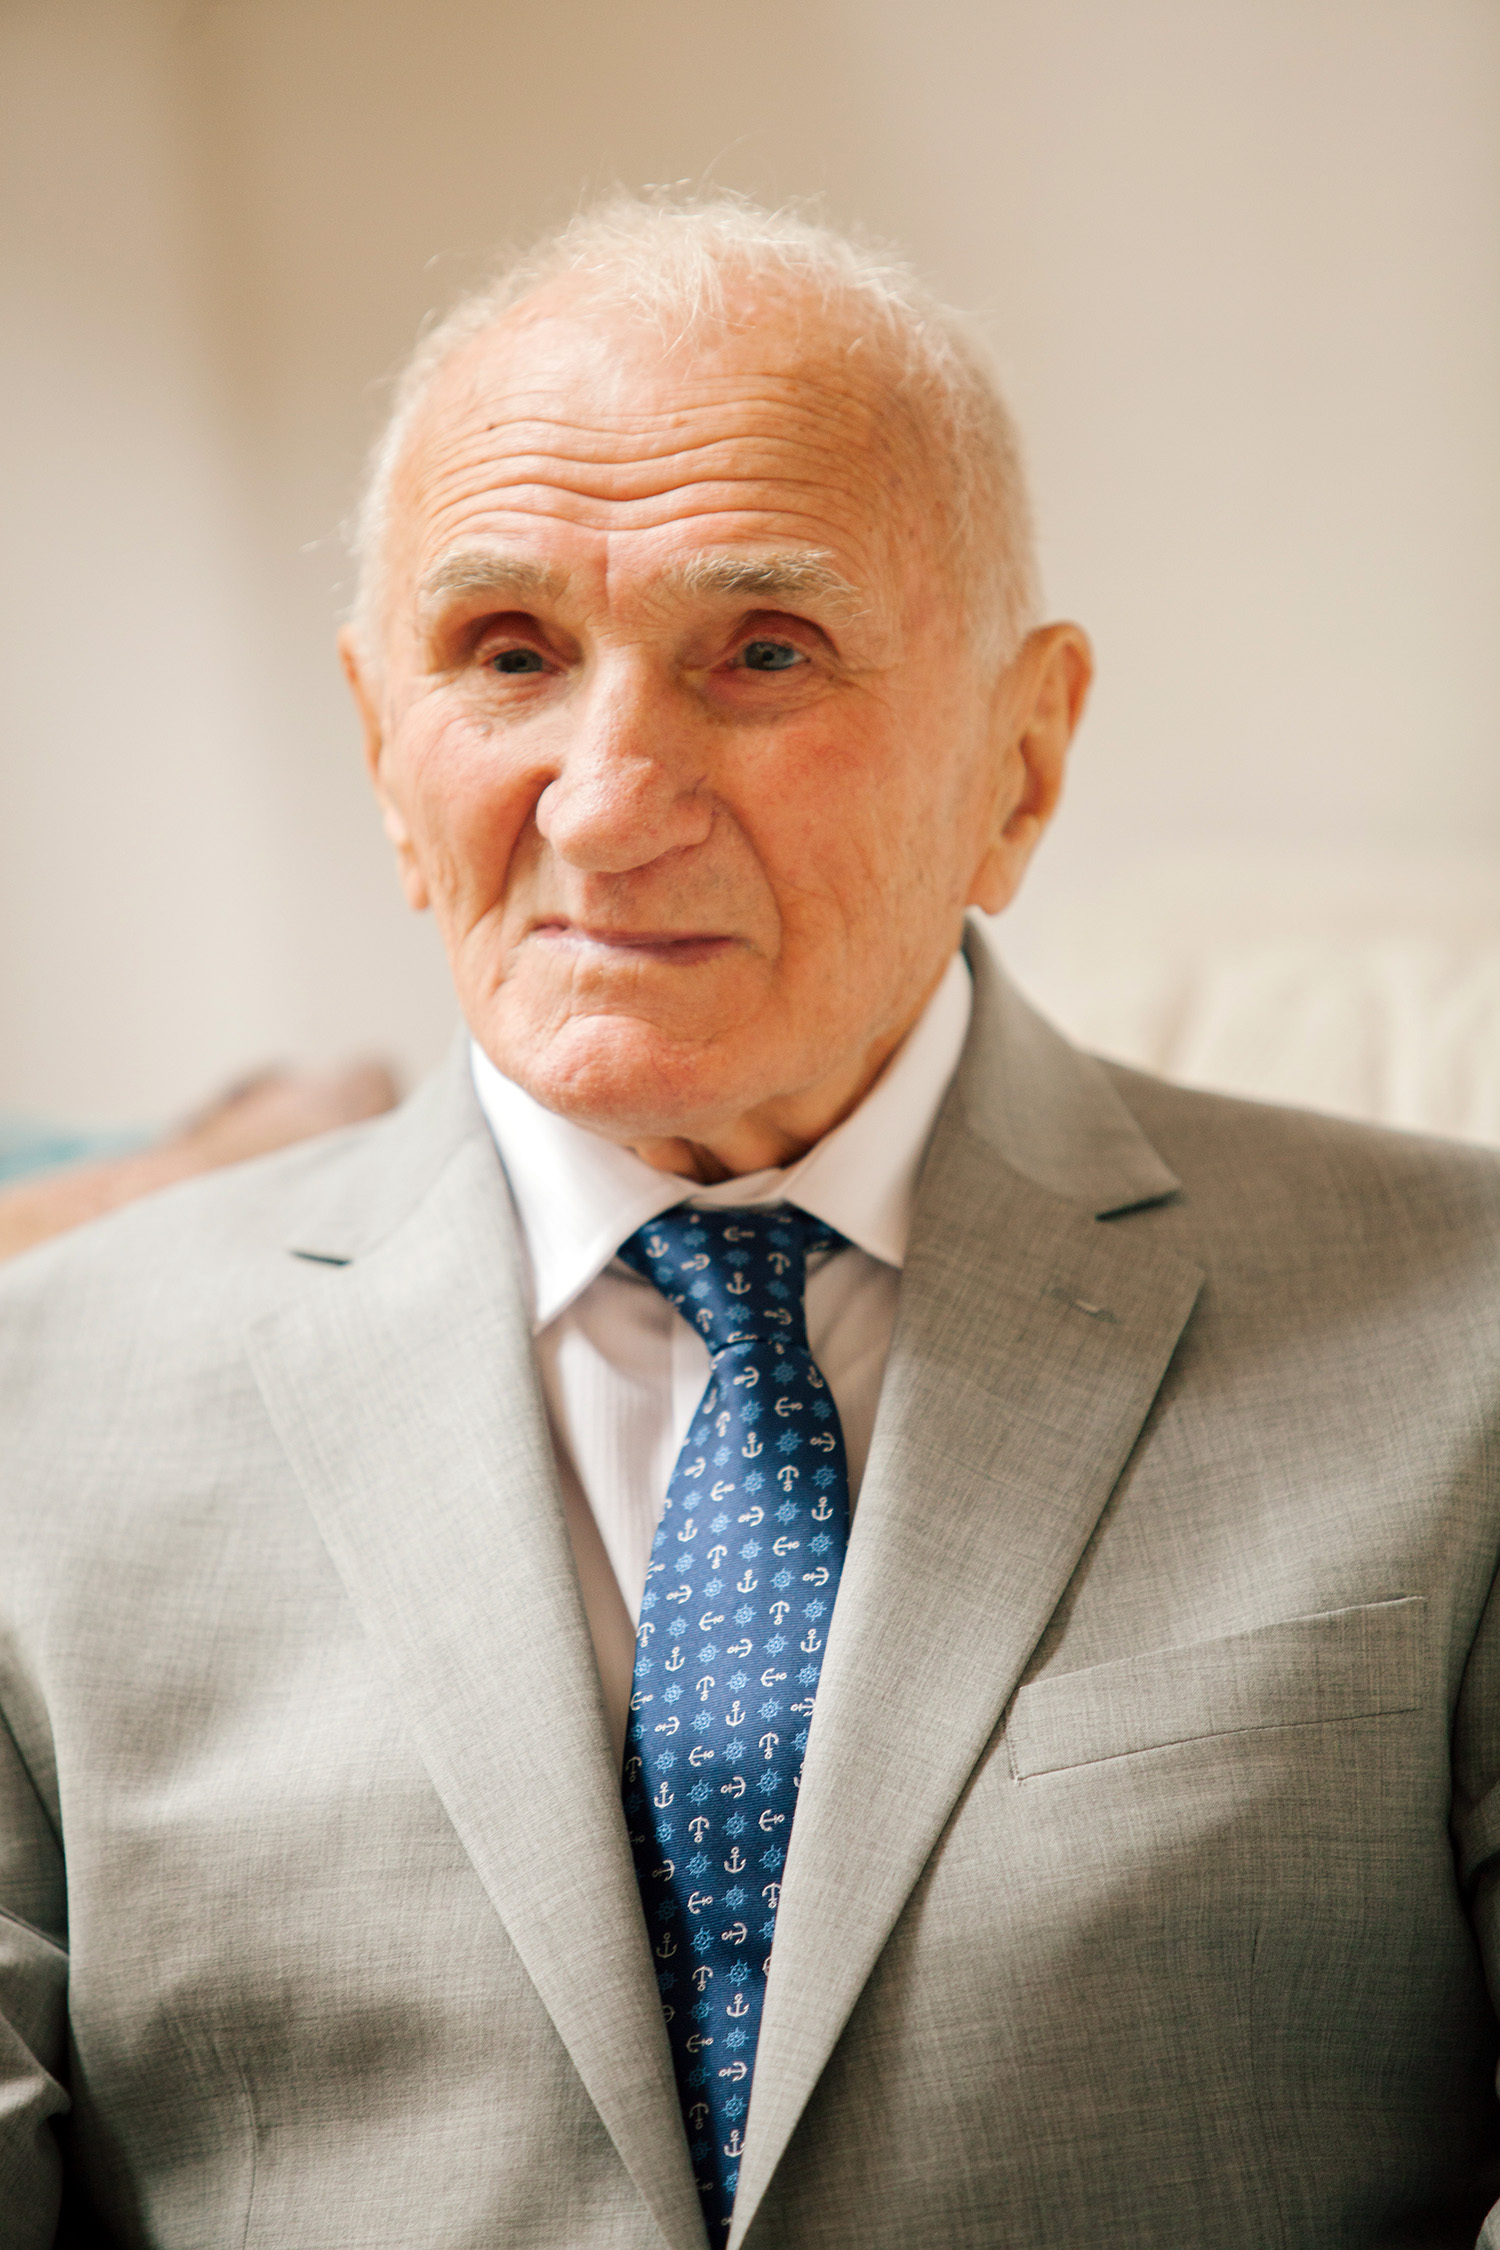
\includegraphics[width=2.75in,scale=1]{img/in_a_suit.jpg}}}
\AddToShipoutPicture*{\put(510,170){\textcolor{DarkBlue}{\textit{Persuaded into a suit.}}}}
\AddToShipoutPicture*{\put(290,51.5){
\includegraphics[width=1.5in, height=8.8in,scale=1]{img/white.png}}}
This framework also admits the possibility of healing ritual. Bymba did not desire cremation, and so instead of ash I procured a lock of his hair, thin and scraggly as it had grown during his final decades of life. By depositing individual strands at locations he’d longed to visit with me – the world’s oceans, the Black, Caspian, and Mediterranean seas, unspecified Martian trenches – I can strengthen the symbolic linkage between my own actions and Bymba’s will. I hope it proves cathartic.
\\\\
With respect to other would-be nepenthes: I’ve been offered many metaphors in the short time since Bymba’s death. These have often been grounded in mind-body dualism and invoked imagery of ships sailing into sunsets or birds taking flight to explore lands unknown. To me they’ve provided the opposite of comfort. But if I may be permitted my own metaphor, drawing upon the above-described framework in combination with my own proclivities and interests: imagine a distributed computing system, perhaps physically co-located in some dusty California server farm, with a head node assigning jobs across compute nodes. The latter are not otherwise idle, and indeed receive tasks from many other nodes – most of the time, it is in fact the head node contributing most of the relevant compute to its tasks, with other nodes providing spare resources only when able. These tasks may vary in their priority. Many can only be completed through interface with the head node, perhaps because they pertain to maintenance of head node hardware or because they involve specific head-node peripherals or operations only it can perform. But others are more general, and can be completed by any node in the network. Suddenly, total system failure fries the head node, fans spinning down and once cheerful status lights dimming as capacitors discharge. The head node is dead. It can no longer distribute new jobs. But the networked nodes yet live, and have in memory a long queue of unfinished tasks received from the now defunct head node. To the extent that a person is contained in their preferences, and exists insofar as those preferences are carried out, nonfunction of the head node does not require the cessation of all jobs received from it. And if a person only exists while those jobs are carried out, they may persist so long as those tasks remain active, saturating available compute, slowed in the global sense and critically compromised but not canceled outright. So long as loyal networked nodes survive, the work of the head node goes on.
\\

\AddToShipoutPicture*{\put(0,-10){
\includegraphics[width=3in,scale=1]{img/gpa_baby.png}}}
\AddToShipoutPicture*{\put(15,570){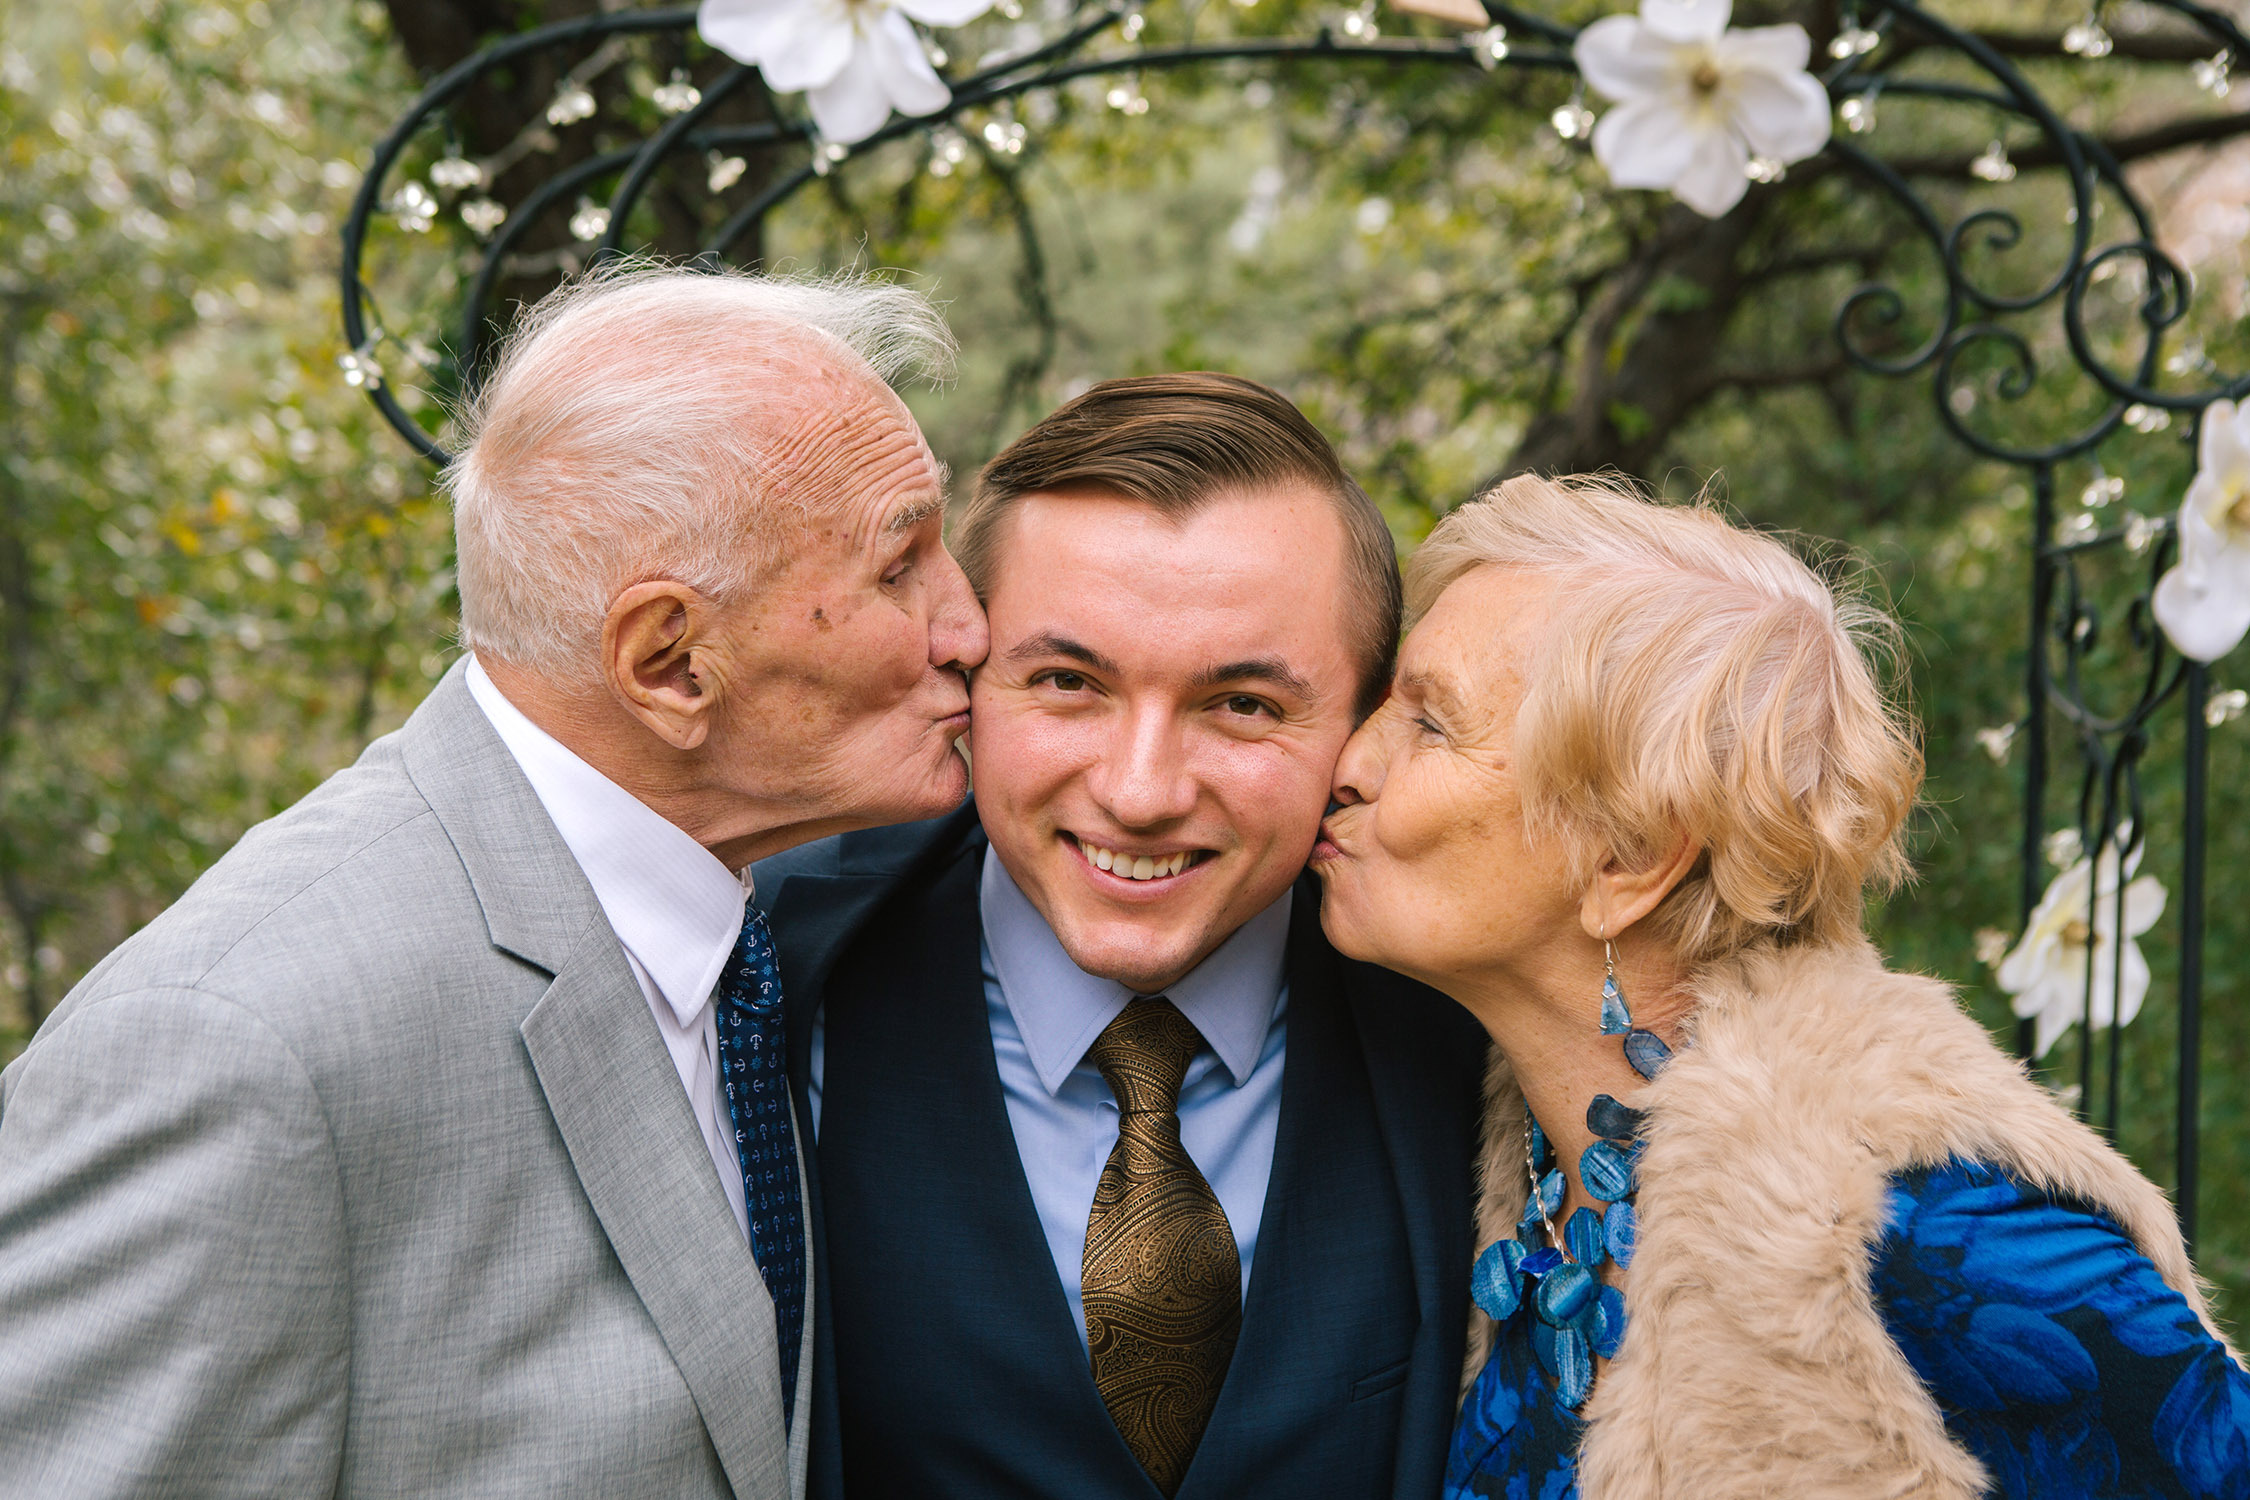
\includegraphics[width=3.25in,scale=1]{img/gparents_kiss.jpg}}}
\AddToShipoutPicture*{\put(15,400){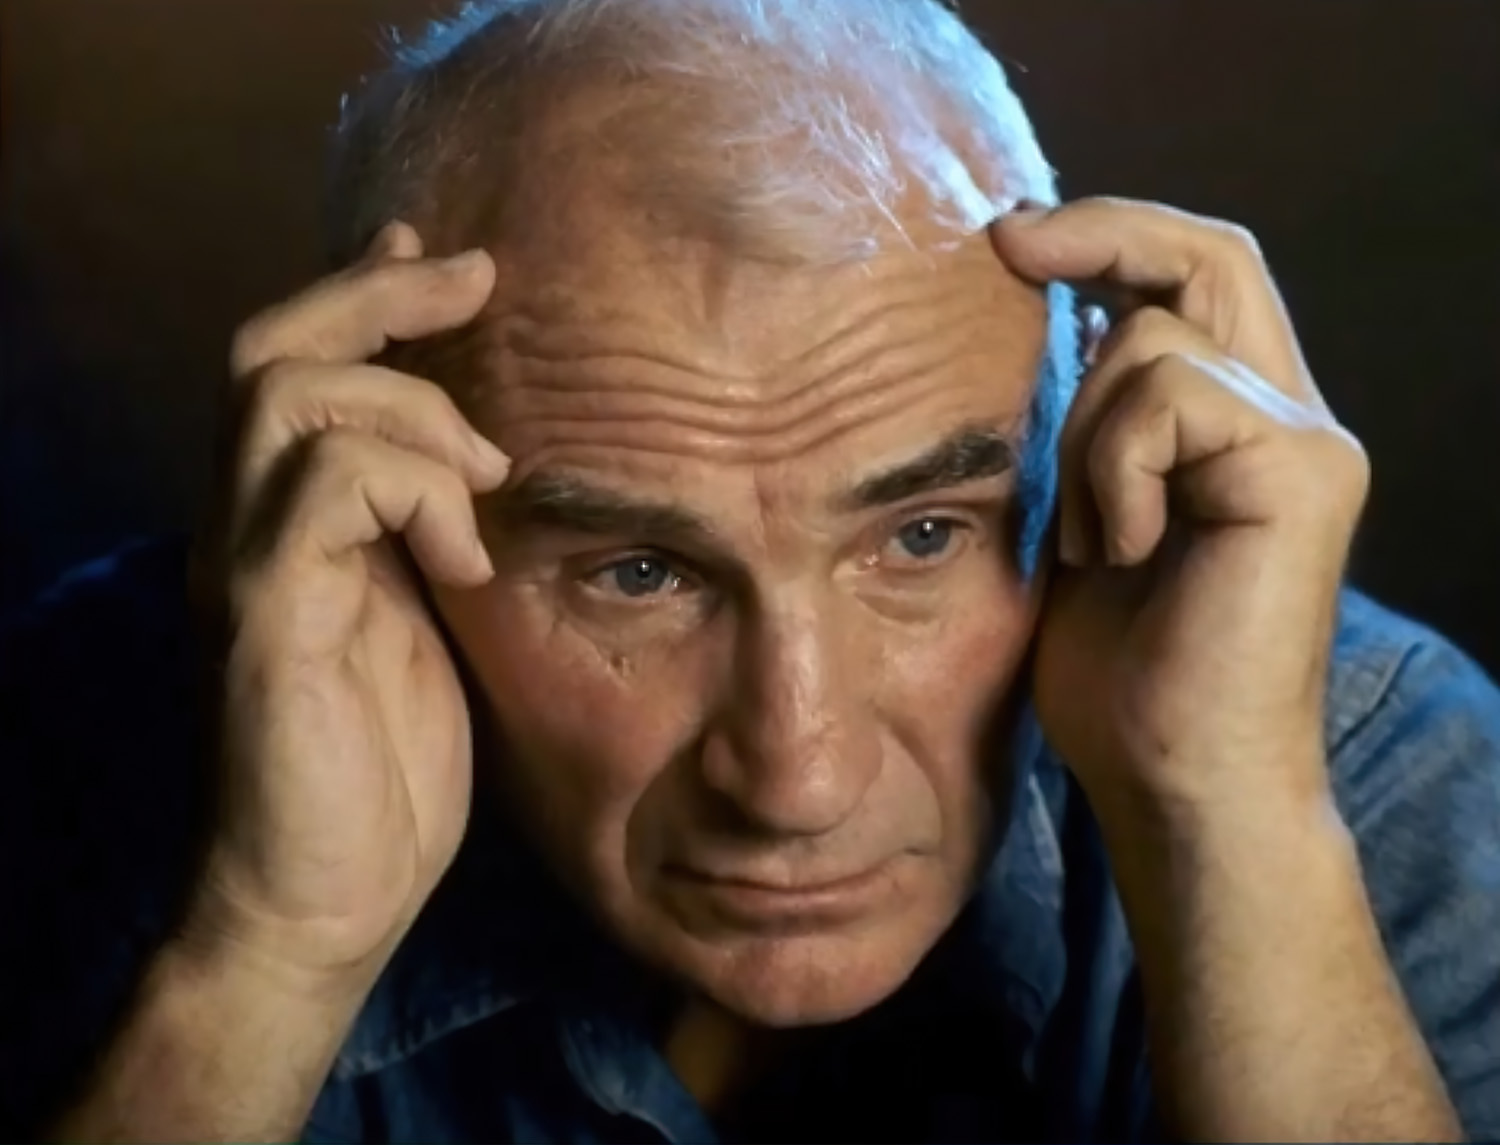
\includegraphics[width=2.75in,scale=1]{img/thoughtful_grandpa_2.jpg}}}
\AddToShipoutPicture*{\put(15,115){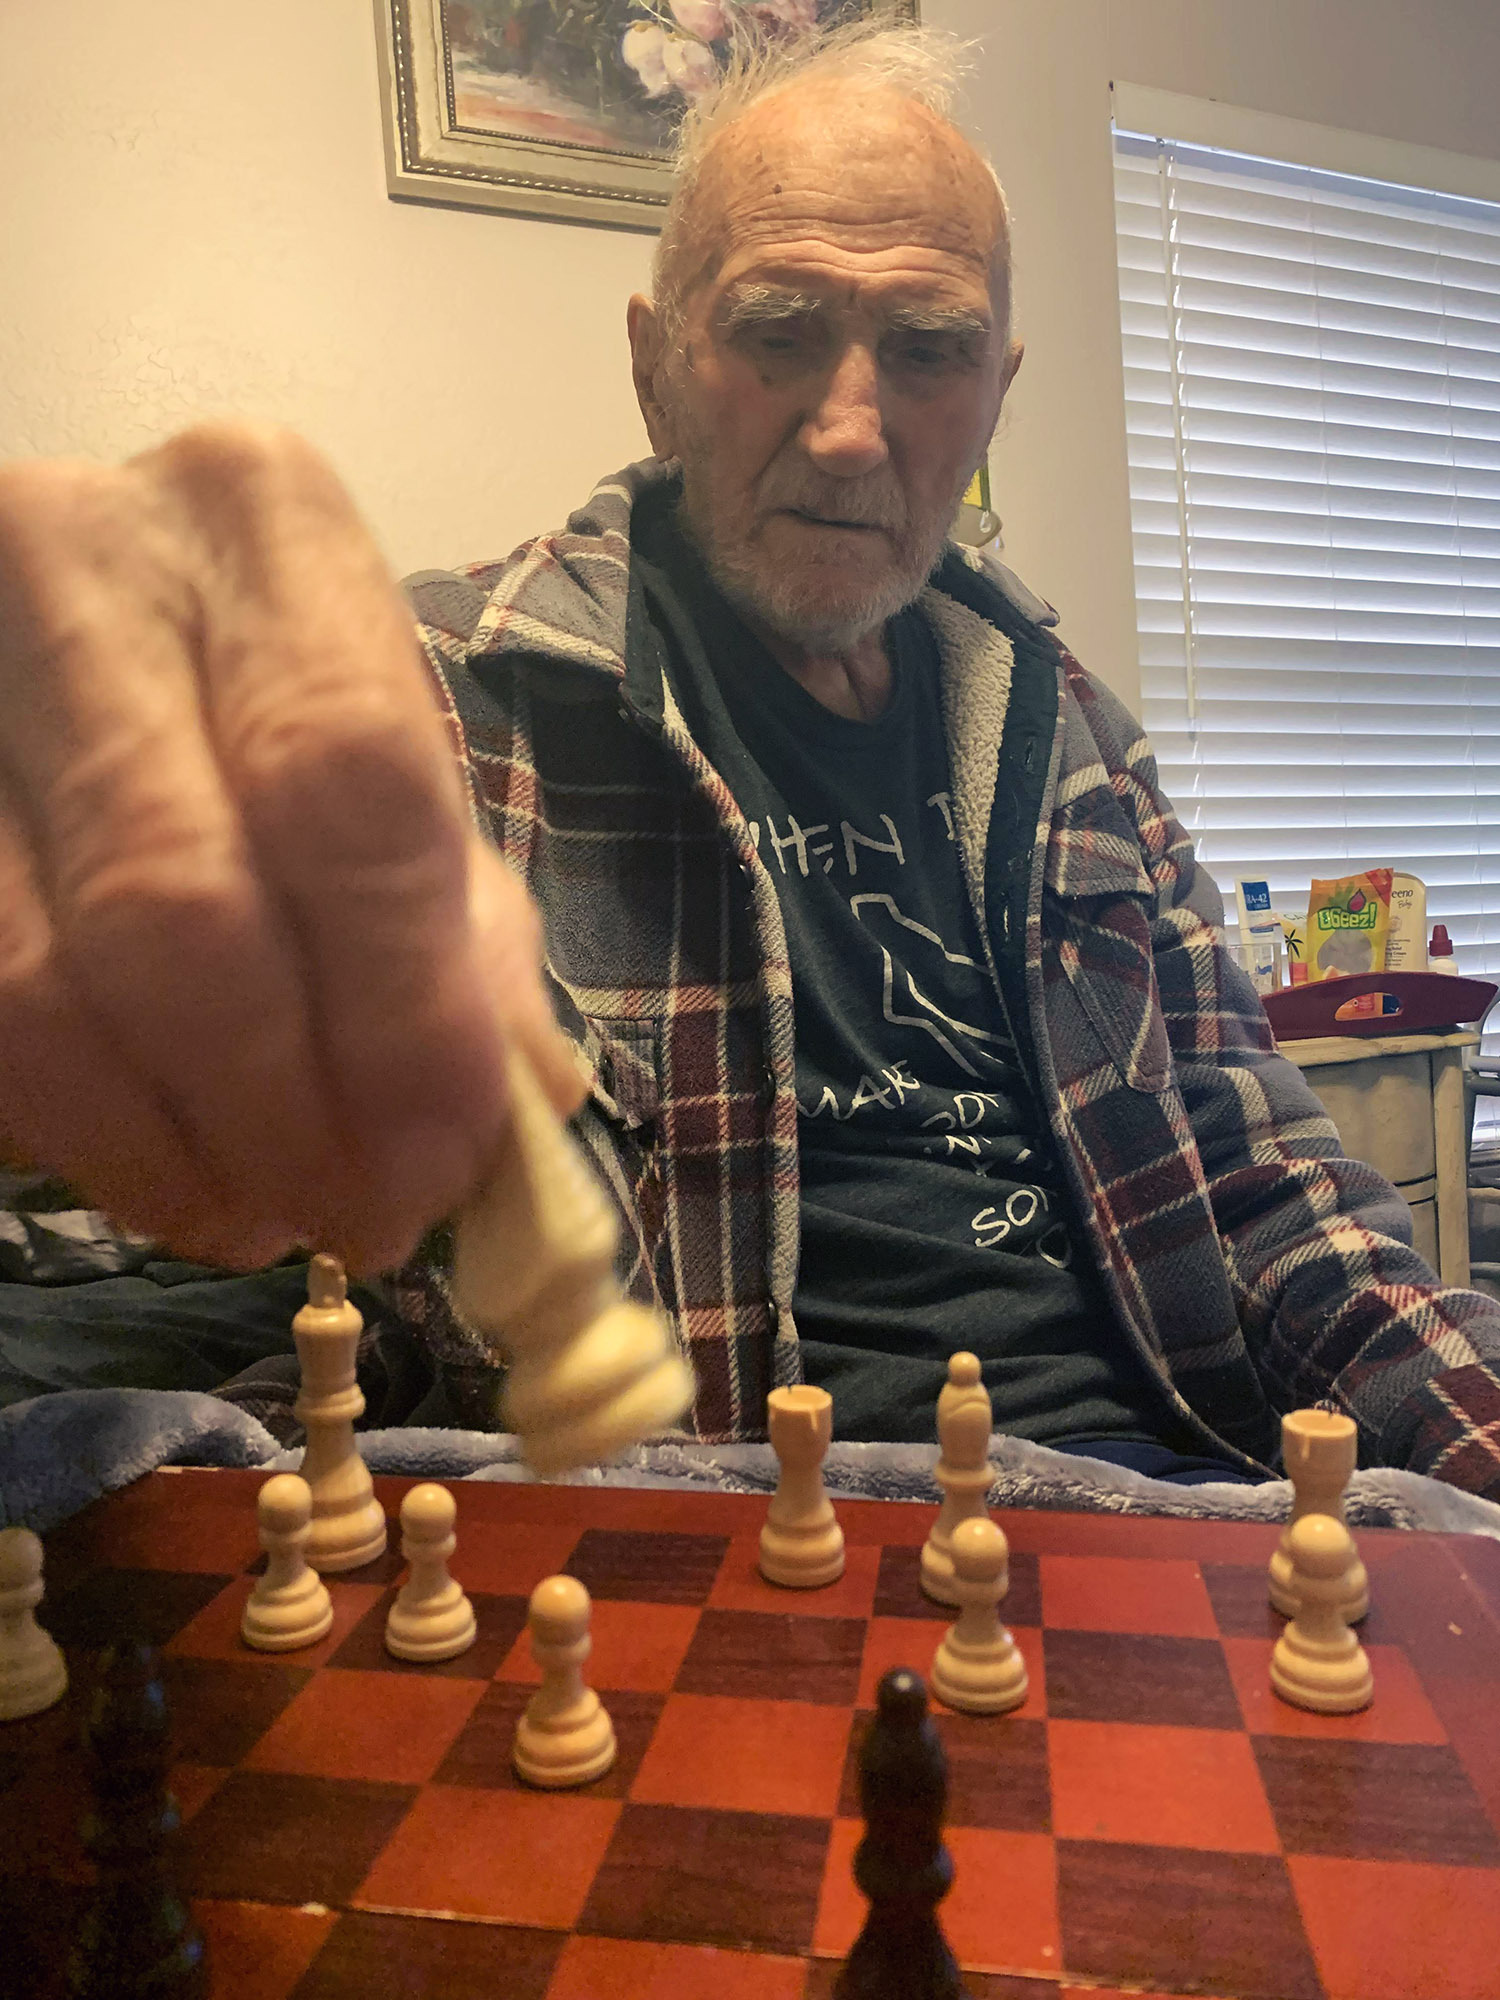
\includegraphics[width=2.75in,scale=1]{img/last_chess_small.jpg}}}
\AddToShipoutPicture*{\put(230,15){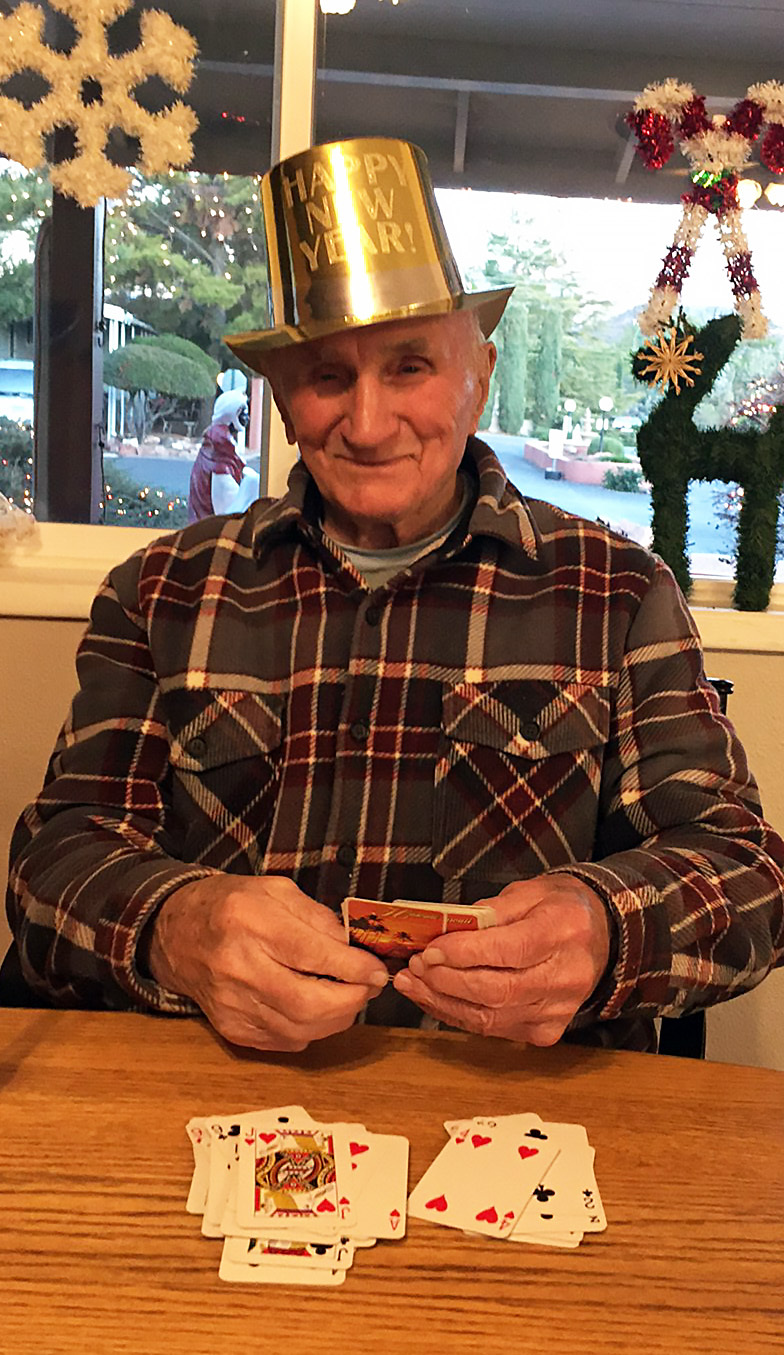
\includegraphics[width=2.5in,scale=1]{img/gpa_cards.jpg}}}
\AddToShipoutPicture*{\put(230,15){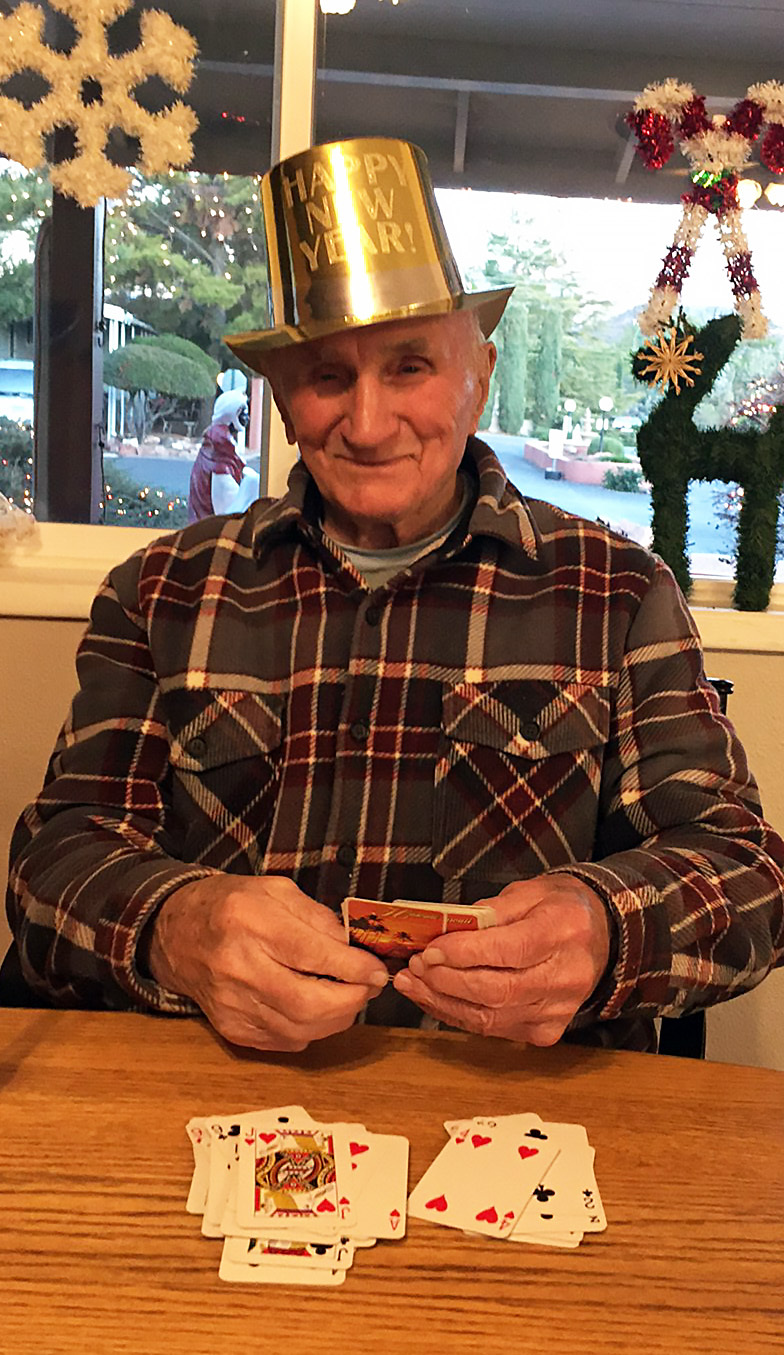
\includegraphics[width=2.5in,scale=1]{img/gpa_cards.jpg}}}
%\AddToShipoutPicture*{\put(427.5,15){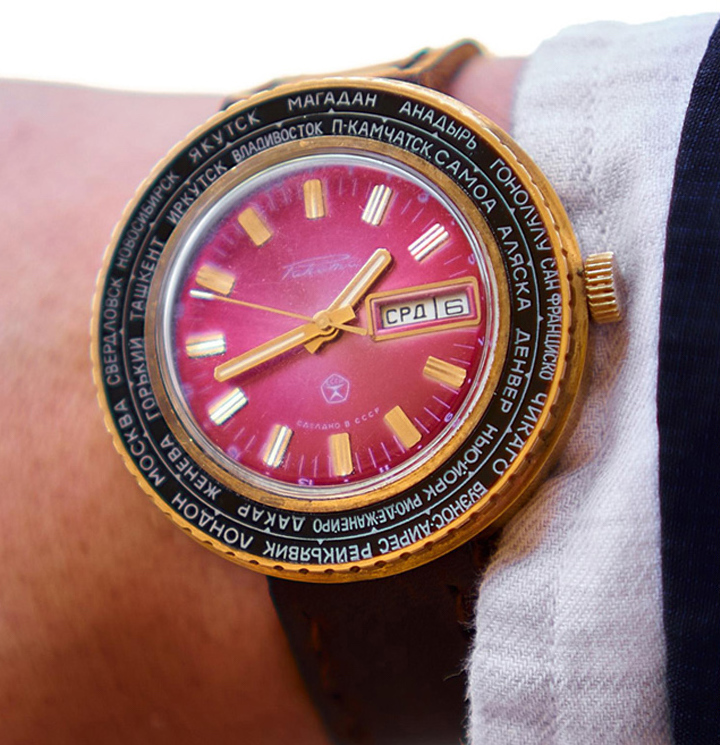
\includegraphics[width=2.35in,scale=1]{img/gpa_watch.jpg}}}
\AddToShipoutPicture*{\put(427.5,15){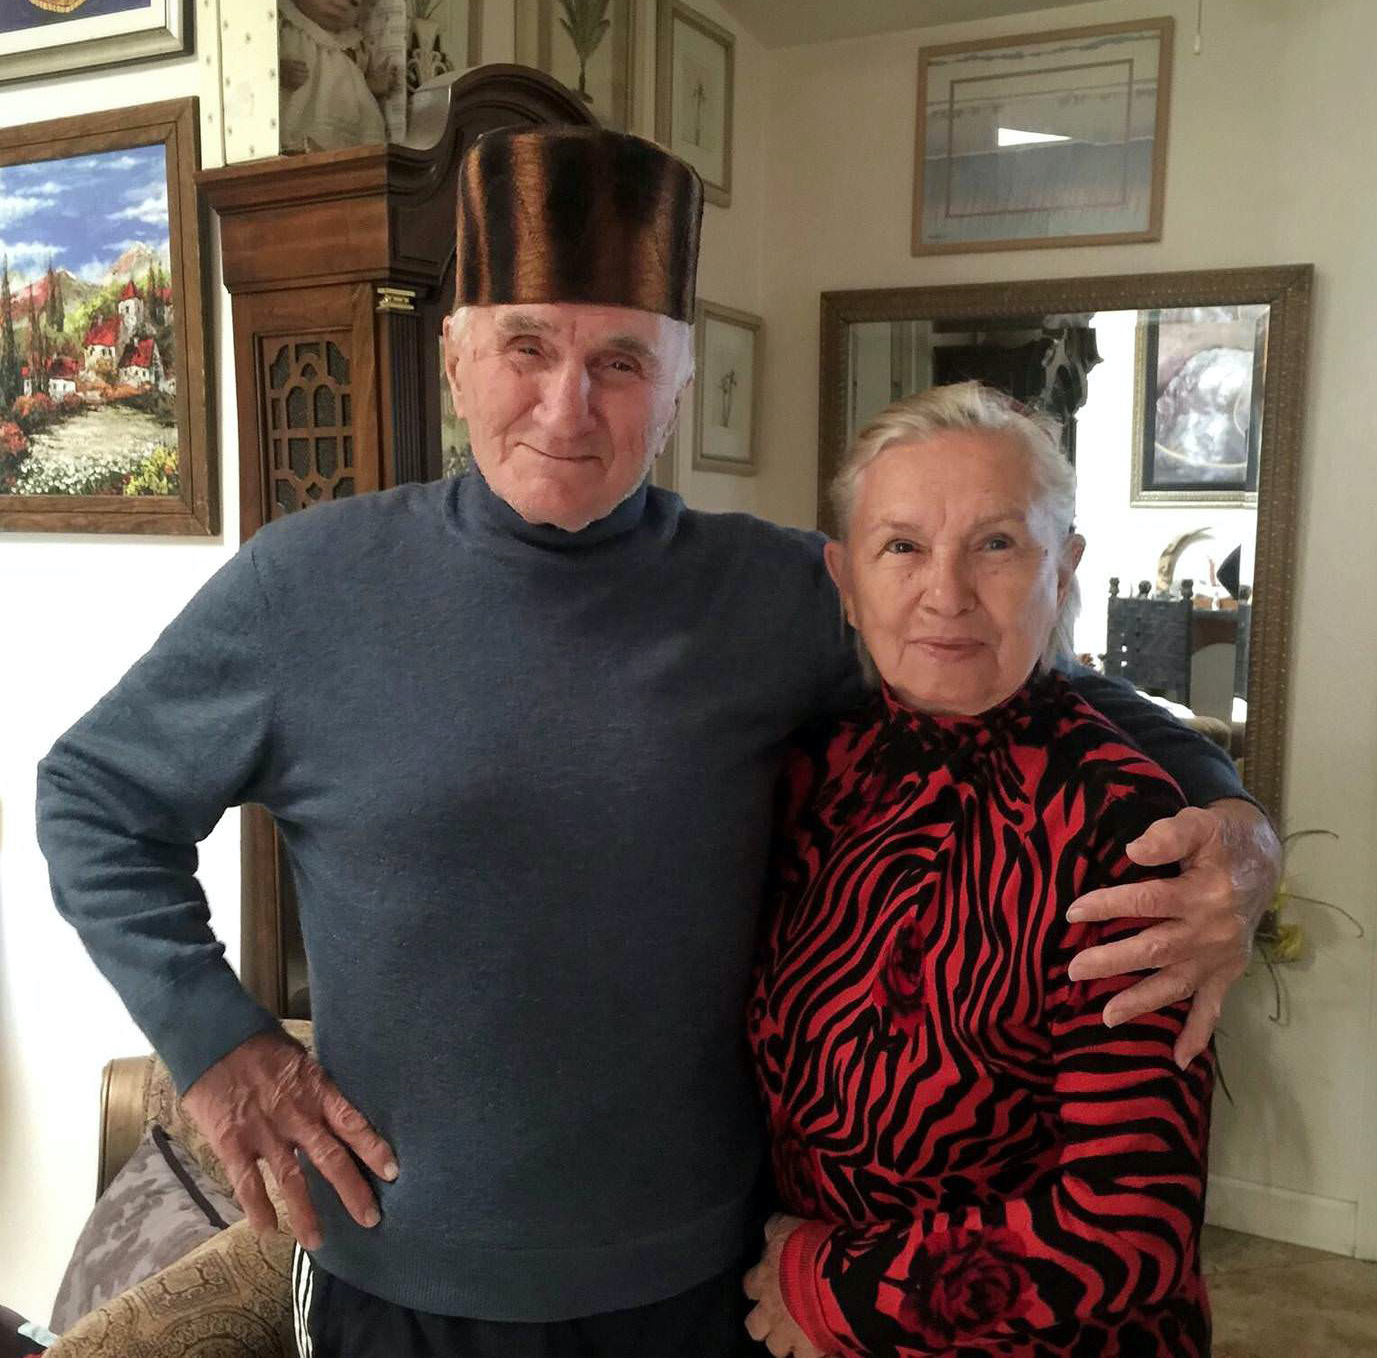
\includegraphics[width=2.35in,scale=1]{img/gma_gpa_young_2.jpg}}}
\AddToShipoutPicture*{\put(427.5,198){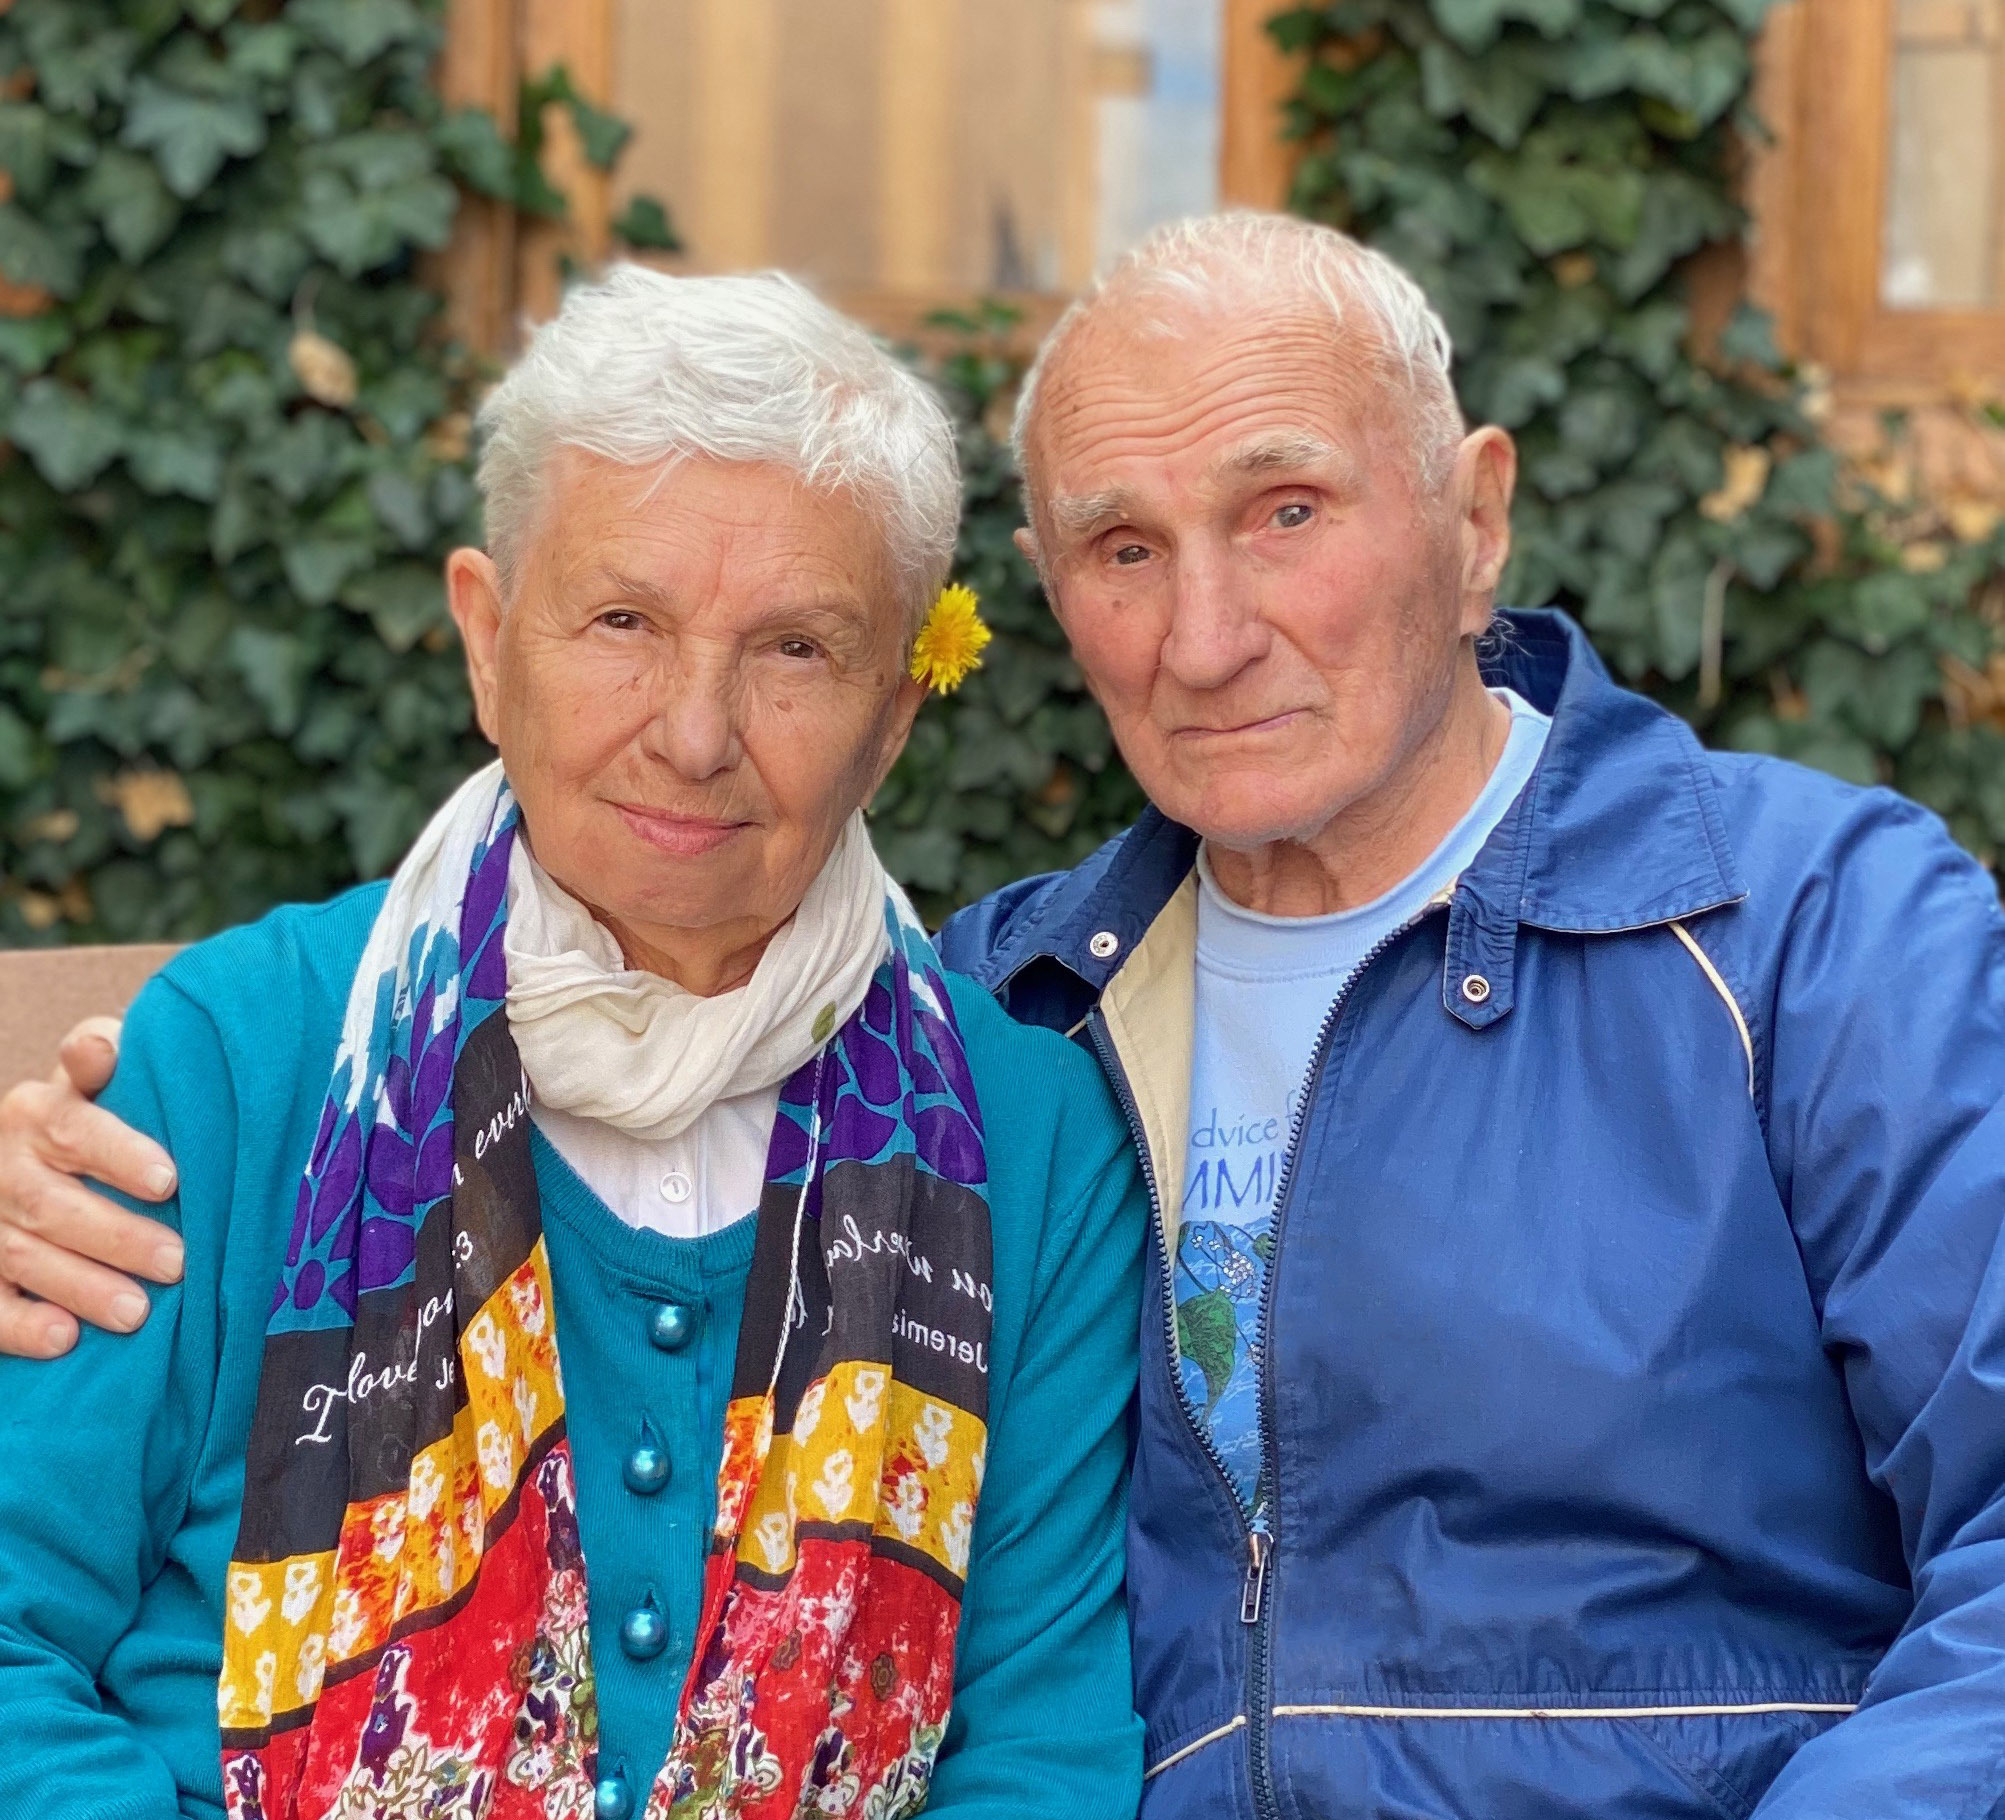
\includegraphics[width=2.35in,scale=1]{img/gparents_new_2.jpg}}}
\AddToShipoutPicture*{\put(215,329.5){
\includegraphics[width=2.25in, height=4.95in,scale=1]{img/white.png}}}

\end{article*}

\begin{article*}

\newgeometry{left=0.8in,right=0.8in,top=1in,bottom=1in}

\onecolumn
\invisiblesection{Poetry}
\vspace*{0.775in}
I don’t think Bymba was aware of death poems, most famously the \textit{jisei}: his was a pen built for prose and not poetry. So I – weeb that I am – will compose one in his stead. It won’t abide by any established metrical or thematic standards, out of respect for his disregard of the form.\\\\

\hspace*{\fill}\textbf{\Large What was once unyielding now yields}\\

\hspace*{\fill}Dreaming of shooting stars and deep waters \\
\hspace*{\fill}Of Martians and spaceships and rushing wind\\ 
\hspace*{\fill}Of family and laughter and friends\\
\hspace*{\fill}I fade from this world\\
\hspace*{\fill}My thoughts a haze, drifting over oceans of memories\\
\hspace*{\fill}Of starry villages and fractious daughters\\
\hspace*{\fill}Ringed in flowers and pine trees\\
\hspace*{\fill}With happy dogs, fur golden-red\\
\hspace*{\fill}Bounding through fields and into lakes, chasing sticks\\

\hspace*{\fill}On my lips the echo of youth and strength and potential\\
\hspace*{\fill}It tastes of bread and butter and borsch\\
\hspace*{\fill}Of saltwater, sweat, and salo\\
\hspace*{\fill}So much to do, so much to see! But no more.\\
\hspace*{\fill}My journey complete, I pass into memory\\
\hspace*{\fill}And leave behind many unfinished works\\
\hspace*{\fill}They will have to be finished without me\\

\hspace*{\fill}All that remain are farewells\\
\hspace*{\fill}Farewell, cruel age!\\
\hspace*{\fill}Farewell, withered stumbling body!\\
\hspace*{\fill}Farewell, infirmity and sickness.\\
\hspace*{\fill}I will miss many, but I will not miss you.\\

\hspace*{\fill}My old refrain,\\
\hspace*{\fill}To always remember, love, and wait\\
\hspace*{\fill}Perhaps one last time.\\

\hspace*{\fill}Goodbye.

\AddToShipoutPicture*{\hspace{0cm}\put(20,0){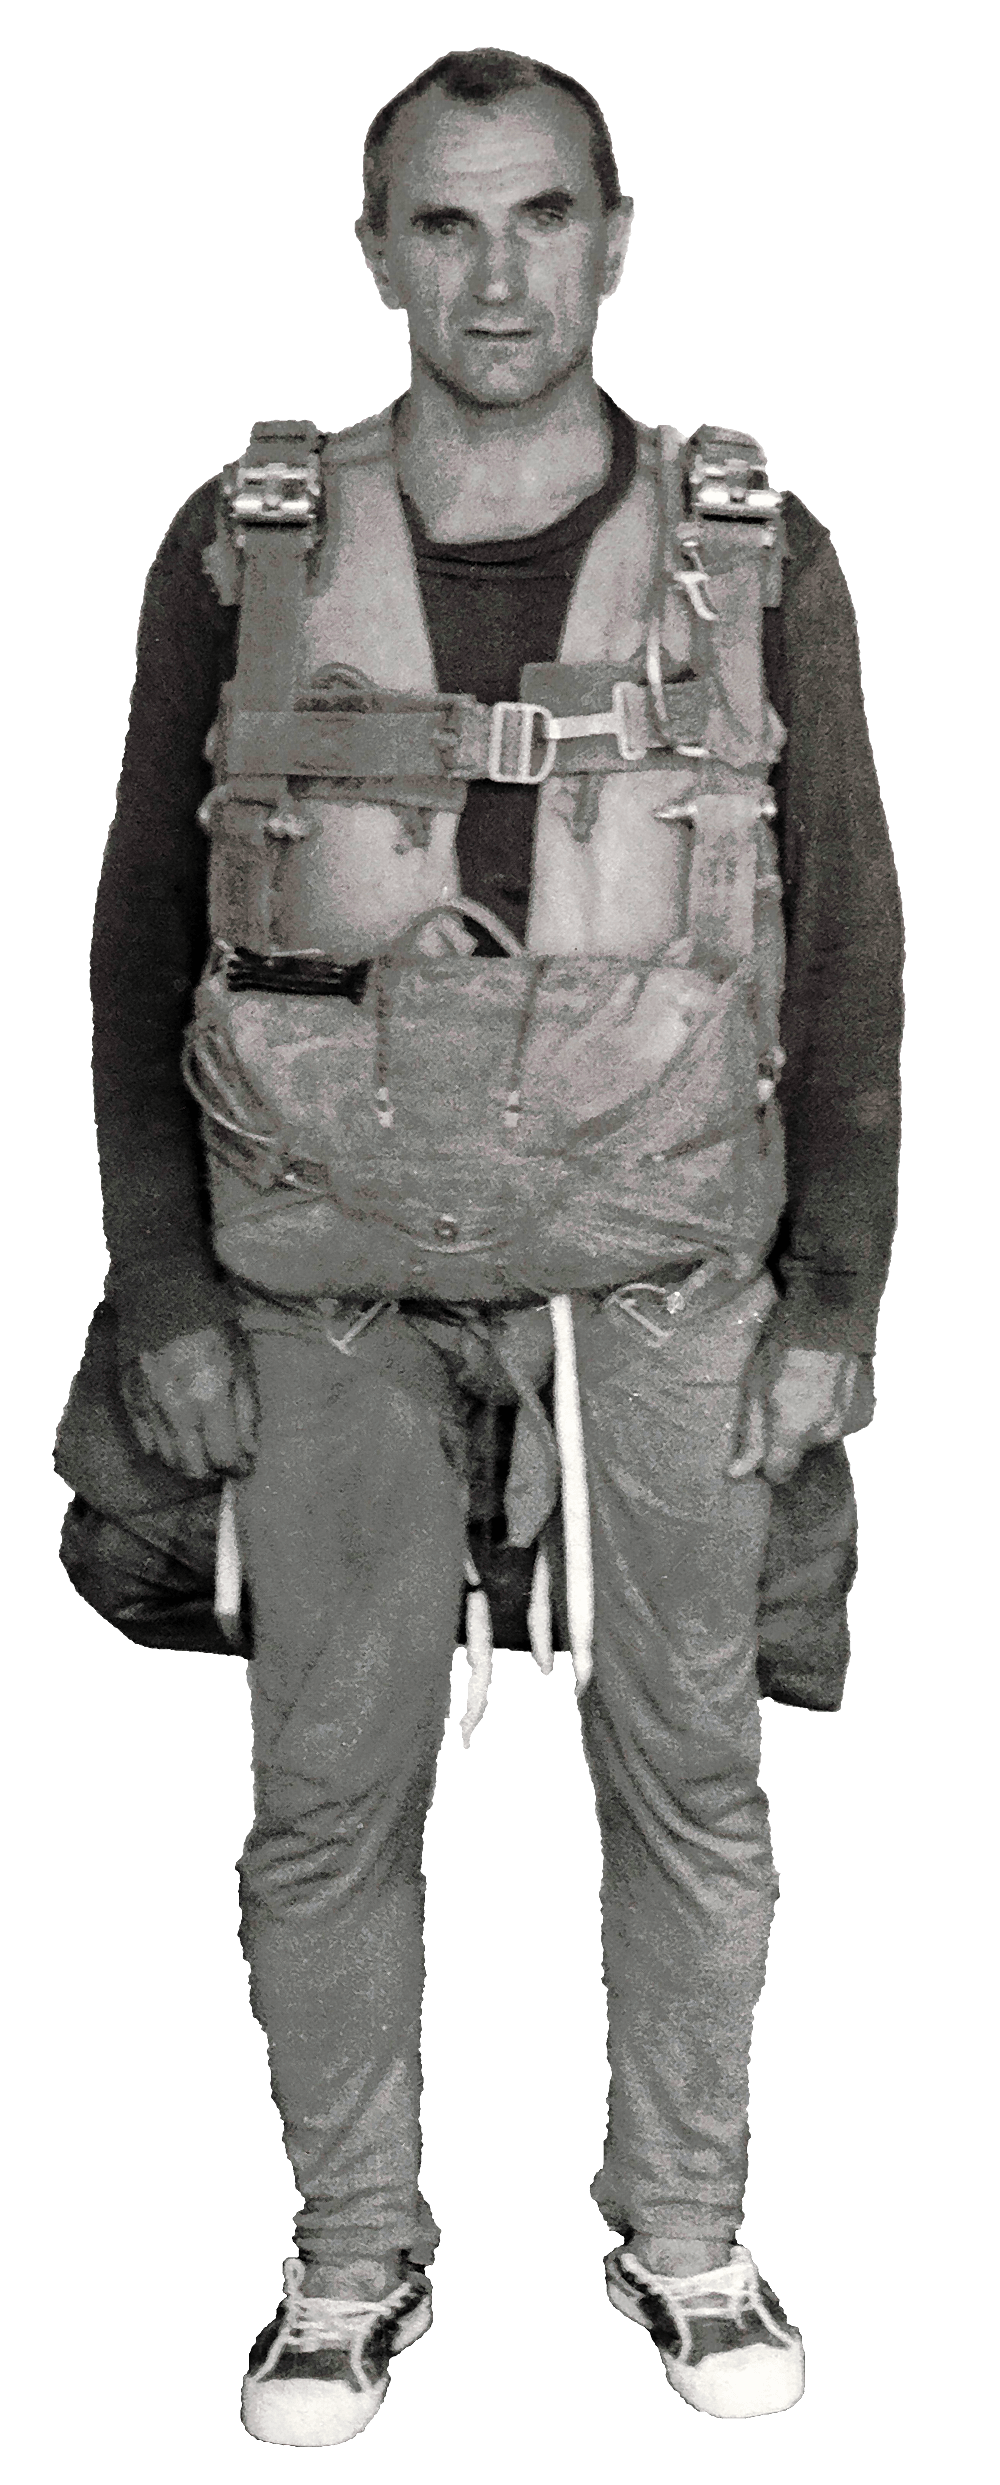
\includegraphics[width=2.05in,scale=1]{img/bymba-skydiver_evensmaller.png}}}
\AddToShipoutPicture*{\hspace{0cm}\put(20,370){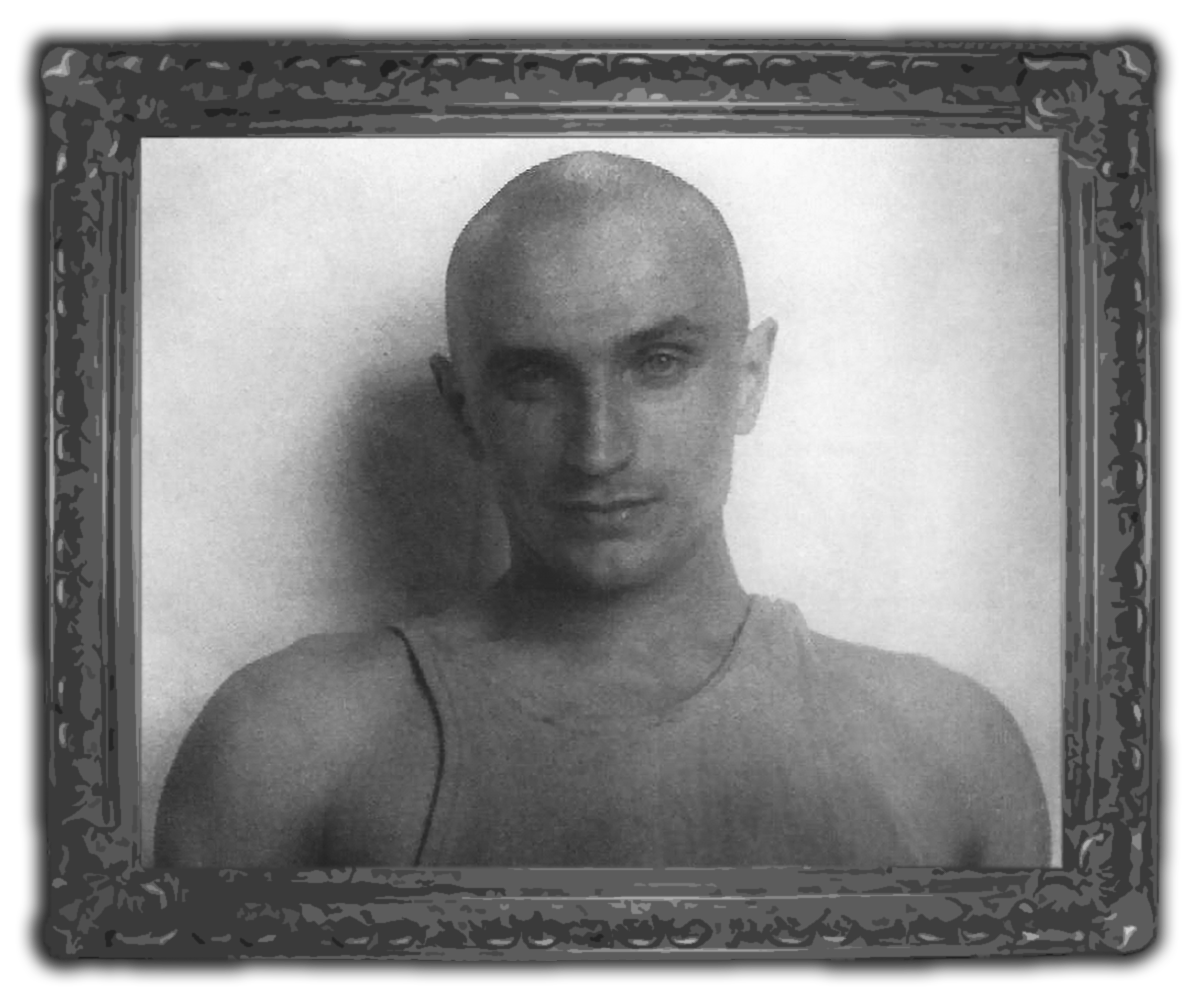
\includegraphics[width=2in,scale=1]{img/gpa_sexy_portrait_frame_shadow.png}}}
\AddToShipoutPicture*{\hspace{0cm}\put(175,275){\includegraphics[width=1.5in,scale=1]{img/gpa_youngarmy_portrait_frame_small_shadow.png}}}
\AddToShipoutPicture*{\hspace{0cm}\put(195,130){\includegraphics[width=1.5in,scale=1]{img/gpa_notflexing_portrait_frame_small.png}}}
\AddToShipoutPicture*{\hspace{0cm}\put(25,500){\includegraphics[width=1.25in,scale=1]{img/gpa_moody_portrait_frame_small.png}}}
\AddToShipoutPicture*{\hspace{0cm}\put(445,160){\includegraphics[width=2in,scale=1]{img/gpa_signature.png}}}
\AddToShipoutPicture*{\hspace{0cm}\put(445,100){\includegraphics[width=1.25in,scale=1]{img/nik_signature.png}}}
\AddToShipoutPicture*{\hspace{0cm}\put(270,665){\includegraphics[width=4in,scale=1]{img/gpa_sailboats_drawing.png}}}


\clearpage
.
\AddToShipoutPictureFG*{\put(0,0){\includegraphics[width=8.5in,scale=1]{img/back-page_color.jpg}}}

\end{article*}

\end{document}